%!TEX root = first try.tex

% \chapter{Background research for Criterion on Lateral Dynamics of Railway Bridges in Eurocode 1991-2}

% Eurocode is made by committees consist of experts from a variety of engineering fields. During the creating of Eurocode, it is believed that committee member will refer to existing scientific research to base code contents on. Since there isn't any explanation nor description for 1.2Hz criterion, this chapter aims to discover the supporting research behind this criterion. 

% Quoting mr. Paul Vos, one of the committee member composing Eurocode 1991-2 who is also a committee member of UIC ERRI D181 research committee, said a majority of the criteria/requirements regarding railway infrastructures are extracted from researching fruits of UIC. UIC stands for International Union of Railways. It regulates railway vehicle, infrastructure and maintenance standard for member countries all over the world. My investigation starts from reports created by ERRI, a scientific research department under UIC.

% \section{ERRI reports investigation}
% ERRI reports are created by ERRI committees, which are categorized into research topics. For example, committee D181, investigated lateral forces that acting on railway bridges. Among reports created by D181, origin of 1.2Hz criterion is found in RP6. 

% \subsection{Supporting report D181 RP6}\label{sec:1.2hz}

% Evidence of \citet{d181} is the origin of \citet[A.2.4.4.2.4(3)]{EC12} is found in \citet[p4.2: Lateral Frequencies]{d181}:

% In order to avoid the phenomena of lateral resonance in vehicles, the first natural frequency of lateral vibration of the span $f_{lt}$ such that:

% \begin{equation}
% f_{lt} \geq 1.2Hz
% \end{equation}

% The statement exactly coincides with criterion A.2.4.4.2.4(3) in Eurocode 1991. It is sufficient to acknowledge D181 RP6 as the origin of criterion A.2.4.4.2.4(3) because this report is created by UIC.

% The value of frequency limit, 1.2Hz is explained in \citet[p3.2: Criterion 2]{d181}:

% \begin{quote}
% To avoid the occurrence of resonance in the lateral motion of the vehicles due to the lateral motion of the bridge, a limit value lower than the first natural frequency $f_1t$ of the lateral vibration of the span studied should be fixed. The natural frequency for lateral movements is between 0.5 and 0.7 Hz for coaches and between 0.7 and 1 Hz for locomotives. We therefore propose a safety margin $F_{lt} \geq 1.2Hz$
% \end{quote}

% Till now, the origin of vehicle data involved in above explanation remains unknown. Since UIC publishes train vehicle standards to all its members including European Union, it is reasonable to believe researcher of Committee D181 use internal information of UIC to get the frequency of lateral vehicle moving.

% From this statement we can conclude that the background of 1.2Hz criterion is Eurocode 1991-2 avoids bridges having a first lateral natural frequency that falls between lateral vibrating frequency of running train. But this criterion can be judged as too conservative since it covers a frequency bandwidth of 0-1.2Hz, which is over 100\% exceeding the train frequency bandwidth 0.5-1.0Hz.

% It can also be concluded that the bridge is actually meeting the origin purpose of the criterion if the first lateral frequency of the bridge is out of the domain of train frequency. But it arouses another problem that trains' lateral movement frequency is completely dependent on train parameters. However, the train frequency domain proposed in RP6 is extracted from data obtained before 1996 in France. It means that for example, the train vehicle running on railways nowadays can be completely different from the train running before 1996. So updating train dynamics data is also essential to make use of this requirement.

% It's also important to study how did D181 committee obtained the train frequency data. The procedure is described in report D181 DT329 E\citet{d181dt329}. 

% \subsection{Supporting report D181 DT329 E}

% \subsubsection{Methodology adopted in D181 DT329 E}
% The methodology used to obtain train frequency was described as following quoting \citet[p.4]{d181dt329}:

% \begin{quote}
% The dynamic lateral response to the passage of different train types of various theoretical bridge models to be examined using VAMPIRE\citet{vampire}. The method of modelling behaviour adopted is the Theory of Normal Modes. Each train is modelled as a series of masses interconnected by suspension components of known characteristic. Time-step integrations are then performed to simulate the passage of a train over the bridge model along a track sample, which extends beyond the bridge.

% Comparisons of measured bridge responses with VAMPIRE simulations of the bridges and trains involved were the subject of earlier studies for ERRI Committee D 181, the results being documented in RP 3, RP 4, and RP 5 of the Committee. Each vibration model was derived from finite element analysis of the bridge structure.
% \end{quote}

% It can be acknowledged from above statement that 2 sets of data were taken into account, one is generated in simulations, the other is measure via situ tests. Please note that VAMPIRE is a simulation software developed and maintained by DeltaRail. An input file for VAMPIRE is given in \citet{d181dt329} but VAMPIRE is inaccessible since it's a commercial software. Thus the lateral effects taken into account are unclear. So hypothesis was made based on input data given by \citet{d181dt329}

% Inventory of input data
% \begin{enumerate}[-]
%     \item Vehicle parameters including train type, suspension parameters and speed
%     \item Contact data including rail inclination and wheel conicity
%     \item Track irregularity sample
%     \item bridge span
%     \item bridge mass per unit
% \end{enumerate}

% It is deducted that following effects are taken into account in the software. Please note this is not specified in any document but a hypothesis based on reasonable deduction. 
% \begin{enumerate}
%     \item Train kinetic movement(Klingel movement) because wheel conicity is introduced
%     \item Train lateral suspension system vibration because suspension parameters are introduced
%     \item Track irregular impacts on wheels since track irregularity profile is introduced
%     \item Train hunting effect. Please note that no evidence shows this effects was taken into account but because of the unpredictable characteristics of this effect, it's recommended to take this effect into consideration.
%     \item Vehicle-structure coupling vibration because moving train is modelled on bridge structure, calculated by time integration
% \end{enumerate}

% \subsubsection{Types of resonance investigated in DT329} \label{sec:resonanceinvestigated}

% Three sources of resonance have been examined according to DT 329 \citet{d181dt329}:

% \begin{quote}
% The first source of resonance considered was frequency coincidence between the axle repeat pattern in the trailing vehicles and the first lateral bending mode of the bridge. Secondly, coincidence between the kinematic wavelength at a given train speed and first lateral bending mode of the bridge was examined. Thirdly, coincidence between the length of the span and the kinematic wavelength of the trailing vehicles was considered.
% \end{quote}

% Explanations of these resonance effects have been given in DT 329:

% \begin{quote}
% Axle repeat patterns are wavelength phenomena - regardless of vehicle speed, the repeat length is constant. However, since frequency is speed divided by wavelength, the frequency of the axle repeat pattern vary with train speed. A table of axle repeat pattern lengths, and typical frequencies arising from train speed are given in \citet[Appendix C Table C1]{d181dt329}. This table is extracted as table\ref{tab:329axlerepeat}. 

% Kinematic wavelength also gives rise to frequencies which vary with speed for the same reason. For first lateral bending mode coincidence with kinematic frequency, the kinematic wavelength of each train type had to be established, by running each train at a range of typical operating speeds over a discrete lateral irregularity, and examining the frequency content of the lateral wheel motion. The resulting wavelength ranges are tabulated in \ref{tab:329kinematicwavelength}. The most likely possible resonance in the initial studies to be of this type was between the passenger train at 200km/h on passenger track and BR P1 profiles, and a span of 54m, stiffness 1/10000, mass/length of 6 tonnes/m. This combination was examined by varying the speed between 1/7000 and 1/12000 running the train at 55.556m/s. Another combination was examined - the ETR500 train running between 65 - 80 m/s on high speed track and BR P1 wheel profiles, for a span of 38m, stiffness 1/10000, and mass/length 10 tonne/m; the span in this case was chosen to coincide with the kinematic wavelength of the coaches.
% \end{quote}

% It is well stated in above quotes that the frequencies of resonance effects investigated in DT 329 are all dependant on speed of the train. The frequency of these resonance effects can easily exceeds 1.2Hz by slightly increasing the speed of the train. By reviewing the 1.2Hz criterion in Section.\ref{sec:1.2hz}, it is found that a certain natural frequency is mentioned but never discussed further. However, natural frequency is a constant characteristics of the dynamic behaviour of a given system, which doesn't vary with respect to for example, initial phase, speed or other vectors of the system. Therefore it is reasonable to conclude that the frequency range in 1.2Hz criterion proposed by D181 committee is irrelevant to any of the resonance effects studied in DT 329. 



% \section{Summary of result on resonant studies of D181 DT 329}


% In section 4.3.1, resonance caused by axle passing frequency coincidence with first bending mode is proved to be possible according to following statement:
% \begin{quote}
%     In the first set of runs, the resonant effect discovered in the viaduct study was examined by varying the speed of the train whilst keeping the bridge parameters constant. The first lateral bending mode of this bridge occurs at 1.08Hz. The axle repeat pattern is 13 m in length. Thus, for the axle passing frequency to coincide with the bridge mode the freight train needs to travel at 1.08*13 m/s, i.e. 14.04 m/s. So, at speeds either side of this, resonant build up of bridge lateral displacement should be less pronounced. This is shown in the peak values summary graph, Figure C1, and can also be seen in the time history plot, Figure C2...
% \end{quote}

% In section 4.3.2, resonance caused by kinematic frequency coincidence with first bending mode of the bridge was not thoroughly studied. Studies showed that resonance of this kind is hard to reproduce or predict according to following statement:
% \begin{quote}
%     Although resonance of this type has not been demonstrated conclusively by these runs, neither do they prove that it cannot happen. It appear that resonance with kinematic frequency, if it occurs at all, will occur over a broader range of frequencies than axle passing resonance. It follows that a broader range of train speeds would be required to show that it happens. However, as soon as a greater range of speeds is used, other resonances and speed dependent effects, such as axle passing resonance. It follows that a broader range of train speeds would be required to show that it happens....
% \end{quote}

% In section 4.3.3, resonance caused by kinematic wavelength with span is proven possible in Figure.C16(attached as Fig.\ref{fig:c16} in this report) and speed affects the amplitude of lateral acceleration of the bridge.

% \begin{figure}[h]
%     \centering
%     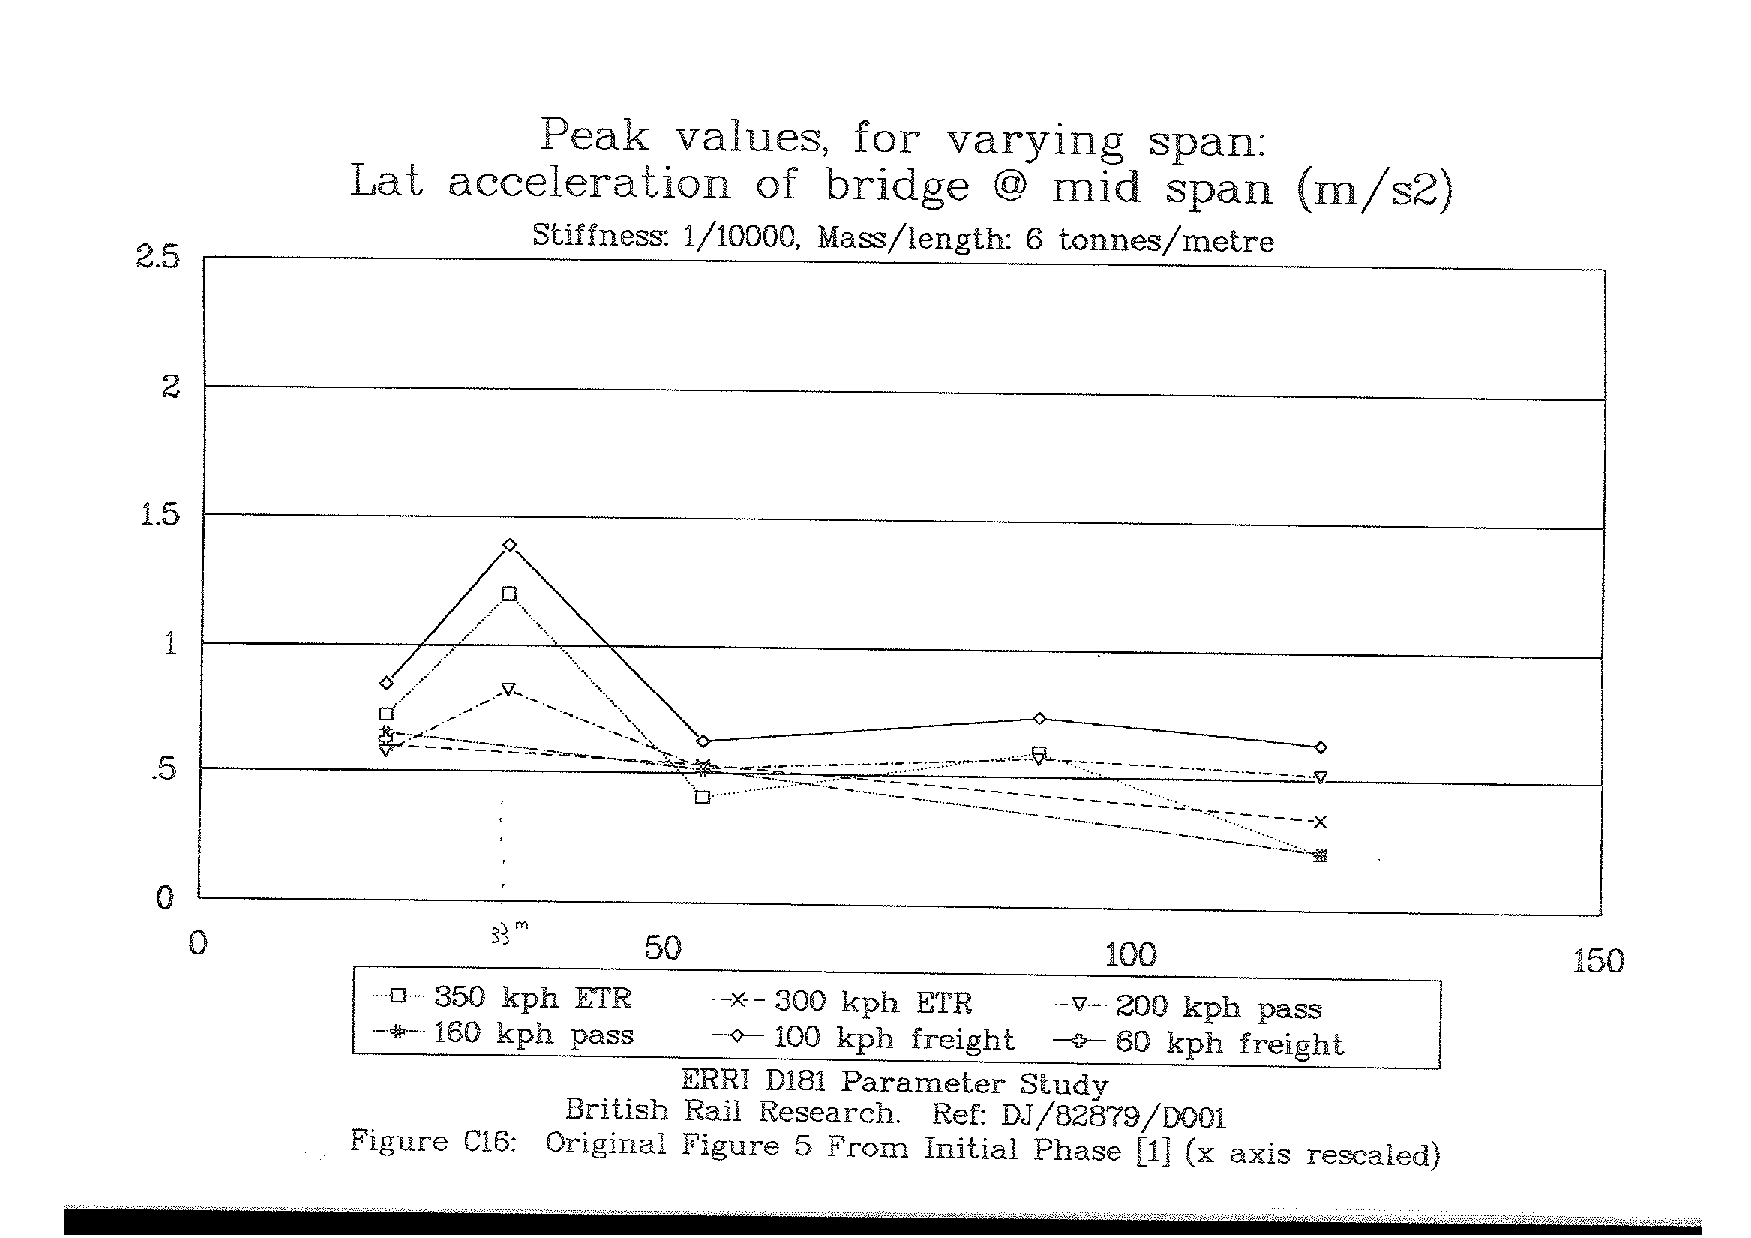
\includegraphics[width=0.8\textwidth]{c16.pdf}
%     \caption{Evidence of resonance caused by kinematic wavelength with span. Extract from \citet[C16]{d181dt329} }
%     \label{fig:c16}
% \end{figure}

% Although wavelength coincidence with span resonance is possible, for longer span bridges (span larger than 50m) it's hardly possible for this type of resonance to build up because the span of the bridge is greater than the wavelength of the train. However, resonance caused by kinematic frequency coincidence with first bending mode is possible even if wavelength and span doesn't match.

% In this report, emphasis is placed on long span bridges, thus resonance cause by kinematic wavelength with span is not investigated due to above reasons. On the other hand, frequencies of kinematic movements of trains will be studied. 

% \section{Conclusion}
% As discussed in Section.\ref{sec:1.2hz} that the origin of natural frequency remains unknown, it is highly doubted that it's actually the frequency range of vehicle suspension system. Rough calculations have been done to study the natural frequencies of the suspension systems of train examples provided in DT 329, proofing all of the frequencies calculated are within a range of 0.3Hz to 1.0Hz. This result mostly overlaps with the frequency range provided by 1.2Hz criterion proposal. 

% If this hypothesis is true, it can also be concluded that D181 committee made a serious mistake in their criterion proposing. Dynamics of the suspension system is only a factor that influence the global dynamic behaviour of a running train, so as track irregularities, train speeds, train layouts, etc. Proposing a criterion based only on natural frequencies of the suspension system is unacceptable. What's more, CEN committee using this proposed criterion in Eurocode 1991-2 was another unconscious mistake.


% \chapter{Train vehicles layouts and geometry}



% \section{Locomotives}
% \subsection{4-axle locomotives}
% Generally, the relevant parameters for categorisation of 4-axle locomotives are axle load P (18 t to 22,5 t) and the bogie axle spacing (2,2 m to 3,4 m).

% Typically the mass per unit length is less than 6,4 t/m and the distance from the end axle to the end of the nearest coupling plane is greater than 1,9 m

% \subsection{6-axle locomotives}

% Generally, the relevant parameters for categorisation of 6-axle locomotives are:

% \begin{enumerate}[-]
% \item the maximum axle load P (18 t to 22 t) in combination with;
% \item the distance between axles within a bogie (1,80 m to 2,25 m).
% \end{enumerate}

% Typically, the mass per unit length (p) is less than 6,4 t/m and the distance from end axle to the end of the nearest coupling plane (a) is greater than 2,1 m.

% \section{Passenger carriages}
 
% \section{Wheelset and track dimensions}

% Generally the track guage is used as a distance measured between the two rails, more specifically the distance between the inside of the railheads measured 14mm below the surface of the rail. By choosing 14 mm the measurement is less influenced by lipping or lateral wear on the rail head and by the radius r = 13 mm of the rail head face. On normal track the gauge is $1435^{+10}_{-3}$ mm with with a maximum gradient of 1:3000. For new track, however, NS apply the following standards:

% \begin{enumerate}
% \item Mean gauge per 200 m: $1435^{+10}_{-1}$ mm
% \item Standard deviation within a 200 m section less than 1 mm
% \end{enumerate}

% \begin{figure}[h]
% \centering
% 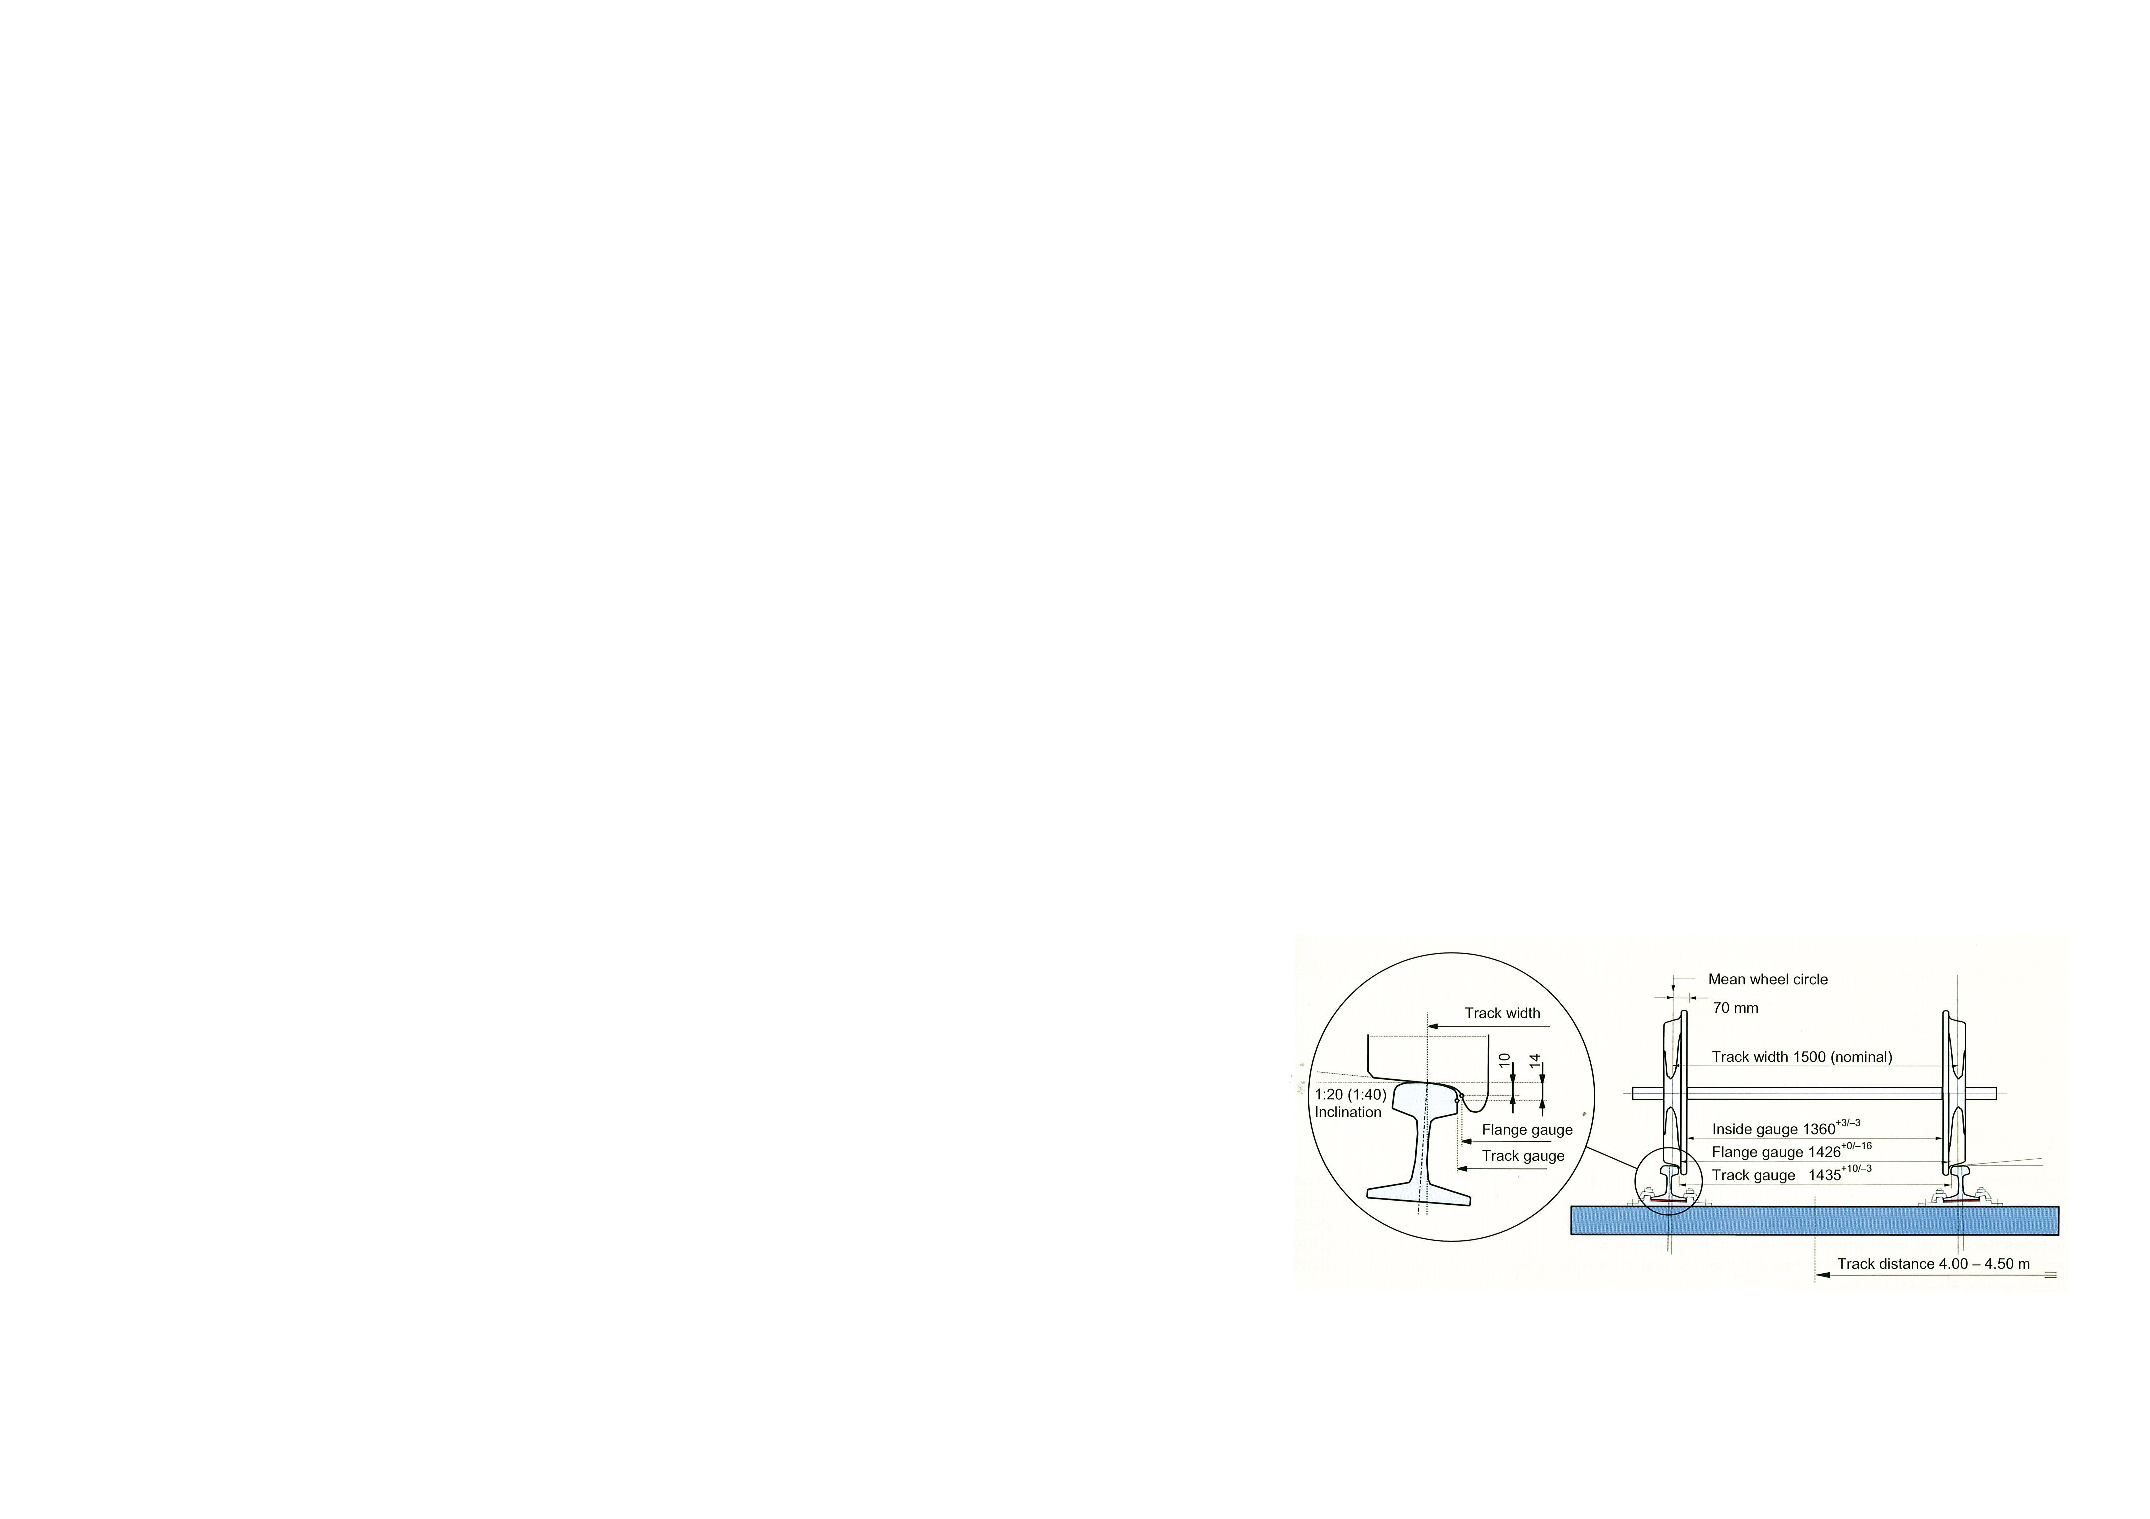
\includegraphics[width=0.8\textwidth]{wheelsettrackdimension.pdf}
% \caption{Wheelset and track dimensions for straight normal gauge track. Extracted from \citet[p.17]{esveld2001modern}}
% \label{fig:wheelset and track dimensions}
% \end{figure}


% \section{Conicity and Equivalent Conicity of Wheels}

% Originally conical tire profiles with an inclination of 1:20 were used. Since a centrally applied load on the railhead is desired, a rail inclination of 1:20, as shown in Figure 2.1, was also selected; this for instance still applies to NS profile NP 46. UIC 54 rail usually has an inclination of 1:40. This inclination matches the S 1002 worn wheel profile which is in general use in Europe. During manufacturing the tires are given a profile which matches the average shape cause by wear. In contrast to the straight conical profile this has a hollow form.

% It is clear that regarding a worn profile the conicity depends on the actual shape of the rail head and tire, including any wear, track gauge, and rail inclination. Likewise, elastic deformation of the wheelset and rail fastenings plays a role.

% Generally, the effective or equivalent conicity is defined as:

% $$ \gamma_e = \frac{\Delta r}{2y} = \frac{r_1 - r_2}{2y}  $$

% Here $r_1 - r_2$ is the instantaneous difference in rolling radius of the wheel treads; generally speaking this is a non-linear function of the lateral displacement y of the wheelset with respect to the central position. The difference between conical and worn profiles is given in Figure.\ref{fig:conicalwornprofiles}. To enable numerical comparisons $\gamma_e$ is determined at a certain lateral displacement $y=\bar{y}$.


% \begin{figure}[h]
%     \centering
%     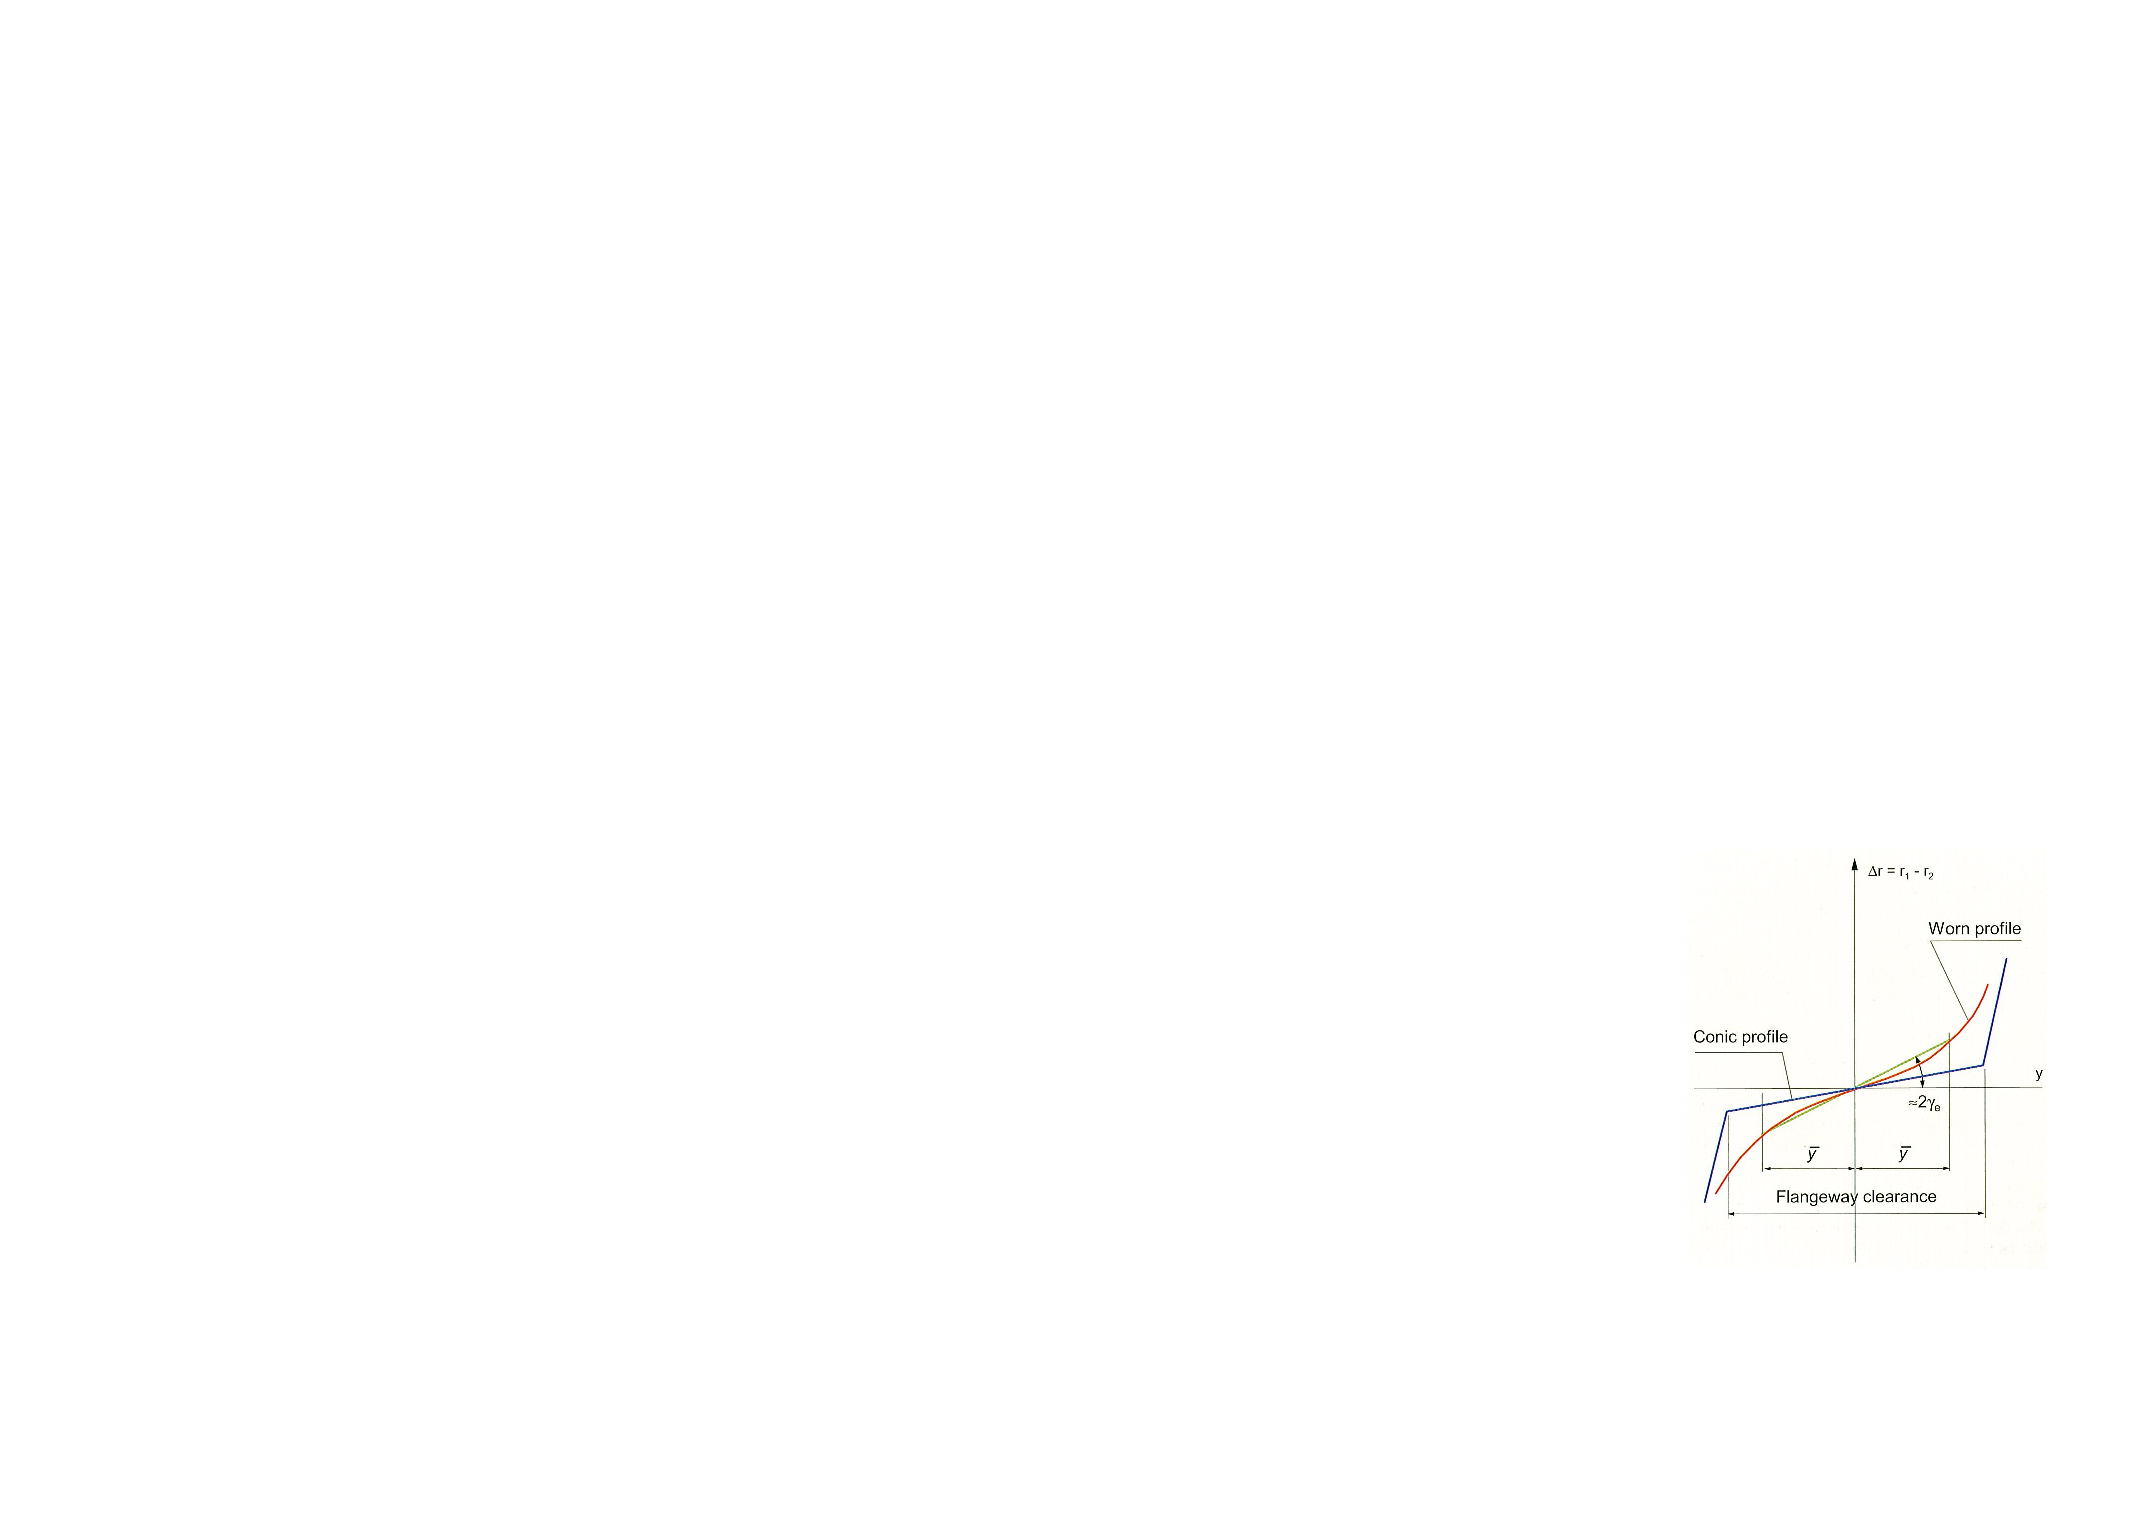
\includegraphics[width=0.6\textwidth]{conicalwornprofiles.pdf}
%     \caption{$y-\Delta r$ curves. Difference between conical and worn wheel profiles. Extracted from \citet[2.4]{esveld2001modern}}
%     \label{fig:conicalwornprofiles}
% \end{figure}

% With a conical profile the conicity is constant and above equation becomes:

% $$ \gamma_e = \frac{\Delta r}{2y} =\frac{(r+\gamma y)-(r-\gamma y)}{2y} = \gamma $$


% \section{Worn wheel profiles}

% A perfectly conical wheel profile is unstable as far as its shape is concerned, but will take on a shape that is stable as the effect of wear.

% Practical research has shown that over a period of time wheel profiles stabilise with wear at an equivalent conicity of 0.2 to 0.3. With regards to running stability, the equivalent conicity must remain below 0.4 and to ensure the centering effect it must be greater than 0.1.

% \section{Trains in Netherlands}

% Passenger trains now in service include following models:

% \begin{enumerate}
%     \item The DD-AR (Dubbeldeksaggloregiomaterieel) \\  EMUs were delivered as DDM-2/3 resembling the bilevel rail cars series DDM-1 from 1985 and operates in fixed formations of 3 or 4 coaches. 4 car trains use a class 1700 locomotive for traction, 3 car trains use an mDDM motorcar, which resembles a DD-AR driving trailer but has electric motors and a single passenger deck on top; the level of this deck is higher than that of a regular single deck rail car, but lower than the upper deck of the other coaches. Three types of coaches are available: Bv (second class), ABv (first and second class) and Bvk (second class driving trailer). The DDM-2/3 series are being modernised from 2010–2013 and after modernisation the series was renamed as NID (Nieuwe Intercity Dubbeldekker).
%     \item The VIRM (Verlengd Interregiomaterieel) \\ also called Regiorunner was partially rebuilt from trainsets DD-IRM (Dubbeldeks Interregiomaterieel). DD-IRM was delivered in 3- and 4-car trainsets. 3-car trainsets got one extra coach, 4-car trainsets got two extra coaches. Also, new 4- and 6-car trainsets were built. Thus, a train consists of one or more combinations of 4 or 6 double deck coaches; each combination (multiple unit) has electric motors. More than three hundred coaches are currently operative in the Netherlands.
%     \item The Koploper (ICM) (Intercitymaterieel) \\ is a 3- or 4-car multiple unit that when coupled with another one, allows passengers to walk through (the name Koploper being a play on words – literally "head walker", but in actual use meaning "front runner"). The Dutch Railway Company decided to close the heads permanently on 31 October 2005 because the mechanism broke down too often. A scheduled modernisation of around 7 million euro will see the ICM fleet updated. The renovated ICM trains provide 13\% more seats (reducing the leg room to uncomfortable small for the long haul journeys they serve in 2nd class, which is further aggravated by a waste bin that is placed on the backsides of the seats in front), have a new interior, a bathroom accessible by wheelchairs, airconditioning as well as upgrades to the engine and connection systems. The head doors are removed. Also, these (renovated) trains are the first trains in the NS fleet equipped with OBIS. OBIS provides a (free) WiFi-connection on board, along with in-train journey information provided through screens and (automated) vocal announcements through the trains speakers. This journey information provides the actual status, and thus is always up-to-date to the actual situation this trip, and the stations is passes.
%     \item The Sprinter (SGM, Stads Gewestelijk Materieel) \\ is a two or three car electric, used on small distances. They are named Sprinter because they're able to accelerate and brake quite fast, making them very suitable for 'stoptrein' services. They were also specifically designed for urban environments where they run commuter services. As a result, they are most commonly found in the Randstad area. The initial idea was that the Sprinter would provide somewhat of a subway/metro service but this plan failed as the cities of Amsterdam and Rotterdam continued to construct their own rapid transit systems. Nevertheless, in the densely populated Randstad, the Sprinters remain popular. Two car versions were revised and renamed to Citypendel. All Sprinters are now refurbished into the new white/yellow/dark blue livery.
% \end{enumerate}

% All of passenger train coaches have a wheel diameter of 920 mm. 

% Locomotives of freight trains have wheel diameter of 1000 mm.

% \section{Lateral Track Irregularities}
% This section describes allowable lateral track irregularities defined in EN13848-5\citet{13848}. 

% Lateral alignment irregularities was defined in EN13838-1. It states:"Deviation $y_p$ in y-direction of consecutive positions of point P... on any rail, expressed as an excursion from the mean horizontal position (reference line) covering the wavelength ranges stipulated below and calculated from successive measurements ...". See Figure \ref{fig:lateraldeviationdefine}.

% For lateral deviations, the following wavelengths shall be considered: $D1 = 3 -25 m$, $D2 = 25 - 70 m$ and $D3 = 70 - 200 m$. 

% \begin{figure}[h]
%     \centering
%     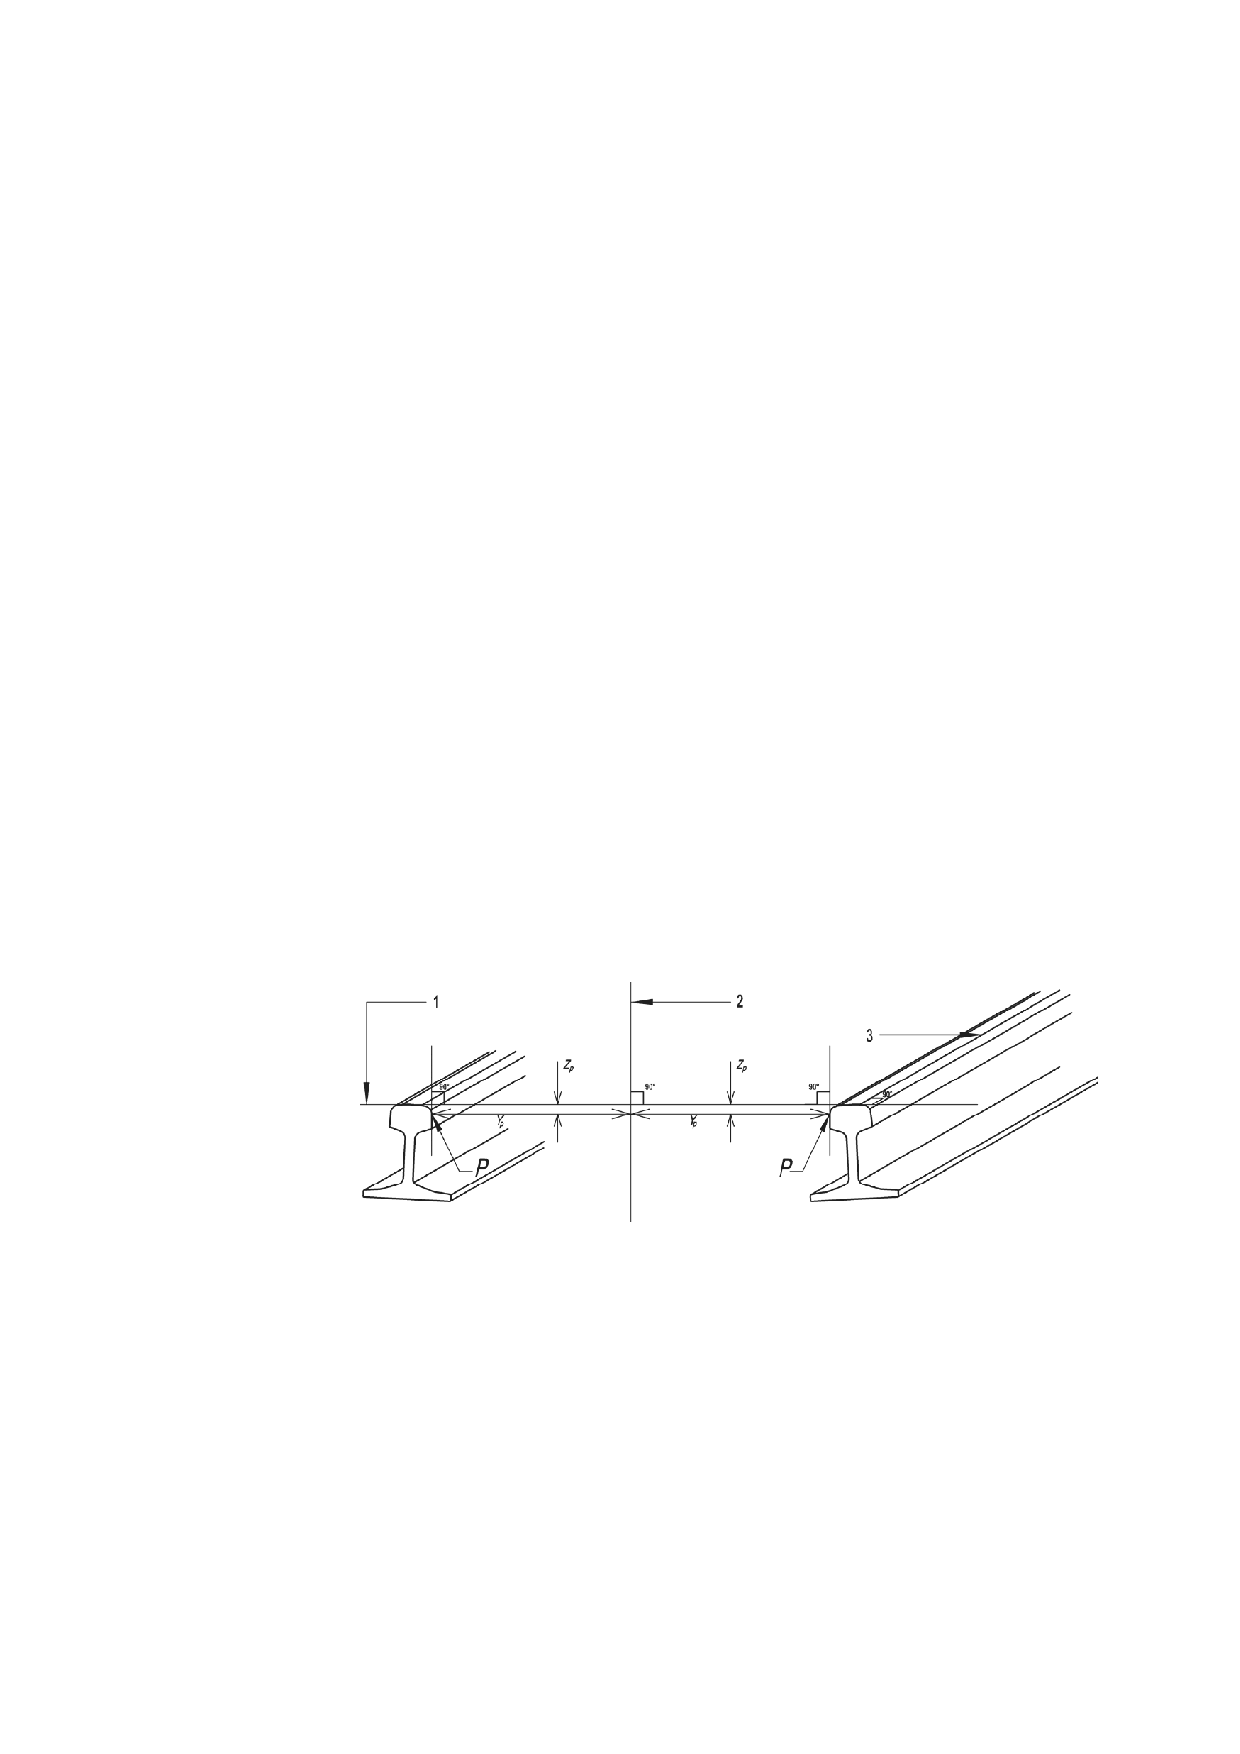
\includegraphics[width=0.8\textwidth]{lateraldeviationdefine}
%     \caption{Lateral deviation definition. Lateral deviations $y_p$ for each rail with 1: running surface, 2: reference line and 3: centre line of running table}
%     \label{fig:lateraldeviationdefine}
% \end{figure}

% Table \ref{tab:lateraldeviation} defines the allowable standard deviation for lateral track irregularities.

% \begin{table}[h]
%     \centering
%     \caption{Alignment - AL - Standard deviation. Extracted from \citet[Table B.6]{13848}}
%     \begin{tabular}{cc}
%         \hline
%         Speed(km/h) & Standard deviation(mm) \\
%         \hline
%         $V\leq 90$ & 1.5 to 1.8 \\
%         $80 < V \leq 120$ & 1.2 to 1.5 \\
%         $120 < V \leq 160$ & 1.0 to 1.3 \\
%         $160 <V \leq 230$ & 0.8 to 1.1 \\
%         $230 <V \leq 300$ & 0.7 to 1.0 \\
%         \hline
%     \end{tabular}
%     \label{tab:lateraldeviation}
% \end{table}


\chapter{Lateral wavelength research on Dutch railway vehicles}\label{sec:wavelengthstudy}

As a conclusion in DT329 report, the lateral dynamic effects of railway vehicles are all wavelength phenomenon. The lateral wavelength of trains is a constant characteristics of themselves which doesn't change with outer environment. However, while the wavelength for axle repeat pattern is easy to get, the wavelength for kinematic movement normally requires heavy FEM simulations and post analysis of the response spectrum. 

Although it has been concluded in the previous chapter that avoiding resonance frequency is not a correct strategy for dynamics design in general, investigating the wavelength of trains can serve for the practical analysing methods that will be developed in following chapters in an alternative way.

This research aims to investigate both wavelength of trains running in the Netherlands. The axle repeat pattern wavelength is created by collecting all the possible axle layouts. The kinematic movement wavelength is created by developing a approximate methods that avoids heavy FEM simulations. 


\section{Effects investigated in wavelength study}

Effects investigated in this report will be the same effects investigated in DT 329, which is described in Sec.\ref{sec:resonance329}. However, according to the statement in Sec.2.3[Summary of results] in the same report,

\begin{quote}
Even when the axle repeat frequency matches the first lateral bending mode of each span, there is no evidence that the resonant behaviour of the span and train has any effect on subsequent spans, since the resonant effects do not appear to grow from span to span.
\end{quote}

the third investigated resonance effect 'coincidence between the length of the span and the kinematic wavelength of the trailing vehicles' is neglected in this thesis because it is concluded in \citet{d181dt329} that resonance do not grow from span to span. 


\section{Equivalent conicity used in this study}
According to \citet[Section.2.6]{esveld2001modern}, 

\begin{quote}
    Practical research has shown that over a period of time wheel profiles stabilise with wear at an equivalent conicity of 0.2 to 0.3. With regards to running stability, the equivalent conicity must remain below 0.4 and to ensure the centering effect it must be greater than 0.1.
\end{quote}

conicity range will be 0.2 to 0.3.

It is suggested by this report that vehicle maintenance sector ensure wheels of train wheels stay in the safe zone of conicity. 


\section{Study on wavelength of lateral kinematic movement}

The kinematic movememnt of the train on the rail is much similar to klingel movement. This section aims to assess the capability of using klingel formula to predict the wavelength of the whole train.

Klingel movement is proposed by Klingel which can well predict the moving trend of a single wheelset on a straight railway track. However, the kinematic movement of a certain wheelset assembled into a running train is different from the movement of a single free wheelset. This is due to multiple bodies interact with each other, introducing more complicated mechanism in wheel/rail interaction. 

This  study focuses on Klingel movement of a bogie. First part of the  study will try to discuss the relationship of Klingle frequency of a wheelset and kinematic movement frequency of a whole train. Second part of the study will use realistic data of Dutch railway/vehilces to assess the frequency bandwidth of Dutch native trains.

This section will include following parameters to be studied:

\begin{enumerate}[-]
	\item Speed of train, radius of the wheel and conicity of the wheel. 
	\item Gauge distance is fixed to 1435mm according to UIC standard. 
	\item Frequency is linear to speed if other parameters are fixed.
\end{enumerate}


\subsection{Comparison between Klingle movement and train kinematic movement studied in D181 DT329}

In this section the kinematic wave length of trains used in D181 VAMPIRE simulations will be calculated by klingel's formula and compared with the wavelength value obtained in VAPIRE simulation.

Klingel's formula:
Klingel has done experiments and has given that the wavelength of a single wheelset:

$$ \lambda_0 = 2 \pi \sqrt{\frac{rG}{2\gamma} }$$

where:

G = Dynamic Gauge

r = Dynamic Wheels Radius

g = Conicity

For 2 wheelsets connected by a bogie:

$$ \lambda = \lambda_0 \sqrt{1+(\frac{I}{G})^2}  $$

where:

I = Rigid wheel base

By inputting the related train parameters used in VAMPIRE simulations into the Klingel formula, following table is obtained.

\begin{table}[h]
  \centering
  \caption{Approxiamte letaral kinematic wavelength calcualted by improved Klingel formula}
    \begin{tabular}{cccccccccccccccc}
    \toprule
    & Gauge & BWD & Radius & Conicity & Wavelength($\lambda_0$) &Wavelength($\lambda$) & \\
    \midrule
    BR CLASS 56 LOCO  & 1435 & 4180 & 290 & 0.05 & 12.8175 & 39.4750 \\
    FS E444 LOCO  & 1435 & 2600 & 550 & 0.05 & 17.6517 & 36.5301 \\
    FS ETR500 LOCO  & 1435 & 3000 & 550 & 0.05 & 17.6517 & 40.9070\\
    UIC FREIGHT WAGON  & 1435 & 0 & 460 & 0.05 & 16.1430 & 16.1430 \\
    FS ETR500 COACH  & 1435 & 3000 & 440 & 0.05 & 15.7882 & 36.5883 & \\
    UIC COACH  & 1435 & 2560 & 445 & 0.05 & 15.8776 & 32.4718 &  \\
    \bottomrule
    \end{tabular}%
  \label{tab:wavelengthkinematic}%
\end{table}%


By comparing the result from Table.\ref{tab:wavelengthkinematic} and kinematic wavelength obtained by D181, extracted as Table.\ref{tab:329kinematicwavelength}, parametric study results show close prediction for kinematic wavelength of freight train locomotive/coach/wagon. It's because freight train suspension system is simpler and stiffer compared to passenger train's, making the behaviour of train acts more similar to the behaviour of a single wheelset of bigger mass. 


Wavelength for UIC freight wagon is a special case and it's not meeting the wavelength results in VAMPIRE simulations. This is probably because this car has a different design. It can be seen from in Figure.\ref{fig:uicoach} that only 2 axles are installed and there's no wagon installed. See Figure.\ref{fig:2axlefreight} and Figure.\ref{fig:4axlefreight} for their different axle configurations.

\begin{figure}[h]
	\centering
	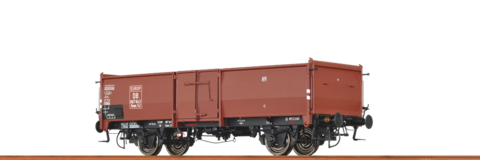
\includegraphics[width=0.5\textwidth]{2alxefreight.png}
	\caption{Example of a 2-axle freight wagon}
	\label{fig:2axlefreight}
\end{figure}

\begin{figure}[h]
	\centering
	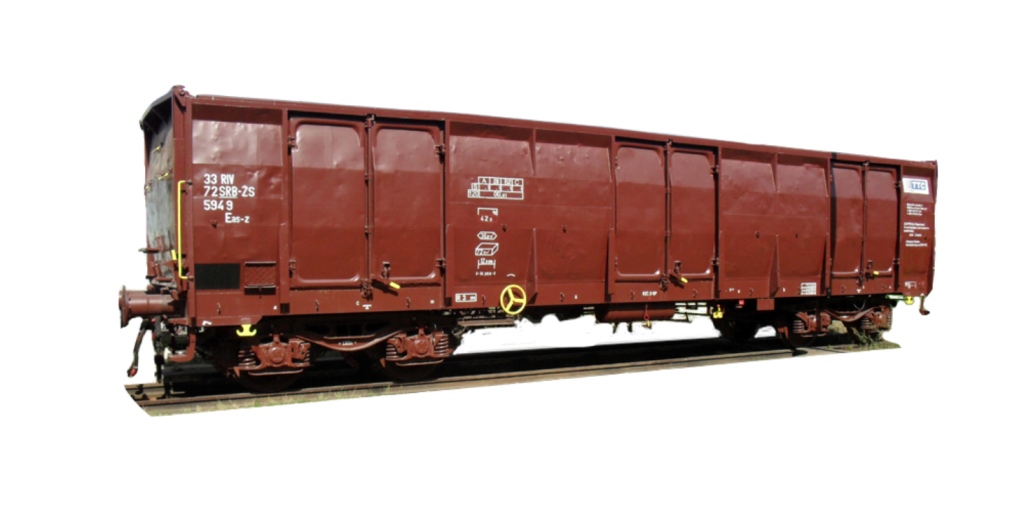
\includegraphics[width=0.5\textwidth]{4alxefreight.png}
	\caption{Example of a 4-axle freight wagon}
	\label{fig:4axlefreight}
\end{figure}


The train parameter used in this part of parametric study is attached in the Appendix.\ref{app:mu}. 


\section{Assess of wavelength bandwidth based on realistic data of Dutch Rail/Vehicle}

The wavelength of passenger coach is highly related to the characteristics of its suspension systems. These data are often difficult to obtain. Since the improved Klingel formula ignored the effect of suspension system, the results in this section is only approximate value for the wavelength of kinematic movement.


Future research is highly recommended to be conducted to study the kinematic wavelength of complete vehicles in the Netherlands, using realistic data of their suspension systems.


Table.\ref{tab:wavelengthrealistic} is created by processing Dutch wheel radius and wheelbase data collected from document\citet{trainparameters}. 
Thus range of $\lambda$ is obtained by inputting realistic data in Kingel formula, illustrated in Table.\ref{tab:wavelengthrealistic}.

\begin{table}[h]
  \centering
  \caption{Wavelength of kinematic movement generated by realistic value}
    \begin{tabular}{cccccccccccccccc}
    \toprule
    & Gauge & BWD & Radius & Conicity & Wavelength\_0() &Wavelength & \\
    \midrule
    \textbf{Freight 2-axle} & 1435 & 0 & 500 & 0.05 & 16.8303 & 16.8303 \\
    \textbf{} & 1435 & 0 & 500 & 0.2 & 8.4151 & 8.4151  \\
    \textbf{} & 1435 & 0 & 500 & 0.3 & 6.8709 & 6.8709  \\
    \textbf{}       &       &       &       &       &       &       &  \\
    \textbf{Freight 4-axle} & 1435 & 1800 & 500 & 0.05 & 16.8303 & 26.9988 \\
    \textbf{} & 1435 & 1800 & 500 & 0.2 & 8.4151 & 13.4994  \\
    \textbf{} & 1435 & 1800 & 500 & 0.3 & 6.8709 & 11.0222  \\
    \textbf{}       &       &       &       &       &       &       &  \\
    \textbf{Passenger} & 1435 & 2500 & 460 & 0.05 & 16.1430 & 32.4275 \\
    \textbf{} & 1435 & 2500 & 460 & 0.2 & 8.0715 & 16.2137  \\
    \textbf{} & 1435 & 2500 & 460 & 0.3 & 6.5904 & 13.2385 \\
    \textbf{}       &       &       &       &       &       &       &  \\
    \textbf{} & 1435 & 2750 & 460 & 0.05 & 16.1430 & 34.8947 \\
    \textbf{} & 1435 & 2750 & 460 & 0.2 & 8.0715 & 17.4473  \\
    \textbf{} & 1435 & 2750 & 460 & 0.3 & 6.5904 & 14.2457  \\
    \textbf{}       &       &       &       &       &       &       &  \\
    \textbf{Locomotive} & 1435 & 2400 & 500 & 0.05 & 16.8303 & 32.7960 \\
    \textbf{} & 1435 & 2400 & 500 & 0.2 & 8.4151 & 16.3980  \\
    \textbf{} & 1435 & 2400 & 500 & 0.3 & 6.8709 & 13.3889  \\
    \textbf{}       &       &       &       &       &       &       &  \\
    \textbf{} & 1435 & 2950 & 500 & 0.05 & 16.8303 & 38.4751 \\
    \textbf{} & 1435 & 2950 & 500 & 0.2 & 8.4151 & 19.2376  \\
    \textbf{} & 1435 & 2950 & 500 & 0.3 & 6.8709 & 15.7074  \\
    \bottomrule
    \end{tabular}%
  \label{tab:wavelengthrealistic}%
\end{table}%

For conservative usage, please take the value yielded by 0.3 wheel conicity. However, as proved in previous section, this estimation is in closest estimation of simulation results when concity is 0.05.

% Figure.\ref{fig:wavelengthkinematicfreight} and Figure.\ref{fig:wavelengthkinematicpass} are generated according to linear relationship between frequency and speed, using the wavelength $\lambda$ obtained in Table.\ref{tab:wavelengthrealistic}:

% $$ f = v \frac{1}{\lambda} $$


% \begin{figure}[h!]
% \centering
% \begin{tikzpicture}[trim axis left, trim axis right]
% \begin{axis}[
%     xlabel={$v(m/s)$},
%     ylabel={$f(Hz)$},
%     ymin = 0, xmin = 0, xmax = 44.4,
%     legend entries={$\sfrac{1}{\lambda}=0.059$,$\sfrac{1}{\lambda} =0.072$,$v=33.3 m/s$,$f=0.3Hz$},
%     grid = both,
%     minor y tick num= 4,
%     minor x tick num= 4,
%     legend pos = north west,
% ]
% \addplot[blue, domain = 0:44.4,samples=201,name path = A]{0.059*x};
% \addplot[red, domain = 0:44.4,samples=201, name path = B]{0.072*x};
% \addplot[mark=none, dashed]  coordinates {(33.3,0) (33.3,5) };
% \addplot[domain = 0:44.4,samples=10,dashed]{0.3};
% \addplot[gray] fill between[of=A and B];
% \end{axis}
% \end{tikzpicture}
% \caption{Lateral frequency of freight train with respect to speed(Kinematic movement)}
% \label{fig:wavelengthkinematicfreight}
% \end{figure}

% \begin{figure}[h!]
% \centering
% \begin{tikzpicture}[trim axis left, trim axis right]
% \begin{axis}[
%     xlabel={$v(m/s)$},
%     ylabel={$f(Hz)$},
%     ymin = 0, xmin = 0, xmax = 44.4,
%     legend entries={$\sfrac{1}{\lambda}=0.062$,$\sfrac{1}{\lambda}=0.076$,$v=33.3 m/s$,$f=0.3Hz$},
%     grid = both,
%     minor y tick num= 4,
%     minor x tick num= 4,
%     legend pos = north west,
% ]
% \addplot[blue, domain = 0:44.4,samples=201, name path = A]{0.062*x};
% \addplot[red, domain = 0:44.4,samples=201, name path = B]{0.076*x};
% \addplot[mark=none,dashed]  coordinates {(33.3,0) (33.3,3.5) };
% \addplot[domain = 0:44.4,samples=10,dashed]{0.3};
% \addplot[gray] fill between[of=A and B];
% \end{axis}
% \end{tikzpicture}
% \caption{Lateral frequency of passenger train with respect to speed(Kinematic movement)}
% \label{fig:wavelengthkinematicpass}
% \end{figure}

\section{Lateral wavelength of axle repeat pattern of Dutch Railway Vehicles}

This section will generate lateral wavelength value of axle repeat pattern of Dutch Railway Vehicles. Although DT329 provided wavelength values for some trains in Table.\ref{tab:329axlerepeat} but the way of obtaining these values was not mentioned. So an interpretation is needed to understand how to obtain the axle repeat pattern wavelength.

By observing Table.\ref{tab:329axlerepeat}, it can be seen that axle spacing layout is the only raw data needed to generate axle repeat pattern wavelength. The value is regardless of all other parameters. There are several axle space combinations in the table, but only one combination was finally put emphasis on during the analysis phase of axle repeat resonance research. They are

\begin{enumerate}[-]
    \item \textit{'wagon n axle m - wagon n+1 axle m'} for freight train, 
    \item \textit{'coach n axle m - coach n+1 axle m'} for passenger train,
    \item \textit{'coach n axle m - coach n+1 axle m'} for high speed train.
\end{enumerate}

It's still hard to comprehend above combinations so further interpretation is done by comparing it to train parameters in Appendix.\ref{app:dt329data}. It is found 

By comparing Fig.\ref{fig:trainparameters} and Table.\ref{tab:329axlerepeat}. It can be seen that 'wagon n axle m - wagon n+1 axle m' means the distance between one axle in the previous car and another axle in next car in the same location. The same goes for passenger train and high speed train. To better understand this spacing, please see L\_Coa in Figure.\ref{fig:trainparameters}. 

\begin{table}[h!]
  \centering
  \caption{Wavelength of axle repeat pattern($m$)}
    \begin{tabular}{rrrrrrrrr}
    \toprule
    \textbf{Type} & \textbf{L\_coa min} & \textbf{L\_coa max} & \textbf{2*L\_coa min } & \textbf{2*L\_coa max} \\
    \midrule
    \textbf{CB\_1} & 23.8  & 25.3  & 47.6  & 50.6 \\
    \textbf{CB\_2} & 25.3  & 27.5  & 50.6  & 55    \\
    \textbf{AB\_1} & 14.9  & 16    & 29.8  & 32     \\
    \textbf{AB\_2} & 18.8  & 19.5  & 37.6  & 39    \\
    \textbf{AB\_3} & 17    & 17.5  & 34    & 35   \\
    \textbf{AB\_4} & 18.7  & 19.2  & 37.4  & 38.4  \\
    \textbf{SA\_1} & 9.2   & 9.8   & 18.4  & 19.6  \\
    \textbf{SA\_2} & 12.8  & 13.5  & 25.6  & 27    \\

    \bottomrule
    \end{tabular}%
  \label{tab:wavelengthaxlerepeat}%
\end{table}%

Lateral wavelength of axle repeat pattern is then obtained by extracting all possible L\_Coa values from MU standards in \citet{EC15528}, illustrated in Table.\ref{tab:wavelengthaxlerepeat}. Detailed information about MU classes can be found in Appendix.\ref{app:mu}.


After examing the content in analysing section of DT329 resonance study, it is found that double length of L\_Coa is not taken into account in analysis phase. This means although D181 committee calculated double length of L\_Coa, these values were never used. Thus it is advisable for the usage of lateral axle repeat pattern wavelength, extracting only L\_Coa min column and L\_Coa max column.


% \begin{figure}[h!]
% \centering
% \begin{tikzpicture} 
%     \begin{axis}[
%     xlabel={$v(m/s)$},
%     ylabel={$f(Hz)$},
%     ymin = 0, xmin = 0, xmax = 44.4,
%     %legend entries={$i=0.057$,$i=0.07$,$v=33.3 m/s$,$f=0.3Hz$},
%     grid = both,
%     minor y tick num= 4,
%     minor x tick num= 4,
%     ]
%     \addplot[blue,name path=A,domain=0:44.4] {0.036*x};
%     \addplot[red, name path=B,domain=0:44.4] {0.042*x};
%     \addplot[black] fill between[of=A and B];
%     \addplot[blue,name path=C,domain=0:44.4] {0.051*x};
%     \addplot[red, name path=D,domain=0:44.4] {0.053*x};
%     \addplot[black] fill between[of=C and D];
%     \addplot[blue,name path=E,domain=0:44.4] {0.057*x};
%     \addplot[red, name path=F,domain=0:44.4] {0.059*x};
%     \addplot[black] fill between[of=E and F];
%     \addplot[blue,name path=G,domain=0:44.4] {0.063*x};
%     \addplot[red, name path=H,domain=0:44.4] {0.067*x};
%     \addplot[black] fill between[of=G and H];
%     \addplot[blue,name path=I,domain=0:44.4] {0.074*x};
%     \addplot[red, name path=J,domain=0:44.4] {0.078*x};
%     \addplot[black] fill between[of=I and J];
%     \addplot[blue,name path=K,domain=0:44.4] {0.102*x};
%     \addplot[red, name path=L,domain=0:44.4] {0.109*x};
%     \addplot[black] fill between[of=K and L];
%     \addplot[blue,name path=M,domain=0:44.4] {0.018*x};
%     \addplot[red, name path=N,domain=0:44.4] {0.021*x};
%     \addplot[gray] fill between[of=M and N];
%     \addplot[blue,name path=O,domain=0:44.4] {0.026*x};
%     \addplot[red, name path=P,domain=0:44.4] {0.027*x};
%     \addplot[gray] fill between[of=O and P];
%     \addplot[blue,name path=Q,domain=0:44.4] {0.029*x};
%     \addplot[red, name path=R,domain=0:44.4] {0.029*x};
%     \addplot[gray] fill between[of=Q and R];
%     \addplot[blue,name path=S,domain=0:44.4] {0.031*x};
%     \addplot[red, name path=T,domain=0:44.4] {0.034*x};
%     \addplot[gray] fill between[of=S and T];
%     \addplot[blue,name path=U,domain=0:44.4] {0.037*x};
%     \addplot[red, name path=V,domain=0:44.4] {0.039*x};
%     \addplot[gray] fill between[of=U and V];
%     \addplot[blue,name path=W,domain=0:44.4] {0.051*x};
%     \addplot[red, name path=X,domain=0:44.4] {0.054*x};
%     \addplot[gray] fill between[of=W and X];
%     \addplot[dashed,thick,red, domain=0:44.4] {0.3};
% \end{axis}
% \end{tikzpicture}
% \caption{Two repeat pattern frequencies with respect to speed}
% \label{fig:repeatpatternfrequencies}
% \end{figure}

\section{Conclusion of wavelength study}

The lateral resonance effects between running train and railway bridge include two phenomenon: Axle repeat pattern and Kinematic movement. Those two phenomenon are all wavelength phenomenon, which means for every specific train, the wavelength of its axle repeat pattern and kinematic movement remains constant. In other word, the frequency of lateral dynamic effect caused by the operating of trains on bridge is directly related to the speed.

Since the wavelength for the two phenomenon on the same train are not likely to be equal, the possible range of wavelength for both phenomenon were investigated in this chapter. The possible axle repeat pattern wavelength is approximately 10m-30m covering all train types and kinematic wavelength is 13m to 17m covering all train types. It can be seen that axle repeat pattern possess a broader range of wavelength than kinematic movement.

It also can be concluded that for any railway bridge, resonance between the bridge itself and train can happen if the train is running at a corresponding resonance speed according to its wavelength. So avoiding resonance is not a valid strategy to choose, not to mention the apparent frequency shift phenomenon to be discussed in Chapter.\ref{sec:resonance329}. 

To be noted that these wavelength are also not the exact wavelength in real-life scenario but an estimation, especially for kinematic movement. But it gave away a rough idea about the magnitude of trains' wavelength, and, can be used for practical design purposes. To see the usage of studied wavelength, please see Chapter.\ref{sec:parcticalmethod}



\chapter{Essentials of analytical approach to be adopted in practical checking method}\label{sec:analyticalmodel}
 
\section{Introduction}
This chapter aims to give a preliminary knowledge of a selected analytical model that simulates the perfect resonance scenario for railway bridge under lateral dynamic load. The knowledge contains the simplified model itself, its assumptions, field of application and explicit solutions. 

The output response of the solution to the analytical model is able to provide the maximum bridge response in worst case scenario. Thus it is sufficient to be adopted in practical purposes for verifications of lateral railway bridge dynamics.


\section{Overview}

To give a clear view of this chapter, following overview is created:

\begin{enumerate}
    \item The model, its assumptions and field of application. 
    \item Procedure of solution deduction
    \item Damping
\end{enumerate}

\section{The model, its assumptions and field of application}

\begin{figure}[h]
    \centering
    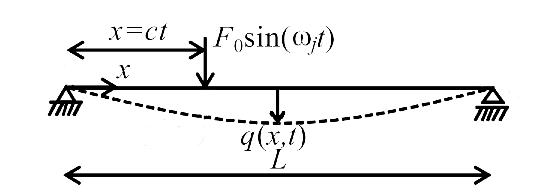
\includegraphics[width=0.5\textwidth]{harmonicloadbeam}
    \caption{Schematic representation of a generic beam crossed by a harmonic load}
    \label{fig:harmonicloadbeam}
\end{figure}

Presented in Figure.\ref{fig:harmonicloadbeam}, the model features a simply supported beam which is the simplification of bridge structure and a moving harmonic load introducing resonant dynamic effects caused by the presence of moving train.

The beam is assumed to be uniform in both geometry and material. The stiffness of the beam is the equivalent uniform lateral bending stiffness of the bridge. 

The load is moving in the same speed as the train. The magnitude of load amplitude is going to be discussed in the following chapter. The load's self vibration frequency is equal to the first natural lateral bending frequency of the beam.


This model is valid for single span railway bridges that has a sinuous first natural lateral vibration shape.  

\section{Solution deduction}

Solution provided by Fryba\citet{fryba1999vibration} is used to analyse the problem. A harmonic moving along a beam is a fundamental dynamics topic and was first solved by S.P.Timoshenko. Fryba further deduced the basic results, and set them forth in the form of useful formulae. This model is used to simulate a perfect resonance scenario which yields conservative results for designing and checking of the dynamics behaviour of the bridge. Deduction procedure is extracted from \citet[Section II.2.1]{fryba1999vibration} and presented below.

\begin{quote}

The solution of the problem of a harmonic concentrated force moving at constant speed $c$ over a simply supported beam with span $l$ is carried out under the same assumptions as that discussed in Chap. 1. The time-variable concentrated force is of the form

\begin{equation}
    P(t) = Q \sin \Omega t
\end{equation}

where $Q$ is the amplitude and $\Omega$ is the circular frequency of the harmonic force. Vibration of the beam is then described by the equation

\begin{equation}\label{eq:equationofmotion}
    EJ\frac{\partial^4 v(x,t)}{\partial x^4} + \mu\frac{\partial^2 v(x,t)}{\partial t^2} +2\mu\omega_b \frac{\partial v(x,t)}{\partial t} = \delta(x-ct)Q\sin\Omega t 
\end{equation}

by the boundary conditions (1.2) and by the initial conditions (1.3). The symbols used in \ref{eq:equationofmotion} have the same meaning as those of Chap. 1.

Eq.\ref{eq:equationofmotion} together with conditions (1.2) and (1.3) will again be solved by the method of integral transformations. Following the Fourier sine transformation according to (1.9), Eqs.\ref{eq:equationofmotion} and (1.2) give

\begin{equation}
    \frac{d^2 V(j,t)}{d t^2} + 2\omega_b\frac{dV(j,t)}{dt} + \omega_{(j)}^2 V(j,t) = \frac{Q}{\mu} \sin\Omega t \sin j\omega t
\end{equation}

Solving the above with (1.3) by the Laplace-Carson transformation (1.15) - making use of Eq.(27.24) in doing so and of the notation

\begin{equation}
    \begin{tabular}{cc}
        $r_1 = \Omega + j\omega$; & $r_2 = \Omega - j\omega$ \\
    \end{tabular}
\end{equation}

we get

\begin{equation}\label{eq:V*}
    V^* (j,p) = \frac{Q}{2\mu} (\frac{1}{p^2+r_2^2}-\frac{1}{p^2+r_1^2})\frac{p^2}{(p+\omega_b)^2+\omega_{(j)}^{'2}}
\end{equation}

After inverse transformations of Eq.\ref{eq:V*} according to (27.24) and (1.9) the required result for $t \leq T$ is

\begin{dmath}\label{eq:v(x,t)complicated}
    v(x,t) = \sum_{j=1}^{\infty} \frac{Q}{\mu l}\{\frac{1}{(\omega_{(j)}^2 - r_2^2)+4\omega_b^2r_2^2}[(\omega_{j}^2-r_2^2])(\cos r_2t-e^{-\omega_bt}\cos \omega_{(j)}^' t) + 2\omega_b r_2 \sin r_2 t - \frac{\omega_b}{\omega_{(j)}^'}(\omega_{(j)}^2 + r_2^2)e^{-\omega_b t}\sin \omega_{(j)}^'t]-\frac{1}{(\omega_{(J)}^2 - r_1^2)^2 + 4\omega_b^2r_1^2}[(\omega_{(j)}^2-r_1^2)(\cos r_1t-e^{-\omega_b t}\cos\omega{(j)}^'t)+2\omega_b r_1 \sin r_1 t- \frac{\omega_b}{\omega_{(j)}^'}(\omega_{(j)}^2+r_1^2)e^{-\omega_b t}\sin \omega_{(j)}^' t]\}\sin\frac{j\pi x}{l}
\end{dmath}

We shall now simplify Eq.\ref{eq:v(x,t)complicated} to fit the case most frequently met with in practical applications. Thus, for example, it is entirely satisfactory to use only the first of its terms($j=1$); further, as we know from Chap. 1, parameters $\alpha$ and $\beta$ are usually much smaller than 1 ($\alpha = \sfrac{\omega}{\omega_{(1)}} \ll 1$, $\beta = \sfrac{\omega_b}{\omega_{(1)}} \ll 1$). And finally, since in practice a harmonic force is always accompanied by a constant force $P$, we shall introduce in \ref{eq:v(x,t)complicated} also the deflection $v_0$ according to (1.21). Following these simplifications Eq.(2.6) takes on the form

\begin{dmath}\label{eq:v(x,t)withP}
v(x,t) = v_0 \frac{Q}{p}\frac{\omega_{(1)}^2}{\Omega^2}\frac{1}{(\frac{\omega_{(1)}^2}{\Omega^2}-1)^2+4(\frac{\omega^2}{\Omega^2}+\frac{\omega_b^2}{\Omega^2})}\{[(\frac{\omega_{(1)}^2}{\Omega^2}-1)^2+4\frac{\omega_b^2}{\Omega^2}]^{\sfrac{1}{2}} \sin (\Omega t + \varphi)\sin \omega t + 2\frac{\omega}{\Omega}(\cos \Omega t \cos \omega t - e^{-\omega_b t}\cos \omega_{(1)}t)\}\sin\frac{\pi x}{l}
\end{dmath}

where

\begin{equation}
    \tan \varphi = -\frac{2\sfrac{\omega_b}{\Omega}}{\sfrac{\omega_{(1)}^2}{\Omega^2}-1}
\end{equation}

The beam reaches the state of highest dynamic stressing in the region of resonance, i.e. whenever $\Omega$ is close or just equal to $\omega_{(1)}$, i.e.

\begin{equation}
    \Omega = \omega_{(1)}
\end{equation}

In such a case Eq.\ref{eq:v(x,t)withP} can further be simplified to 

\begin{equation}\label{eq:v(x,t)simplewithP}
    v(x,t) = v_0 \frac{Q\omega_{(1)}}{2P}\frac{\cos \omega_{(1)}t}{\omega^2+\omega_b^2}[\omega(\cos\omega t - e^{-\omega_b t})-\omega_b\sin\omega t]\sin\frac{\pi x}{l}
\end{equation}

\end{quote}

According to (1.21)

\begin{equation}
    v_0 = \frac{Pl^3}{48EJ} \approx \frac{2P}{\mu l \omega_{(1)}^2} = \frac{2Pl^3}{\pi ^4 EJ}
\end{equation}

substitute $v_0$ into Eq.\ref{eq:v(x,t)simplewithP}

\begin{equation}
    v(x,t) = \frac{l^3Q\omega_{(1)}}{\pi^4 EJ}\frac{\cos \omega_{(1)}t}{\omega^2+\omega_b^2}[\omega(\cos\omega t - e^{-\omega_b t})-\omega_b\sin\omega t]\sin\frac{\pi x}{l}
\end{equation}

And the mid-span response time-history for deflection is :

\begin{equation}\label{eq:v(x,t)simpleharmonic}
    v(\sfrac{l}{2},t) = \frac{l^3Q\omega_{(1)}}{\pi^4 EJ}\frac{\cos \omega_{(1)}t}{\omega^2+\omega_b^2}[\omega(\cos\omega t - e^{-\omega_b t})-\omega_b\sin\omega t]
\end{equation}

where:

$v$ : deflection of the beam($m$)

$l$ : span of the beam($m$)

$EJ$ : lateral stiffness of the beam($Nm^2$)

$Q$ : amplitude of harmonic load($N$)

$c$ : speed of the train($m/s$)

$\zeta$ : damping ratio

$\mu$ : mass per unit length of the beam($kg/m$)

$\omega_1$ : first natural circular frequency of the beam

$\omega_1=\frac{\pi^2}{l^2}\sqrt{\frac{EJ}{\mu}}$

$\omega = \sfrac{\pi c}{l}$

$\omega_b = \frac{1}{2}\zeta\omega_1 $


 
Above expression is the ready-to-use expression being adopted in practical checking method to be discussed in following chapter.


\section{Damping}
Damping is an important parameter influencing the dynamic behaviour of a structure. \ref{eq:equationofmotion} uses a different form of damping expression $\omega_b$, which can be converted from normal damping coefficient. Equation of motion using damping coefficient:

\begin{equation}\label{eq:equationofmotiondampingcoefficient}
    EJ\frac{\partial^4 v(x,t)}{\partial x^4} + \mu\frac{\partial^2 v(x,t)}{\partial t^2} +\chi \frac{\partial v(x,t)}{\partial t} = \delta(x-ct)Q\sin\Omega t 
\end{equation}

where $\chi$ stands for damping coefficient. By comparing \ref{eq:equationofmotiondampingcoefficient} and \ref{eq:equationofmotion}:

\begin{equation}
    \omega_b = \frac{\chi}{2\mu}
\end{equation}

where:

$\omega_b$: circular frequency of damping

$\chi$: damping coefficient

$\mu$: mass per unit length of the bridge

also, in \citet[Page.704]{abu2000vibration} it is mentioned that:

\begin{quote}
    The external and internal damping of the beam are assumed to be proportional to the mass and stiffness of the beam respectively,i.e., $r_a = \gamma_1 \mu$.., where $\gamma_1$ and $\gamma_2$ are proportionality constants.
\end{quote}

thus:


\begin{equation}
    \omega_b = \frac{\gamma_1}{2}
\end{equation}

and it is mentioned in \citet[Eq.8]{abu2000vibration} that:

$$\zeta = \frac{\gamma_1}{\omega_1}$$

so:

$$\gamma_1 = \zeta\omega_1$$

so:

$$\omega_b = \frac{1}{2}\zeta\omega_1 = \frac{1}{2}\frac{\zeta\pi^2}{l^2}\sqrt{\frac{EJ}{\mu}}$$

where $\zeta$ is the structure damping ratio stated in EN1991-

Adopting $\zeta = 1\%$ for steel railway bridges. This $\zeta$ value is used among all DT329 simulations run files. See Figure.\ref{fig:examplerunfile} for example.
T329 resonance study. By comparing with the output of reproduced resonance in DT329, the analytical model can be verified.

\section{Verification of the explicit solution}
Since circular frequency of damping $\omega_b$ is not clearly defined by Fryba, it is necessary to verify the correctness of both explicit solution and deduced $\omega_b$ expression.

The verification is done by comparing the result of Eq.\ref{eq:v(x,t)simpleharmonic} with the result of a explicit solution in a different form obtained by another deducing method.  

The result in \citet{abu2000vibration} is selected to compare. This report is researching vibration of beams with general boundary conditions due to a moving harmonic load. The differential equation is illustrated as follows:

\begin{equation}\label{eq:hilal}
    EIv''''+\mu \ddot{v} + r_a \dot{v}+r_i \dot{v}''' = p(x,t)
\end{equation}

The difference between Eq.\ref{eq:hilal} and Eq.\ref{eq:v(x,t)simpleharmonic} is that it offers broader boundary conditions such as changing speed of the load and various kinds of supports. As a result of more general equation, the deduction steps are much more complicated. However, two solutions should yield same results under same boundary conditions that:

\begin{enumerate}
    \item Load moving at constant speed,
    \item Frequency of load equals frequency of the beam,
    \item Internal damping is 0,
    \item Simple hinge support at both ends of the beam.
\end{enumerate}

One plot from the parametric study of \citet{abu2000vibration} meets the above requirement and is selected and illustrated in Figure. Parameter used in this plot is $\alpha = 0.25$, $\zeta = 0.05$, $\beta  = 1$

\begin{figure}[h!]
    \centering
    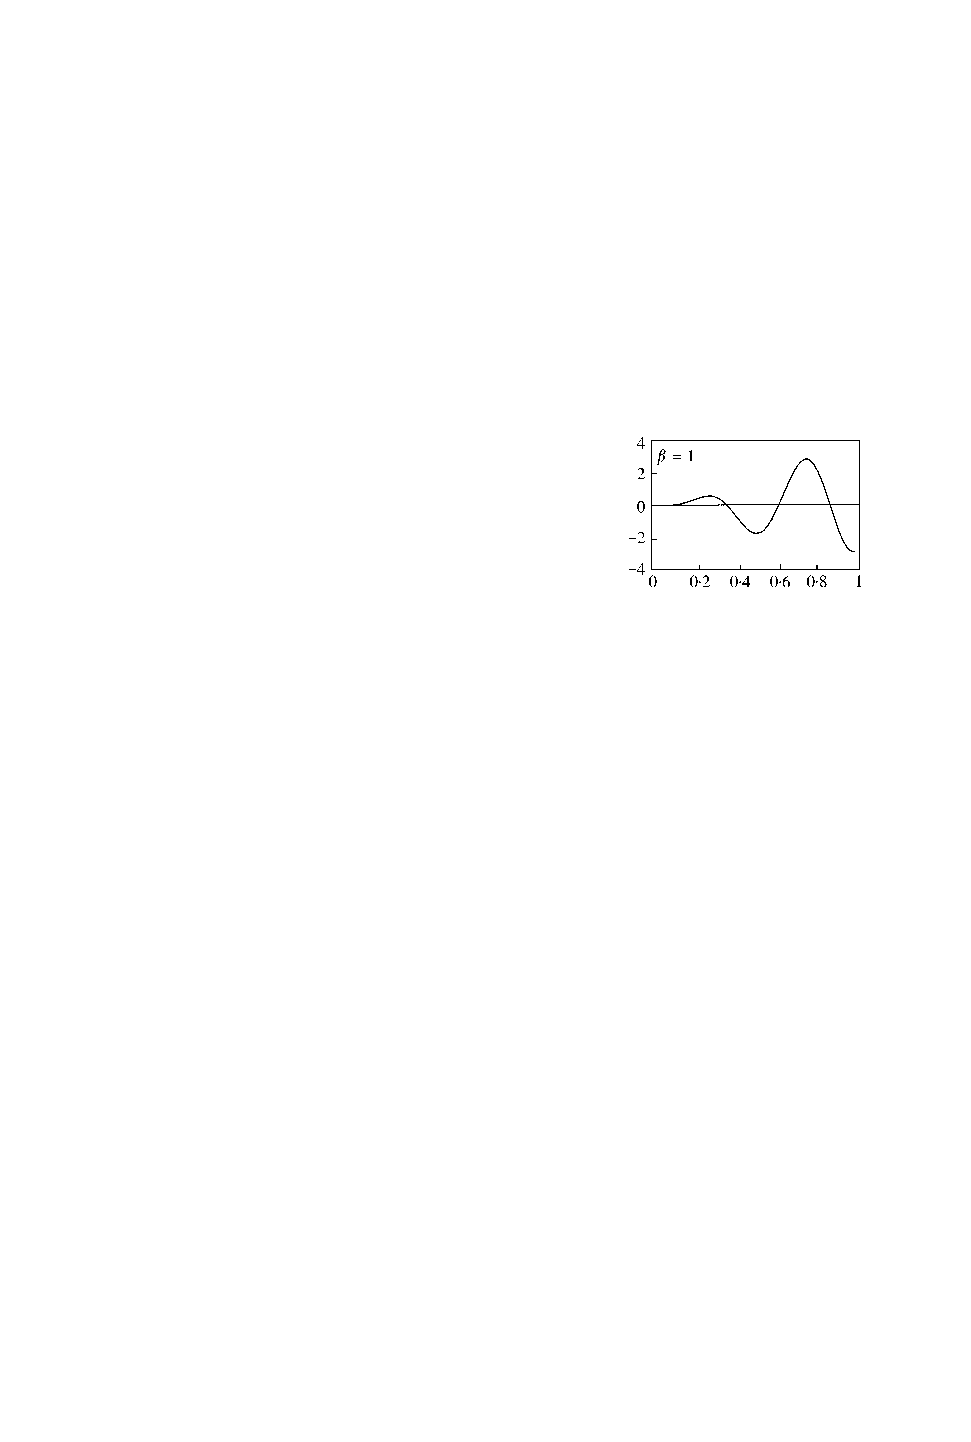
\includegraphics[width=0.5\textwidth]{hilalplot}
    \caption{Reference plot extracted from \citet{abu2000vibration}. Condition: $\alpha = 0.25$, $\zeta = 0.05$, $\beta  = 1$. Y axis for dynamic amplification factor.}
    \label{fig:hilalplot}
\end{figure}

Next step is to translate parameters used in above plot to usable parameters in Eq.\ref{eq:v(x,t)simpleharmonic}.


$$c_{cr} = \frac{\omega_1 L}{\pi} = \frac{\pi}{l}\sqrt{\frac{EJ}{\mu}}$$

$$\alpha = \frac{c}{c_{cr}}$$

$$c = \alpha c_{cr} = \frac{\alpha\pi}{l}\sqrt{\frac{EJ}{\mu}}$$

$EJ$,$\mu$,$l$ needs to be selected to yield value for $c$, thus following values are randomly selected:

$$EJ = 2.43e10 Nm^2$$

$$l = 54m$$

$$\mu = 6000 kg/m$$

$$c_{cr} = 117.05 m/s$$

$$ c = 29.26 m/s $$

A Matlab script is written to automate numerical calculating procedure. By typing 

\texttt{fogtest(2.43e10,54,6000,29.26,0.05)}

into the console. Figure.\ref{fig:EJ24300000000L54mu6000c29daf.tikz} is obtained.

\begin{figure}[h!]
\centering 
\newlength\figureheight 
\newlength\figurewidth 
\setlength\figureheight{6cm} 
\setlength\figurewidth{6cm} 
% This file was created by matlab2tikz v0.4.7 (commit 949a076472a7bec3ddc3d4cd9cc5273c97709f91) running on MATLAB 8.3.
% Copyright (c) 2008--2014, Nico Schlmer <nico.schloemer@gmail.com>
% All rights reserved.
% Minimal pgfplots version: 1.3
% 
\begin{tikzpicture}

\begin{axis}[%
width=\figurewidth,
height=\figureheight,
scale only axis,
xmin=0,
xmax=2,
ymin=-4,
ymax=4
]
\addplot [color=blue,solid,forget plot]
  table[row sep=crcr]{%
0	0\\
0.00186206896551724	-9.81557918731428e-06\\
0.00372413793103448	-3.92485973868528e-05\\
0.00558620689655172	-8.82641320004888e-05\\
0.00744827586206897	-0.000156808154525201\\
0.00931034482758621	-0.000244807560818895\\
0.0111724137931034	-0.000352170209420864\\
0.0130344827586207	-0.000478784967915698\\
0.0148965517241379	-0.000624521767319481\\
0.0167586206896552	-0.000789231664470319\\
0.0186206896551724	-0.000972746912398953\\
0.0204827586206897	-0.00117488103865367\\
0.0223448275862069	-0.00139542893155333\\
0.0242068965517241	-0.0016341669343347\\
0.0260689655172414	-0.0018908529471638\\
0.0279310344827586	-0.00216522653697387\\
0.0297931034482759	-0.00245700905508991\\
0.0316551724137931	-0.00276590376260297\\
0.0335172413793103	-0.00309159596344666\\
0.0353793103448276	-0.00343375314513037\\
0.0372413793103448	-0.00379202512708536\\
0.0391034482758621	-0.00416604421656322\\
0.0409655172413793	-0.00455542537204366\\
0.0428275862068965	-0.0049597663740878\\
0.0446896551724138	-0.00537864800358338\\
0.046551724137931	-0.00581163422731614\\
0.0484137931034483	-0.0062582723908105\\
0.0502758620689655	-0.00671809341836777\\
0.0521379310344828	-0.00719061202023671\\
0.054	-0.00767532690684718\\
0.0558620689655172	-0.00817172101002975\\
0.0577241379310345	-0.0086792617111522\\
0.0595862068965517	-0.00919740107609054\\
0.061448275862069	-0.00972557609695757\\
0.0633103448275862	-0.0102632089405056\\
0.0651724137931034	-0.0108097072031222\\
0.0670344827586207	-0.0113644641723273\\
0.0688965517241379	-0.0119268590946905\\
0.0707586206896552	-0.0124962574500712\\
0.0726206896551724	-0.0130720112320935\\
0.0744827586206896	-0.0136534592347589\\
0.0763448275862069	-0.0142399273451013\\
0.0782068965517241	-0.0148307288417832\\
0.0800689655172414	-0.0154251646995372\\
0.0819310344827586	-0.0160225238993431\\
0.0837931034482759	-0.0166220837442425\\
0.0856551724137931	-0.0172231101806802\\
0.0875172413793103	-0.0178248581252654\\
0.0893793103448276	-0.0184265717968423\\
0.0912413793103448	-0.019027485053758\\
0.0931034482758621	-0.0196268217362131\\
0.0949655172413793	-0.0202237960135815\\
0.0968275862068965	-0.0208176127365785\\
0.0986896551724138	-0.0214074677941622\\
0.100551724137931	-0.0219925484750448\\
0.102413793103448	-0.0225720338336929\\
0.104275862068966	-0.0231450950606914\\
0.106137931034483	-0.0237108958573492\\
0.108	-0.024268592814415\\
0.109862068965517	-0.0248173357947798\\
0.111724137931034	-0.0253562683200327\\
0.113586206896552	-0.0258845279607415\\
0.115448275862069	-0.026401246730324\\
0.117310344827586	-0.0269055514823772\\
0.119172413793103	-0.0273965643113307\\
0.121034482758621	-0.0278734029562845\\
0.122896551724138	-0.0283351812078991\\
0.124758620689655	-0.0287810093181939\\
0.126620689655172	-0.0292099944131192\\
0.12848275862069	-0.0296212409077586\\
0.130344827586207	-0.03001385092402\\
0.132206896551724	-0.0303869247106758\\
0.134068965517241	-0.0307395610656031\\
0.135931034482759	-0.0310708577600861\\
0.137793103448276	-0.0313799119650312\\
0.139655172413793	-0.0316658206789497\\
0.14151724137931	-0.0319276811575626\\
0.143379310344828	-0.0321645913448785\\
0.145241379310345	-0.0323756503055976\\
0.147103448275862	-0.0325599586586926\\
0.148965517241379	-0.0327166190120181\\
0.150827586206897	-0.0328447363977961\\
0.152689655172414	-0.0329434187088317\\
0.154551724137931	-0.0330117771353033\\
0.156413793103448	-0.0330489266019807\\
0.158275862068966	-0.0330539862057153\\
0.160137931034483	-0.0330260796530559\\
0.162	-0.0329643356978319\\
0.163862068965517	-0.0328678885785568\\
0.165724137931034	-0.0327358784554969\\
0.167586206896552	-0.0325674518472536\\
0.169448275862069	-0.0323617620667063\\
0.171310344827586	-0.0321179696561639\\
0.173172413793103	-0.0318352428215708\\
0.175034482758621	-0.0315127578656171\\
0.176896551724138	-0.0311496996195988\\
0.178758620689655	-0.0307452618738761\\
0.180620689655172	-0.030298647806778\\
0.18248275862069	-0.029809070411802\\
0.184344827586207	-0.0292757529229552\\
0.186206896551724	-0.0286979292380885\\
0.188068965517241	-0.0280748443400706\\
0.189931034482759	-0.0274057547156529\\
0.191793103448276	-0.026689928771875\\
0.193655172413793	-0.0259266472498608\\
0.19551724137931	-0.0251152036358579\\
0.197379310344828	-0.0242549045693701\\
0.199241379310345	-0.0233450702482374\\
0.201103448275862	-0.0223850348305153\\
0.202965517241379	-0.0213741468330077\\
0.204827586206897	-0.0203117695263084\\
0.206689655172414	-0.0191972813262065\\
0.208551724137931	-0.0180300761813122\\
0.210413793103448	-0.0168095639567602\\
0.212275862068966	-0.015535170813849\\
0.214137931034483	-0.0142063395854758\\
0.216	-0.012822530147227\\
0.217862068965517	-0.0113832197839859\\
0.219724137931034	-0.0098879035519203\\
0.221586206896552	-0.0083360946357138\\
0.223448275862069	-0.00672732470090573\\
0.225310344827586	-0.00506114424120609\\
0.227172413793103	-0.00333712292065325\\
0.229034482758621	-0.00155484991048313\\
0.230896551724138	0.000286065779419632\\
0.232758620689655	0.00218599497461664\\
0.234620689655172	0.00414528801588362\\
0.23648275862069	0.00616427444477682\\
0.238344827586207	0.00824326269512078\\
0.240206896551724	0.0103825397905403\\
0.242068965517241	0.0125823710481567\\
0.243931034482759	0.0148429997885672\\
0.245793103448276	0.0171646470522243\\
0.247655172413793	0.0195475113223312\\
0.24951724137931	0.0219917682543657\\
0.251379310344828	0.0244975704123454\\
0.253241379310345	0.027065047011943\\
0.255103448275862	0.0296943036705609\\
0.256965517241379	0.0323854221644705\\
0.258827586206897	0.0351384601931194\\
0.260689655172414	0.0379534511507114\\
0.262551724137931	0.0408304039051558\\
0.264413793103448	0.0437693025844865\\
0.266275862068966	0.0467701063708472\\
0.268137931034483	0.0498327493021337\\
0.27	0.0529571400813884\\
0.271862068965517	0.0561431618940342\\
0.273724137931035	0.059390672233036\\
0.275586206896552	0.0626995027320748\\
0.277448275862069	0.0660694590068173\\
0.279310344827586	0.0695003205043603\\
0.281172413793103	0.0729918403609313\\
0.283034482758621	0.076543745267916\\
0.284896551724138	0.0801557353462911\\
0.286758620689655	0.0838274840295311\\
0.288620689655172	0.0875586379550571\\
0.29048275862069	0.0913488168642963\\
0.292344827586207	0.0951976135114118\\
0.294206896551724	0.0991045935807694\\
0.296068965517241	0.103069295613194\\
0.297931034482759	0.107091230941078\\
0.299793103448276	0.111169883632387\\
0.301655172413793	0.115304710443627\\
0.30351724137931	0.119495140781804\\
0.305379310344828	0.123740576675438\\
0.307241379310345	0.128040392754662\\
0.309103448275862	0.13239393624046\\
0.310965517241379	0.136800526943065\\
0.312827586206897	0.141259457269567\\
0.314689655172414	0.145769992240753\\
0.316551724137931	0.150331369517218\\
0.318413793103448	0.154942799434769\\
0.320275862068966	0.159603465049135\\
0.322137931034483	0.164312522190035\\
0.324	0.169069099524586\\
0.325862068965517	0.173872298630094\\
0.327724137931034	0.17872119407623\\
0.329586206896552	0.1836148335166\\
0.331448275862069	0.188552237789721\\
0.333310344827586	0.193532401029408\\
0.335172413793103	0.198554290784571\\
0.337034482758621	0.203616848148417\\
0.338896551724138	0.208718987897069\\
0.340758620689655	0.213859598637574\\
0.342620689655172	0.219037542965308\\
0.34448275862069	0.224251657630757\\
0.346344827586207	0.229500753715663\\
0.348206896551724	0.23478361681851\\
0.350068965517241	0.240099007249341\\
0.351931034482759	0.245445660233871\\
0.353793103448276	0.250822286126875\\
0.355655172413793	0.256227570634824\\
0.35751724137931	0.261660175047732\\
0.359379310344828	0.267118736480177\\
0.361241379310345	0.272601868121471\\
0.363103448275862	0.278108159494919\\
0.364965517241379	0.283636176726144\\
0.366827586206897	0.289184462820415\\
0.368689655172414	0.294751537948938\\
0.370551724137931	0.300335899744058\\
0.372413793103448	0.305936023603311\\
0.374275862068966	0.311550363002279\\
0.376137931034483	0.317177349816177\\
0.378	0.322815394650113\\
0.379862068965517	0.328462887177965\\
0.381724137931034	0.334118196489785\\
0.383586206896552	0.339779671447686\\
0.385448275862069	0.345445641050113\\
0.387310344827586	0.351114414804436\\
0.389172413793103	0.35678428310779\\
0.391034482758621	0.362453517636058\\
0.392896551724138	0.368120371740943\\
0.394758620689655	0.373783080855018\\
0.396620689655172	0.379439862904672\\
0.39848275862069	0.385088918730867\\
0.400344827586207	0.390728432517602\\
0.402206896551724	0.396356572227985\\
0.404068965517241	0.401971490047827\\
0.405931034482759	0.407571322836642\\
0.407793103448276	0.413154192585953\\
0.409655172413793	0.418718206884799\\
0.41151724137931	0.424261459392328\\
0.413379310344828	0.429782030317375\\
0.415241379310345	0.435277986904894\\
0.417103448275862	0.440747383929147\\
0.418965517241379	0.446188264193508\\
0.420827586206897	0.451598659036792\\
0.422689655172414	0.456976588845944\\
0.424551724137931	0.46232006357501\\
0.426413793103448	0.467627083270221\\
0.428275862068966	0.47289563860108\\
0.430137931034483	0.478123711397325\\
0.432	0.483309275191616\\
0.433862068965517	0.488450295767824\\
0.435724137931034	0.49354473171478\\
0.437586206896552	0.498590534985337\\
0.439448275862069	0.503585651460623\\
0.441310344827586	0.508528021519305\\
0.443172413793103	0.513415580611761\\
0.445034482758621	0.518246259838978\\
0.446896551724138	0.523017986536041\\
0.448758620689655	0.527728684860068\\
0.450620689655172	0.532376276382418\\
0.45248275862069	0.536958680685035\\
0.454344827586207	0.541473815960768\\
0.456206896551724	0.545919599617503\\
0.458068965517241	0.550293948885949\\
0.459931034482759	0.554594781430921\\
0.461793103448276	0.558820015965959\\
0.463655172413793	0.562967572871105\\
0.46551724137931	0.567035374813693\\
0.467379310344828	0.571021347371965\\
0.469241379310345	0.574923419661363\\
0.471103448275862	0.578739524963313\\
0.472965517241379	0.582467601356336\\
0.474827586206897	0.586105592349322\\
0.476689655172414	0.589651447516774\\
0.478551724137931	0.59310312313587\\
0.480413793103448	0.596458582825156\\
0.482275862068965	0.599715798184694\\
0.484137931034483	0.602872749437488\\
0.486	0.605927426072021\\
0.487862068965517	0.608877827485703\\
0.489724137931034	0.611721963629069\\
0.491586206896552	0.614457855650545\\
0.493448275862069	0.617083536541579\\
0.495310344827586	0.619597051781993\\
0.497172413793103	0.621996459985335\\
0.499034482758621	0.624279833544076\\
0.500896551724138	0.626445259274457\\
0.502758620689655	0.628490839060793\\
0.504620689655172	0.630414690499073\\
0.50648275862069	0.632214947539652\\
0.508344827586207	0.633889761128852\\
0.510206896551724	0.635437299849293\\
0.512068965517241	0.636855750558771\\
0.513931034482759	0.63814331902748\\
0.515793103448276	0.639298230573417\\
0.517655172413793	0.640318730695758\\
0.51951724137931	0.641203085706045\\
0.521379310344828	0.641949583356971\\
0.523241379310345	0.642556533468602\\
0.525103448275862	0.643022268551835\\
0.526965517241379	0.643345144428911\\
0.528827586206897	0.643523540850792\\
0.530689655172414	0.643555862111235\\
0.532551724137931	0.643440537657353\\
0.534413793103448	0.643176022696495\\
0.536275862068965	0.642760798799259\\
0.538137931034483	0.642193374498452\\
0.54	0.641472285883818\\
0.541862068965517	0.640596097192338\\
0.543724137931034	0.639563401393946\\
0.545586206896552	0.638372820772449\\
0.547448275862069	0.637023007501506\\
0.549310344827586	0.635512644215449\\
0.551172413793103	0.633840444574796\\
0.553034482758621	0.632005153826269\\
0.554896551724138	0.630005549357133\\
0.556758620689655	0.627840441243693\\
0.558620689655172	0.625508672793767\\
0.56048275862069	0.623009121082959\\
0.562344827586207	0.62034069748457\\
0.564206896551724	0.617502348192959\\
0.566068965517241	0.614493054740209\\
0.567931034482759	0.611311834505898\\
0.569793103448276	0.607957741219835\\
0.571655172413793	0.604429865457582\\
0.57351724137931	0.600727335128594\\
0.575379310344828	0.596849315956828\\
0.577241379310345	0.592795011953648\\
0.579103448275862	0.588563665882864\\
0.580965517241379	0.584154559717757\\
0.582827586206897	0.579567015089932\\
0.584689655172414	0.574800393729829\\
0.586551724137931	0.569854097898763\\
0.588413793103448	0.564727570812318\\
0.590275862068966	0.559420297054966\\
0.592137931034483	0.553931802985745\\
0.594	0.548261657134866\\
0.595862068965517	0.542409470591096\\
0.597724137931035	0.536374897379779\\
0.599586206896552	0.530157634831351\\
0.601448275862069	0.523757423940224\\
0.603310344827586	0.51717404971388\\
0.605172413793103	0.510407341512074\\
0.607034482758621	0.503457173375987\\
0.608896551724138	0.496323464347213\\
0.610758620689655	0.489006178776454\\
0.612620689655172	0.481505326621797\\
0.61448275862069	0.473820963736455\\
0.616344827586207	0.465953192145843\\
0.618206896551724	0.457902160313883\\
0.620068965517241	0.449668063398425\\
0.621931034482759	0.441251143495659\\
0.623793103448276	0.432651689873427\\
0.625655172413793	0.42387003919331\\
0.62751724137931	0.414906575721403\\
0.629379310344828	0.405761731527673\\
0.631241379310345	0.396435986673787\\
0.633103448275862	0.386929869389337\\
0.634965517241379	0.377243956236354\\
0.636827586206897	0.367378872262029\\
0.638689655172414	0.357335291139542\\
0.640551724137931	0.347113935296942\\
0.642413793103448	0.336715576033949\\
0.644275862068965	0.326141033626664\\
0.646137931034483	0.315391177420043\\
0.648	0.304466925908124\\
0.649862068965517	0.293369246801887\\
0.651724137931034	0.282099157084721\\
0.653586206896552	0.270657723055406\\
0.655448275862069	0.259046060358566\\
0.657310344827586	0.247265334002526\\
0.659172413793103	0.235316758364535\\
0.661034482758621	0.223201597183277\\
0.662896551724138	0.210921163538648\\
0.664758620689655	0.198476819818751\\
0.666620689655172	0.185869977674043\\
0.66848275862069	0.173102097958634\\
0.670344827586207	0.160174690658672\\
0.672206896551724	0.147089314807804\\
0.674068965517241	0.133847578389661\\
0.675931034482759	0.120451138227375\\
0.677793103448276	0.10690169986007\\
0.679655172413793	0.0932010174063413\\
0.68151724137931	0.079350893414683\\
0.683379310344828	0.0653531787008695\\
0.685241379310345	0.0512097721722685\\
0.687103448275862	0.0369226206390988\\
0.688965517241379	0.0224937186126111\\
0.690827586206897	0.00792510809020755\\
0.692689655172414	-0.00678112167249782\\
0.694551724137931	-0.021622834402677\\
0.696413793103448	-0.0365978470643081\\
0.698275862068966	-0.0517039301252449\\
0.700137931034483	-0.0669388078372642\\
0.702	-0.0823001585291173\\
0.703862068965517	-0.0977856149125212\\
0.705724137931035	-0.113392764401088\\
0.707586206896552	-0.129119149442143\\
0.709448275862069	-0.144962267861408\\
0.711310344827586	-0.160919573220491\\
0.713172413793103	-0.176988475187163\\
0.715034482758621	-0.193166339918363\\
0.716896551724138	-0.209450490455876\\
0.718758620689655	-0.225838207134646\\
0.720620689655172	-0.242326728003651\\
0.72248275862069	-0.258913249259291\\
0.724344827586207	-0.275594925691231\\
0.726206896551724	-0.292368871140608\\
0.728068965517241	-0.309232158970556\\
0.729931034482759	-0.326181822548973\\
0.731793103448276	-0.343214855743434\\
0.733655172413793	-0.360328213428194\\
0.73551724137931	-0.377518812003182\\
0.737379310344828	-0.394783529924907\\
0.739241379310345	-0.412119208249166\\
0.741103448275862	-0.429522651185513\\
0.742965517241379	-0.446990626663316\\
0.744827586206897	-0.464519866909372\\
0.746689655172414	-0.482107069036923\\
0.748551724137931	-0.499748895646021\\
0.750413793103448	-0.51744197543507\\
0.752275862068966	-0.535182903823492\\
0.754137931034483	-0.552968243585347\\
0.756	-0.570794525493843\\
0.757862068965517	-0.588658248976563\\
0.759724137931034	-0.606555882781318\\
0.761586206896552	-0.624483865652484\\
0.763448275862069	-0.64243860701768\\
0.765310344827586	-0.660416487684699\\
0.767172413793103	-0.678413860548483\\
0.769034482758621	-0.696427051308071\\
0.770896551724138	-0.714452359193322\\
0.772758620689655	-0.732486057701319\\
0.774620689655172	-0.750524395342251\\
0.77648275862069	-0.768563596394667\\
0.778344827586207	-0.786599861669912\\
0.780206896551724	-0.80462936928562\\
0.782068965517241	-0.822648275448076\\
0.783931034482759	-0.840652715243304\\
0.785793103448276	-0.858638803436699\\
0.787655172413793	-0.876602635281054\\
0.78951724137931	-0.894540287332788\\
0.791379310344828	-0.912447818276233\\
0.793241379310345	-0.930321269755765\\
0.795103448275862	-0.948156667215639\\
0.796965517241379	-0.96595002074732\\
0.798827586206897	-0.983697325944142\\
0.800689655172414	-1.00139456476311\\
0.802551724137931	-1.01903770639363\\
0.804413793103448	-1.03662270813303\\
0.806275862068966	-1.05414551626864\\
0.808137931034483	-1.07160206696622\\
0.81	-1.08898828716459\\
0.811862068965517	-1.10630009547625\\
0.813724137931034	-1.12353340309376\\
0.815586206896552	-1.14068411470167\\
0.817448275862069	-1.15774812939389\\
0.819310344827586	-1.17472134159613\\
0.821172413793103	-1.19159964199341\\
0.823034482758621	-1.2083789184622\\
0.824896551724138	-1.22505505700717\\
0.826758620689655	-1.24162394270226\\
0.828620689655172	-1.25808146063576\\
0.83048275862069	-1.27442349685944\\
0.832344827586207	-1.29064593934118\\
0.834206896551724	-1.30674467892118\\
0.836068965517241	-1.32271561027131\\
0.837931034482759	-1.33855463285751\\
0.839793103448276	-1.35425765190498\\
0.841655172413793	-1.36982057936584\\
0.84351724137931	-1.38523933488926\\
0.845379310344828	-1.40050984679354\\
0.847241379310345	-1.41562805304017\\
0.849103448275862	-1.43058990220948\\
0.850965517241379	-1.4453913544777\\
0.852827586206897	-1.46002838259521\\
0.854689655172414	-1.47449697286571\\
0.856551724137931	-1.48879312612616\\
0.858413793103448	-1.50291285872708\\
0.860275862068966	-1.51685220351325\\
0.862137931034483	-1.53060721080421\\
0.864	-1.54417394937472\\
0.865862068965517	-1.55754850743462\\
0.867724137931035	-1.57072699360804\\
0.869586206896552	-1.58370553791162\\
0.871448275862069	-1.59648029273158\\
0.873310344827586	-1.60904743379932\\
0.875172413793103	-1.62140316116541\\
0.877034482758621	-1.63354370017161\\
0.878896551724138	-1.64546530242077\\
0.880758620689655	-1.65716424674438\\
0.882620689655172	-1.6686368401674\\
0.88448275862069	-1.67987941887032\\
0.886344827586207	-1.69088834914804\\
0.888206896551724	-1.70166002836545\\
0.890068965517241	-1.7121908859094\\
0.891931034482759	-1.7224773841368\\
0.893793103448276	-1.73251601931877\\
0.895655172413793	-1.74230332258036\\
0.89751724137931	-1.75183586083578\\
0.899379310344828	-1.76111023771883\\
0.901241379310345	-1.77012309450837\\
0.903103448275862	-1.77887111104844\\
0.904965517241379	-1.78735100666293\\
0.906827586206897	-1.79555954106455\\
0.908689655172414	-1.80349351525777\\
0.910551724137931	-1.81114977243564\\
0.912413793103448	-1.81852519887012\\
0.914275862068965	-1.82561672479576\\
0.916137931034483	-1.83242132528648\\
0.918	-1.83893602112529\\
0.919862068965517	-1.84515787966654\\
0.921724137931034	-1.85108401569071\\
0.923586206896552	-1.85671159225129\\
0.925448275862069	-1.86203782151373\\
0.927310344827586	-1.86705996558604\\
0.929172413793103	-1.87177533734095\\
0.931034482758621	-1.87618130122941\\
0.932896551724138	-1.88027527408512\\
0.934758620689655	-1.88405472591992\\
0.936620689655172	-1.88751718070989\\
0.93848275862069	-1.89066021717181\\
0.940344827586207	-1.89348146952989\\
0.942206896551724	-1.8959786282725\\
0.944068965517241	-1.89814944089869\\
0.945931034482759	-1.89999171265432\\
0.947793103448276	-1.90150330725756\\
0.949655172413793	-1.90268214761362\\
0.95151724137931	-1.90352621651842\\
0.953379310344827	-1.90403355735105\\
0.955241379310345	-1.90420227475488\\
0.957103448275862	-1.90403053530698\\
0.958965517241379	-1.90351656817583\\
0.960827586206896	-1.90265866576697\\
0.962689655172414	-1.90145518435654\\
0.964551724137931	-1.89990454471246\\
0.966413793103448	-1.89800523270297\\
0.968275862068965	-1.89575579989265\\
0.970137931034483	-1.89315486412533\\
0.972	-1.89020111009409\\
0.973862068965517	-1.88689328989794\\
0.975724137931034	-1.88323022358511\\
0.977586206896552	-1.87921079968277\\
0.979448275862069	-1.87483397571303\\
0.981310344827586	-1.87009877869496\\
0.983172413793103	-1.86500430563268\\
0.985034482758621	-1.85954972398914\\
0.986896551724138	-1.85373427214557\\
0.988758620689655	-1.8475572598464\\
0.990620689655172	-1.84101806862959\\
0.99248275862069	-1.83411615224208\\
0.994344827586207	-1.82685103704035\\
0.996206896551724	-1.81922232237589\\
0.998068965517241	-1.81122968096549\\
0.999931034482759	-1.80287285924615\\
1.00179310344828	-1.79415167771457\\
1.00365517241379	-1.78506603125105\\
1.00551724137931	-1.77561588942767\\
1.00737931034483	-1.7658012968007\\
1.00924137931034	-1.75562237318698\\
1.01110344827586	-1.74507931392443\\
1.01296551724138	-1.73417239011622\\
1.0148275862069	-1.72290194885885\\
1.01668965517241	-1.71126841345382\\
1.01855172413793	-1.69927228360288\\
1.02041379310345	-1.68691413558676\\
1.02227586206897	-1.67419462242723\\
1.02413793103448	-1.66111447403259\\
1.026	-1.64767449732623\\
1.02786206896552	-1.63387557635847\\
1.02972413793103	-1.6197186724014\\
1.03158620689655	-1.60520482402676\\
1.03344827586207	-1.59033514716674\\
1.03531034482759	-1.57511083515772\\
1.0371724137931	-1.55953315876676\\
1.03903448275862	-1.54360346620095\\
1.04089655172414	-1.52732318309944\\
1.04275862068966	-1.51069381250813\\
1.04462068965517	-1.49371693483709\\
1.04648275862069	-1.4763942078005\\
1.04834482758621	-1.4587273663392\\
1.05020689655172	-1.44071822252582\\
1.05206896551724	-1.42236866545236\\
1.05393103448276	-1.40368066110033\\
1.05579310344828	-1.38465625219338\\
1.05765517241379	-1.36529755803233\\
1.05951724137931	-1.34560677431276\\
1.06137931034483	-1.32558617292503\\
1.06324137931034	-1.30523810173669\\
1.06510344827586	-1.2845649843575\\
1.06696551724138	-1.26356931988678\\
1.0688275862069	-1.24225368264335\\
1.07068965517241	-1.22062072187791\\
1.07255172413793	-1.198673161468\\
1.07441379310345	-1.17641379959545\\
1.07627586206897	-1.15384550840647\\
1.07813793103448	-1.1309712336543\\
1.08	-1.10779399432453\\
1.08186206896552	-1.08431688224316\\
1.08372413793103	-1.06054306166728\\
1.08558620689655	-1.03647576885867\\
1.08744827586207	-1.01211831164013\\
1.08931034482759	-0.987474068934819\\
1.0911724137931	-0.962546490288424\\
1.09303448275862	-0.937339095374474\\
1.09489655172414	-0.911855473482685\\
1.09675862068966	-0.886099282990505\\
1.09862068965517	-0.860074250817898\\
1.10048275862069	-0.833784171865461\\
1.10234482758621	-0.807232908435964\\
1.10420689655172	-0.78042438963941\\
1.10606896551724	-0.753362610781681\\
1.10793103448276	-0.726051632736905\\
1.10979310344828	-0.698495581303635\\
1.11165517241379	-0.670698646544895\\
1.11351724137931	-0.642665082112342\\
1.11537931034483	-0.614399204554451\\
1.11724137931034	-0.585905392609072\\
1.11910344827586	-0.55718808648028\\
1.12096551724138	-0.528251787099785\\
1.1228275862069	-0.499101055372936\\
1.12468965517241	-0.469740511409543\\
1.12655172413793	-0.440174833739573\\
1.12841379310345	-0.410408758513911\\
1.13027586206897	-0.38044707869031\\
1.13213793103448	-0.350294643204681\\
1.134	-0.319956356127899\\
1.13586206896552	-0.289437175808249\\
1.13772413793103	-0.258742113999691\\
1.13958620689655	-0.227876234976094\\
1.14144827586207	-0.196844654631626\\
1.14331034482759	-0.165652539567445\\
1.1451724137931	-0.134305106164915\\
1.14703448275862	-0.102807619645439\\
1.14889655172414	-0.0711653931171906\\
1.15075862068965	-0.0393837866088264\\
1.15262068965517	-0.00746820609047376\\
1.15448275862069	0.0245758975179002\\
1.15634482758621	0.0567430293505014\\
1.15820689655172	0.0890276516119292\\
1.16006896551724	0.121424184605382\\
1.16193103448276	0.153927007772639\\
1.16379310344828	0.18653046074566\\
1.16565517241379	0.219228844409508\\
1.16751724137931	0.252016421976482\\
1.16937931034483	0.284887420071166\\
1.17124137931034	0.317836029826191\\
1.17310344827586	0.350856407988532\\
1.17496551724138	0.383942678036045\\
1.1768275862069	0.417088931304075\\
1.17868965517241	0.450289228121873\\
1.18055172413793	0.483537598958629\\
1.18241379310345	0.516828045578793\\
1.18427586206897	0.550154542206551\\
1.18613793103448	0.583511036699169\\
1.188	0.61689145172896\\
1.18986206896552	0.650289685973619\\
1.19172413793103	0.683699615314713\\
1.19358620689655	0.717115094044015\\
1.19544827586207	0.75052995607753\\
1.19731034482759	0.783938016176824\\
1.1991724137931	0.817333071177532\\
1.20103448275862	0.85070890122469\\
1.20289655172414	0.88405927101465\\
1.20475862068966	0.917377931043391\\
1.20662068965517	0.950658618860812\\
1.20848275862069	0.98389506033091\\
1.21034482758621	1.01708097089743\\
1.21220689655172	1.05021005685482\\
1.21406896551724	1.08327601662411\\
1.21593103448276	1.11627254203361\\
1.21779310344828	1.14919331960395\\
1.21965517241379	1.18203203183734\\
1.22151724137931	1.21478235851071\\
1.22337931034483	1.2474379779724\\
1.22524137931034	1.27999256844227\\
1.22710344827586	1.31243980931476\\
1.22896551724138	1.34477338246478\\
1.2308275862069	1.37698697355603\\
1.23268965517241	1.40907427335151\\
1.23455172413793	1.44102897902596\\
1.23641379310345	1.47284479547986\\
1.23827586206897	1.50451543665486\\
1.24013793103448	1.53603462685009\\
1.242	1.56739610203938\\
1.24386206896552	1.59859361118881\\
1.24572413793103	1.6296209175745\\
1.24758620689655	1.66047180010024\\
1.24944827586207	1.69114005461471\\
1.25131034482759	1.72161949522796\\
1.2531724137931	1.75190395562694\\
1.25503448275862	1.78198729038971\\
1.25689655172414	1.81186337629802\\
1.25875862068966	1.84152611364805\\
1.26062068965517	1.87096942755897\\
1.26248275862069	1.90018726927899\\
1.26434482758621	1.92917361748869\\
1.26620689655172	1.95792247960128\\
1.26806896551724	1.98642789305949\\
1.26993103448276	2.01468392662882\\
1.27179310344828	2.04268468168686\\
1.27365517241379	2.0704242935084\\
1.27551724137931	2.09789693254601\\
1.27737931034483	2.12509680570574\\
1.27924137931034	2.15201815761788\\
1.28110344827586	2.17865527190213\\
1.28296551724138	2.20500247242724\\
1.2848275862069	2.23105412456465\\
1.28668965517241	2.25680463643582\\
1.28855172413793	2.28224846015307\\
1.29041379310345	2.3073800930536\\
1.29227586206897	2.33219407892636\\
1.29413793103448	2.35668500923155\\
1.296	2.3808475243125\\
1.29786206896552	2.40467631459945\\
1.29972413793103	2.42816612180528\\
1.30158620689655	2.45131174011258\\
1.30344827586207	2.47410801735204\\
1.30531034482759	2.49654985617168\\
1.3071724137931	2.51863221519687\\
1.30903448275862	2.54035011018061\\
1.31089655172414	2.56169861514405\\
1.31275862068966	2.5826728635068\\
1.31462068965517	2.60326804920689\\
1.31648275862069	2.62347942780997\\
1.31834482758621	2.64330231760768\\
1.32020689655172	2.6627321007048\\
1.32206896551724	2.68176422409489\\
1.32393103448276	2.70039420072433\\
1.32579310344828	2.71861761054428\\
1.32765517241379	2.73643010155058\\
1.32951724137931	2.7538273908111\\
1.33137931034483	2.77080526548037\\
1.33324137931034	2.78735958380135\\
1.33510344827586	2.80348627609396\\
1.33696551724138	2.81918134573023\\
1.3388275862069	2.83444087009571\\
1.34068965517241	2.84926100153711\\
1.34255172413793	2.86363796829571\\
1.34441379310345	2.87756807542654\\
1.34627586206897	2.89104770570286\\
1.34813793103448	2.90407332050594\\
1.35	2.91664146069982\\
1.35186206896552	2.92874874749085\\
1.35372413793103	2.94039188327174\\
1.35558620689655	2.95156765245004\\
1.35744827586207	2.96227292226073\\
1.35931034482759	2.97250464356278\\
1.3611724137931	2.98225985161945\\
1.36303448275862	2.99153566686216\\
1.36489655172414	3.00032929563768\\
1.36675862068966	3.00863803093857\\
1.36862068965517	3.01645925311657\\
1.37048275862069	3.02379043057877\\
1.37234482758621	3.03062912046646\\
1.37420689655172	3.03697296931646\\
1.37606896551724	3.04281971370463\\
1.37793103448276	3.04816718087165\\
1.37979310344828	3.05301328933062\\
1.38165517241379	3.05735604945658\\
1.38351724137931	3.06119356405757\\
1.38537931034483	3.06452402892729\\
1.38724137931034	3.06734573337898\\
1.38910344827586	3.06965706076065\\
1.39096551724138	3.07145648895127\\
1.3928275862069	3.0727425908379\\
1.39468965517241	3.07351403477369\\
1.39655172413793	3.07376958501649\\
1.39841379310345	3.07350810214801\\
1.40027586206897	3.07272854347342\\
1.40213793103448	3.07142996340134\\
1.404	3.0696115138039\\
1.40586206896552	3.06727244435701\\
1.40772413793103	3.06441210286063\\
1.40958620689655	3.06102993553884\\
1.41144827586207	3.05712548731988\\
1.41331034482759	3.05269840209576\\
1.4151724137931	3.04774842296163\\
1.41703448275862	3.04227539243464\\
1.41889655172414	3.0362792526523\\
1.42075862068966	3.0297600455503\\
1.42262068965517	3.0227179130196\\
1.42448275862069	3.01515309704288\\
1.42634482758621	3.00706593981022\\
1.42820689655172	2.99845688381388\\
1.43006896551724	2.98932647192233\\
1.43193103448276	2.9796753474333\\
1.43379310344828	2.96950425410585\\
1.43565517241379	2.95881403617157\\
1.43751724137931	2.94760563832466\\
1.43937931034483	2.93588010569106\\
1.44124137931034	2.92363858377641\\
1.44310344827586	2.91088231839311\\
1.44496551724138	2.89761265556616\\
1.4468275862069	2.88383104141794\\
1.44868965517241	2.86953902203197\\
1.45055172413793	2.85473824329555\\
1.45241379310345	2.83943045072127\\
1.45427586206897	2.82361748924756\\
1.45613793103448	2.80730130301815\\
1.458	2.79048393514046\\
1.45986206896552	2.77316752742312\\
1.46172413793103	2.75535432009242\\
1.46358620689655	2.73704665148785\\
1.46544827586207	2.71824695773687\\
1.46731034482759	2.69895777240865\\
1.4691724137931	2.67918172614723\\
1.47103448275862	2.65892154628378\\
1.47289655172414	2.63818005642833\\
1.47475862068966	2.61696017604078\\
1.47662068965517	2.59526491998148\\
1.47848275862069	2.57309739804124\\
1.48034482758621	2.55046081445104\\
1.48220689655172	2.52735846737145\\
1.48406896551724	2.50379374836176\\
1.48593103448276	2.47977014182907\\
1.48779310344828	2.4552912244573\\
1.48965517241379	2.43036066461634\\
1.49151724137931	2.40498222175134\\
1.49337931034483	2.37915974575235\\
1.49524137931034	2.35289717630426\\
1.49710344827586	2.32619854221745\\
1.49896551724138	2.29906796073892\\
1.5008275862069	2.27150963684433\\
1.50268965517241	2.24352786251089\\
1.50455172413793	2.21512701597134\\
1.50641379310345	2.18631156094911\\
1.50827586206897	2.15708604587483\\
1.51013793103448	2.12745510308432\\
1.512	2.09742344799826\\
1.51386206896552	2.06699587828364\\
1.51572413793103	2.03617727299715\\
1.51758620689655	2.0049725917108\\
1.51944827586207	1.97338687361971\\
1.52131034482759	1.94142523663254\\
1.5231724137931	1.90909287644444\\
1.52503448275862	1.87639506559295\\
1.52689655172414	1.84333715249682\\
1.52875862068966	1.80992456047818\\
1.53062068965517	1.77616278676804\\
1.53248275862069	1.74205740149544\\
1.53434482758621	1.70761404666037\\
1.53620689655172	1.67283843509083\\
1.53806896551724	1.63773634938397\\
1.53993103448276	1.60231364083181\\
1.54179310344828	1.56657622833155\\
1.54365517241379	1.5305300972808\\
1.54551724137931	1.49418129845791\\
1.54737931034483	1.45753594688764\\
1.54924137931034	1.42060022069238\\
1.55110344827586	1.38338035992923\\
1.55296551724138	1.34588266541308\\
1.5548275862069	1.30811349752595\\
1.55668965517241	1.27007927501297\\
1.55855172413793	1.23178647376492\\
1.56041379310345	1.1932416255881\\
1.56227586206897	1.15445131696118\\
1.56413793103448	1.11542218777982\\
1.566	1.0761609300889\\
1.56786206896552	1.03667428680298\\
1.56972413793103	0.996969050414972\\
1.57158620689655	0.957052061693447\\
1.57344827586207	0.916930208368785\\
1.57531034482759	0.876610423808494\\
1.5771724137931	0.836099685681924\\
1.57903448275862	0.795405014614693\\
1.58089655172414	0.754533472833041\\
1.58275862068966	0.713492162798518\\
1.58462068965517	0.672288225833134\\
1.58648275862069	0.630928840735399\\
1.58834482758621	0.589421222387485\\
1.59020689655172	0.547772620353747\\
1.59206896551724	0.505990317471045\\
1.59393103448276	0.464081628430972\\
1.59579310344828	0.422053898354493\\
1.59765517241379	0.379914501359069\\
1.59951724137931	0.337670839118835\\
1.60137931034483	0.295330339417868\\
1.60324137931034	0.252900454697023\\
1.60510344827586	0.210388660594604\\
1.60696551724138	0.167802454481152\\
1.6088275862069	0.125149353988706\\
1.61068965517241	0.0824368955347899\\
1.61255172413793	0.0396726328414738\\
1.61441379310345	-0.00313586455014921\\
1.61627586206897	-0.0459810127698149\\
1.61813793103448	-0.0888552151118905\\
1.62	-0.131750863532865\\
1.62186206896552	-0.174660340152219\\
1.62372413793103	-0.217576018756199\\
1.62558620689655	-0.260490266304447\\
1.62744827586207	-0.303395444438885\\
1.62931034482759	-0.346283910994752\\
1.6311724137931	-0.389148021513328\\
1.63303448275862	-0.431980130756066\\
1.63489655172414	-0.47477259421984\\
1.63675862068966	-0.517517769652992\\
1.63862068965517	-0.5602080185717\\
1.64048275862069	-0.602835707776611\\
1.64234482758621	-0.645393210869144\\
1.64420689655172	-0.68787290976735\\
1.64606896551724	-0.730267196220853\\
1.64793103448276	-0.772568473324615\\
1.64979310344828	-0.814769157031215\\
1.65165517241379	-0.856861677661293\\
1.65351724137931	-0.898838481411805\\
1.65537931034483	-0.940692031861823\\
1.65724137931034	-0.982414811475503\\
1.65910344827586	-1.02399932310194\\
1.66096551724138	-1.06543809147161\\
1.6628275862069	-1.1067236646889\\
1.66468965517241	-1.14784861572074\\
1.66655172413793	-1.18880554388062\\
1.66841379310345	-1.22958707630801\\
1.67027586206897	-1.27018586944265\\
1.67213793103448	-1.31059461049349\\
1.674	-1.35080601890192\\
1.67586206896552	-1.39081284779905\\
1.67772413793103	-1.43060788545653\\
1.67958620689655	-1.47018395673094\\
1.68144827586207	-1.50953392450099\\
1.68331034482759	-1.54865069109771\\
1.6851724137931	-1.58752719972684\\
1.68703448275862	-1.62615643588352\\
1.68889655172414	-1.66453142875869\\
1.69075862068966	-1.70264525263706\\
1.69262068965517	-1.74049102828627\\
1.69448275862069	-1.77806192433695\\
1.69634482758621	-1.81535115865342\\
1.69820689655172	-1.85235199969466\\
1.70006896551724	-1.88905776786537\\
1.70193103448276	-1.92546183685665\\
1.70379310344828	-1.96155763497626\\
1.70565517241379	-1.99733864646787\\
1.70751724137931	-2.03279841281928\\
1.70937931034483	-2.06793053405921\\
1.71124137931034	-2.10272867004232\\
1.71310344827586	-2.13718654172233\\
1.71496551724138	-2.17129793241282\\
1.7168275862069	-2.20505668903552\\
1.71868965517241	-2.23845672335581\\
1.72055172413793	-2.27149201320515\\
1.72241379310345	-2.30415660369013\\
1.72427586206897	-2.33644460838801\\
1.72613793103448	-2.36835021052827\\
1.728	-2.3998676641602\\
1.72986206896552	-2.43099129530599\\
1.73172413793103	-2.46171550309931\\
1.73358620689655	-2.49203476090891\\
1.73544827586207	-2.52194361744722\\
1.73731034482759	-2.55143669786355\\
1.7391724137931	-2.58050870482167\\
1.74103448275862	-2.60915441956166\\
1.74289655172414	-2.63736870294562\\
1.74475862068966	-2.66514649648711\\
1.74662068965517	-2.69248282336419\\
1.74848275862069	-2.71937278941559\\
1.75034482758621	-2.74581158412003\\
1.75220689655172	-2.77179448155841\\
1.75406896551724	-2.79731684135852\\
1.75593103448276	-2.82237410962239\\
1.75779310344828	-2.84696181983562\\
1.75965517241379	-2.87107559375896\\
1.76151724137931	-2.89471114230165\\
1.76337931034483	-2.91786426637638\\
1.76524137931034	-2.94053085773578\\
1.76710344827586	-2.96270689979017\\
1.76896551724138	-2.98438846840641\\
1.7708275862069	-3.00557173268775\\
1.77268965517241	-3.02625295573431\\
1.77455172413793	-3.04642849538433\\
1.77641379310345	-3.06609480493576\\
1.77827586206897	-3.08524843384816\\
1.78013793103448	-3.10388602842476\\
1.782	-3.12200433247443\\
1.78386206896552	-3.13960018795364\\
1.78572413793103	-3.15667053558795\\
1.78758620689655	-3.17321241547324\\
1.78944827586207	-3.18922296765625\\
1.79131034482759	-3.2046994326945\\
1.7931724137931	-3.21963915219543\\
1.79503448275862	-3.23403956933457\\
1.79689655172414	-3.2478982293527\\
1.79875862068966	-3.26121278003185\\
1.80062068965517	-3.27398097215016\\
1.80248275862069	-3.28620065991525\\
1.80434482758621	-3.29786980137628\\
1.80620689655172	-3.30898645881447\\
1.80806896551724	-3.31954879911196\\
1.80993103448276	-3.32955509409908\\
1.81179310344828	-3.33900372087978\\
1.81365517241379	-3.34789316213535\\
1.81551724137931	-3.35622200640613\\
1.81737931034483	-3.36398894835135\\
1.81924137931034	-3.371192788987\\
1.82110344827586	-3.37783243590154\\
1.82296551724138	-3.38390690344966\\
1.8248275862069	-3.38941531292378\\
1.82668965517241	-3.39435689270347\\
1.82855172413793	-3.39873097838265\\
1.83041379310345	-3.40253701287454\\
1.83227586206897	-3.40577454649439\\
1.83413793103448	-3.40844323701999\\
1.836	-3.41054284972983\\
1.83786206896552	-3.41207325741903\\
1.83972413793103	-3.41303444039307\\
1.84158620689655	-3.41342648643908\\
1.84344827586207	-3.41324959077505\\
1.84531034482759	-3.4125040559767\\
1.8471724137931	-3.41119029188209\\
1.84903448275862	-3.40930881547414\\
1.85089655172414	-3.4068602507409\\
1.85275862068966	-3.40384532851367\\
1.85462068965517	-3.40026488628306\\
1.85648275862069	-3.39611986799301\\
1.85834482758621	-3.39141132381271\\
1.86020689655172	-3.38614040988669\\
1.86206896551724	-3.3803083880629\\
};
\end{axis}
\end{tikzpicture}% 
\caption{Time history of dynamic amplification factor in mid-span of the beam. Parameters:$EJ=2.43e10Nm^2$,$L=54m$,$\mu=6000kg/m$,$c=29.26m/s$} 
\label{fig:EJ24300000000L54mu6000c29daf.tikz} 
\end{figure}

By observing Figure.\ref{fig:hilalplot} and Figure.\ref{fig:EJ24300000000L54mu6000c29daf.tikz} it can be concluded that results are the same on y-axis. The difference of x-axis is because in Figure.\ref{fig:hilalplot} time axis is scaled to 1 but in Figure.\ref{fig:EJ24300000000L54mu6000c29daf.tikz} time is not scaled. Then it can be further concluded that Eq.\ref{eq:v(x,t)simpleharmonic} and expression for $\omega_b$ are both correct.


\chapter{New practical method for checking lateral resonance response of railway bridges based on VAMPIRE simulation results }\label{sec:parcticalmethod}

\section{Introduction}

This chapter proposes a new method for checking lateral resonance response of railway bridges. This method aims to provide an engineering solution for checking the deflection and acceleration of railway bridges when resonance happens under horizontal dynamic train load. Both creation and verification of the method is based on VAMPIRE simulation results provided in DT329 research.

The method features the combined usage of a simplified analytical structural model and a more refined lateral force model. The analytical structure model simulates a perfect resonance scenario for railway bridge. And the refined load model, which is a concentrated harmonic moving load, represents the lateral dynamic effects that occur because of the passing of the train. The combination of these two analytical elements will generate a resonance response conservative compared to the simulation output in DT329 because various types of disturbance were included in these simulation runs.

The analytical structural model that was introduced in the previous chapter and its explicit solution has already been worked out in the same chapter. Thus the main objective of this chapter is finding a better lateral force load model because current existing ones are too conservative(see Section.\ref{sec:refinedloadmodel}). The refined load model shall be able to be adopted universally for all regular train types. Once this load model is obtained and verified, it is then possible to take advantage of the combination of the load model and analytical solution for practical designing purposes.

\section{Overview of this chapter}

To give a clear overview of this chapter, procedure of development of the method  as following:

\begin{enumerate}
    \item \textit{Developing:} Develop a more practical load model to be used in pair with the analytical model introduced in previous chapter based on the VAMPIRE simulation outputs. See Section.\ref{sec:refinedloadmodel}
        \begin{enumerate}[label*=\arabic*.]
            \item Overview of both VAMPIRE numerical simulation method and analytical method. See Section.\ref{sec:overviewvampireanalytical}
            \item Find the analytical equivalent nosing forces amplitude for freight trains in 3 different cases presented in DT329 resonance research simulation. See Section.\ref{sec:findingequivalentamplitude}
            \item Find regular pattern and key parameter for the magnitude of nosing forces amplitude for freight trains. See Section.\ref{sec:keyparameterforequivalentamplitudeandhypothesis}
            \item Develop a conservative load model based on observed pattern of nosing force of freight trains. See Section.\ref{sec:keyparameterforequivalentamplitudeandhypothesis}
        \end{enumerate} 
    \item \textit{Verifying:} Validate the feasibility of combined usage of conservative load model and analytical model
        % \begin{enumerate}[label*=\arabic*.]
        %     \item What 
        % \end{enumerate}
    \item \textit{Finalizing:} Illustrate the usage of the method by applying it on a real railway bridge
\end{enumerate}

\begin{figure}[h!]
\centering
\begin{tikzpicture}[node distance=1cm, auto,]
    \node[punkt] (set1) {VAMPIRE simulation results inventory 1};
    \node[punkt, inner sep=15pt,right=2cm of set1]
        (am) {Analytical Method:Explicit solution and equivalent load amplitude};
    \node[punkt, right=2cm of am] (set2) {VAMPIRE simulation results inventory 2};
    \draw[->] (set1) to (am);
    \draw[->] (set2) to (am);
    \node[right=0.8cm of set1] (dummy1) {};
    \node[above=0.1cm of dummy1] (creation) {creation};
    \node[right=0.9cm of am] (dummy2) {};
    \node[above=0.1cm of dummy2] (verification) {verification};
\end{tikzpicture}
\caption{Workflow of the creation of analytical method}
\label{fig:workflowanalyticalmethod}
\end{figure}

\section{Development of refined load model}\label{sec:refinedloadmodel}

The load model provided in EN1991-2(nosing force) and D181 RP6(proposed criteria) are too conservative for dynamic analysis. The reason is that these forces are obtained by simulations ran on poorest maintained tracks with $7mm$ track irregularity standard deviation. In fact tracks are allowed to have lateral irregularities up to $1.8mm$ according to EN13848(Section.\ref{sec:lateraltrackirrgularities}). So existing lateral force models are enormous compared to real-life scenario. 

In addition, the existing load models are representative for hunting effects\citet[Proposed criteria]{d181}. However, according to \citet{majka2008effects}, although affected by varies parameters, critical speed for hunting effect is normally at 120km/h for modern railway vehicle and tracks. So at least for trains running slower than 120km/h, it can be conclude that hunting is not occurring. And their lateral force should be much less than the force magnitude mentioned in either EN1991-2 or D181 RP6.

Thus these existing load models are too big and not suitable for the analytical solution. A more precise load model is needed for coupled usage for analytical solution.

\subsection{Overview of VAMPIRE numerical simulation method and analytical method}\label{sec:overviewvampireanalytical}

The analytical model itself and its explicit expression have already been introduced and described in previous chapter. This section will give a overview on the input parameters of both VAMPIRE simulation and analytical model. This is not only due to the fact that VAMPIRE simulation was proved by D181 committee to be in close prediction with situ measurements, but also because in following sections VAMPIRE simulation results will be used as benchmark data for the development of analytical model's pairing load model. 

\begin{table}[h!]
    \centering
    \caption{Comparison between input parameters of DT329 VAMPIRE simulations and analytical model}
    \begin{tabular}{c|cc}
        \hline
        & Simulation & Analytical model \\
        \hline
        Bridge structure & simply supported beam & simply supported beam \\
        Span & Yes & Yes \\
        Stiffness & Yes & Yes \\
        Mass & Yes & Yes \\
        Damping & Yes & Yes \\
        Train & complete train as mass spring system & single moving harmonic load \\
        Train Speed & Yes & Yes \\
        Track irregularities & Yes & No \\
        Wheel profile & Yes & No \\
        Wheel-rail interaction & Yes & No \\
        \hline
    \end{tabular}
    \label{tab:comparisonsimulationanalytical}
\end{table}

As demonstrated in Table.\ref{tab:comparisonsimulationanalytical}, while input parameters for simulation are complicated, analytical model possesses less input parameters. 

That table shows that the single moving harmonic load in analytical model shall be capable of providing dynamic effect caused by train speed, track irregularities, wheel profile and wheel-rail interaction to the analytical model. Correct single moving harmonic load input shall yield the same result as VAMPIRE simulation provided that same span, stiffness, mass and damping value are adopted in both two calculating methods.

Thus finding the correct expression for the harmonic moving force is vital to the analytical model. The harmonic moving force has 3 parameters: speed $c$, frequency $\Omega$  and amplitude $Q$. Since speed $c$ simply equals to train speed and frequency $\Omega$ equals to the first natural bending frequency of the beam $\omega_1$, the amplitude of the harmonic force remains to be researched. Further development of the amplitude expression will be discussed in following sections.



\subsection{Finding equivalent lateral force amplitude for specific cases}\label{sec:findingequivalentamplitude}
In this section, equivalent lateral force amplitudes for the analytical solution are obtained. The equivalent lateral force amplitude does not represent real force magnitude in rail/wheel interaction, but a force amplitude that yields same result as VAMPIRE simulations using same input parameters if substituted into analytical solution. So this lateral force amplitude may not be correct if adopted in other structure models. On the other hand, analytical solution may yield imprecise results if not substituted with this exact equivalent force amplitude. They can only be used in pair with each other.

Thus in order to perform the comparison mentioned above, both input and output data of DT 329 VAMPIRE simulations are selected as reference data. The input data will be substituted into analytical model and the output data of VAMPIRE simulation will be compared with output of analytical model. 

3 sets of reference data are extracted from DT329 report. They are C1,C3,C9 in Figure.\ref{fig:c1},\ref{fig:c3} and \ref{fig:c9} respectively. These data are all extracted from resonance study so they are qualified to be used as reference data. Please note that C1,C3,C9 were all done on freight trains on same track sample. Finally 3 equivalent forces are collected from these 3 test samples to see regular pattern and relevant parameters for freight trains.

\begin{figure}[h!]
    \centering
    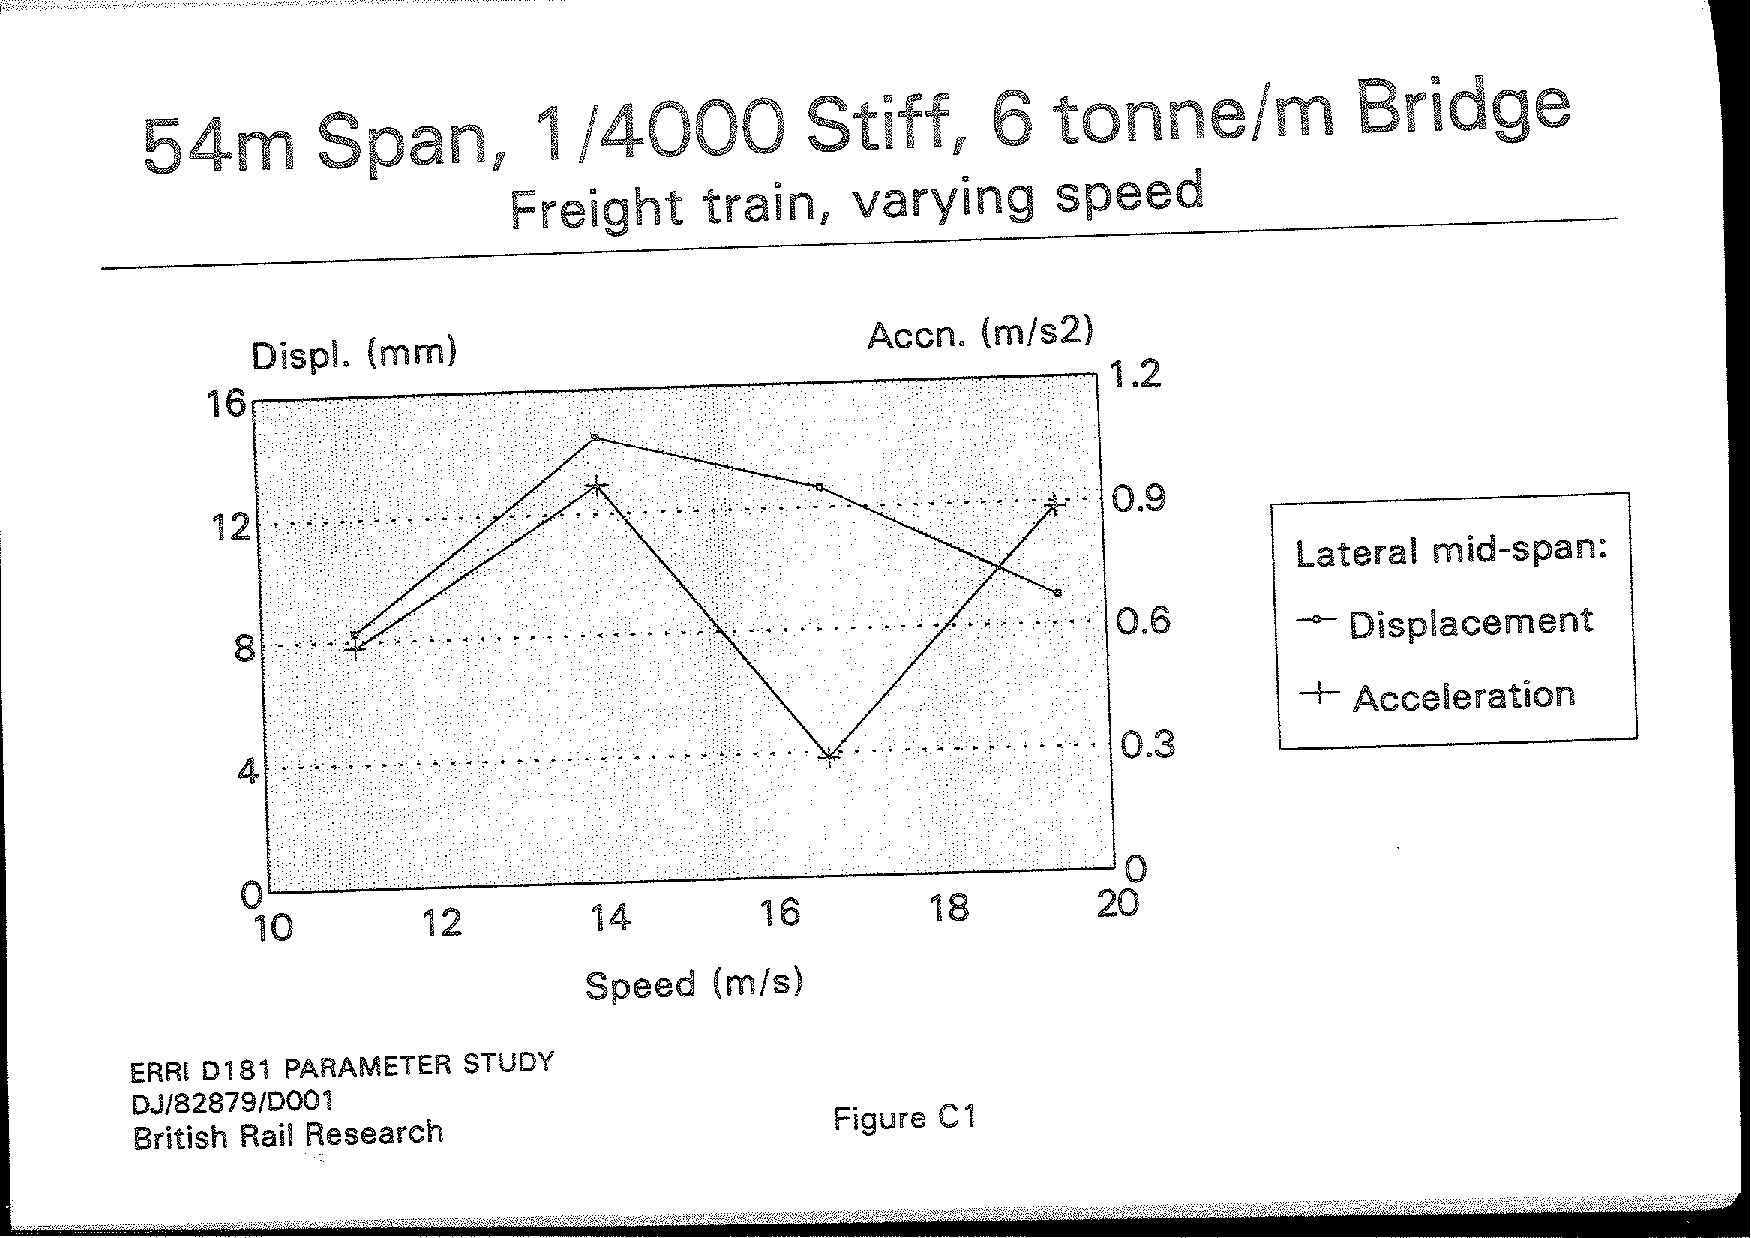
\includegraphics[width=0.8\textwidth]{c1}
    \caption{Figure C1 extracted from \citet{d181dt329} }
    \label{fig:c1}
\end{figure}

\begin{figure}[h!]
    \centering
    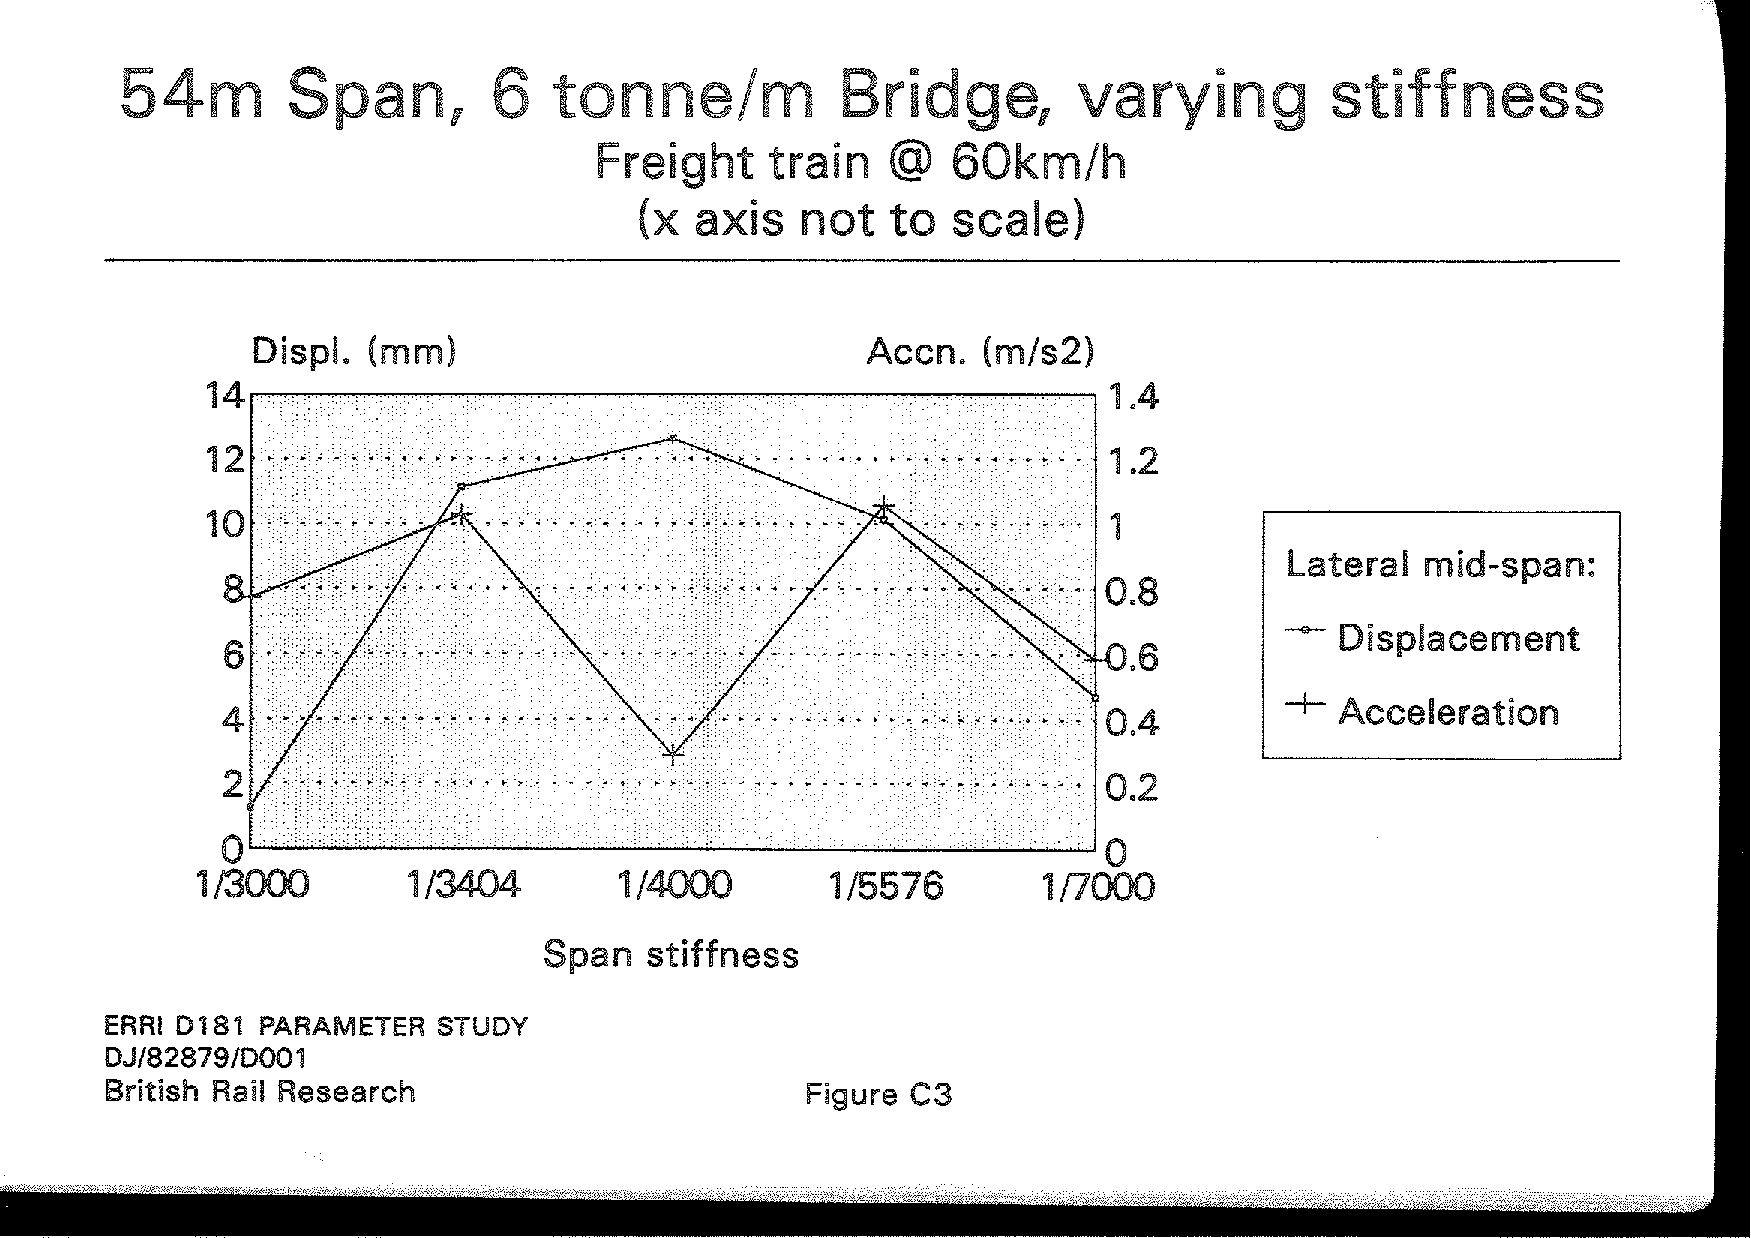
\includegraphics[width=0.8\textwidth]{c3}
    \caption{Figure C3 extracted from \citet{d181dt329} }
    \label{fig:c3}
\end{figure}

\begin{figure}[h!]
    \centering
    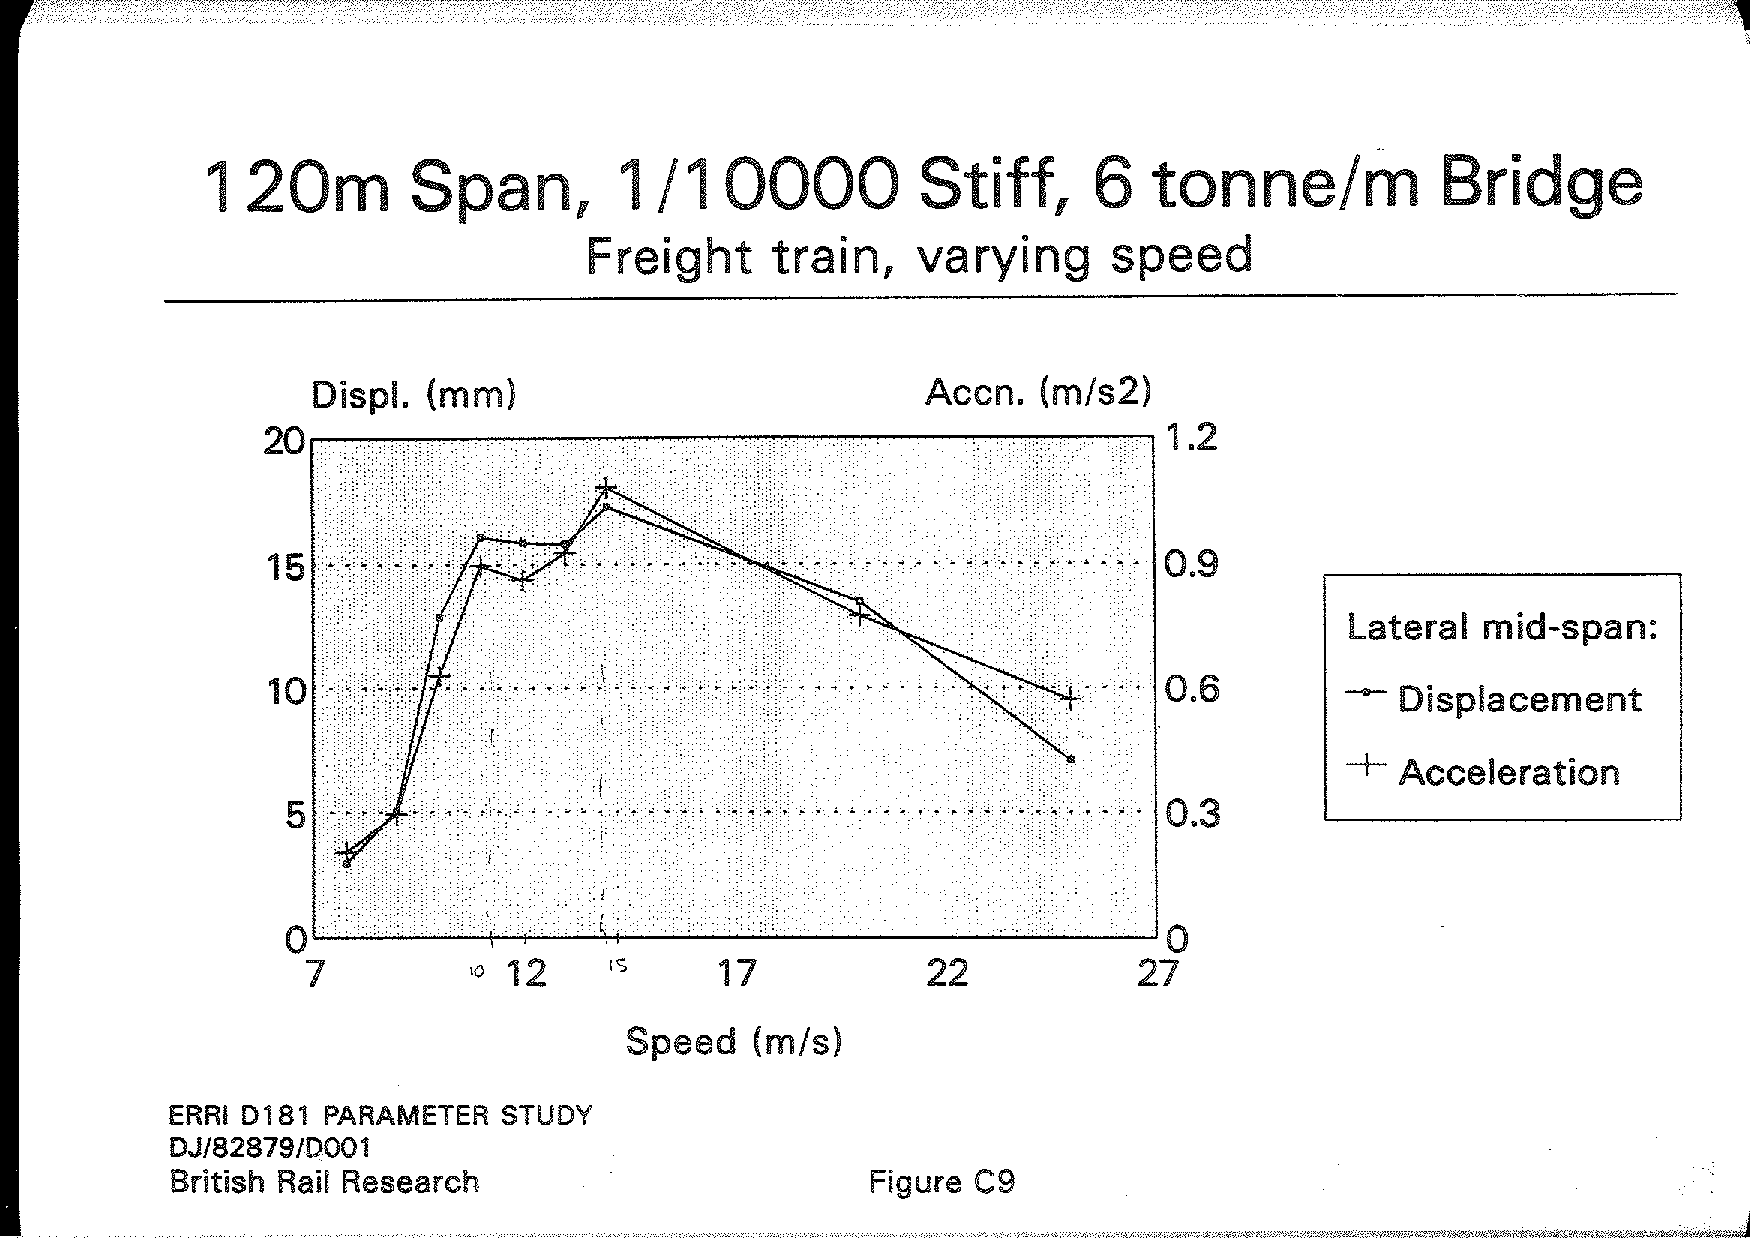
\includegraphics[width=0.8\textwidth]{c9}
    \caption{Figure C9 extracted from \citet{d181dt329} }
    \label{fig:c9}
\end{figure}

By observing Eq.\ref{eq:v(x,t)simpleharmonic}, it is concluded that force amplitude is an independent variable and perfectly linear to the analytical output. Thus the equivalent force is obtained by inputing bridge parameters and train speed into the analytical solution Eq.\ref{eq:v(x,t)simpleharmonic} and manually increasing the force amplitude little by little until the peak response output reaches the same magnitude of peak simulation output. The parameters used and their corresponding results are presented in Table.\ref{tab:parametersetupsandequivalentforce}.


\begin{table}[h!]
    \centering
    \caption{Parameter setups and equivalent force amplitude for C1,C3,C9}
    \begin{tabular}{c|ccc}
        \hline
        & C1 & C3 & C9 \\
        \hline
        Stiffness($\sfrac{\delta_0}{l}$) & 1/4000 & 1/4000 & 1/10000 \\
        Span($m$) & 54m & 54 & 120 \\ 
        Mass per unit length($kg/m$) & 6000 & 6000 & 6000\\
        Speed of train($m/s$) & 14 & 16.67(60km/h) & 14\\
        Damping ratio & 1\% & 1\% & 1\%\\
        Train type & Freight & Freight & Freight \\
        Track & Coupled freight track & Coupled freight track & Coupled freight track \\
        \hline
        Equivalent load amplitude(kN) & 14 & 15 & 14 \\
        \hline
    \end{tabular}
    \label{tab:parametersetupsandequivalentforce}
\end{table}

\subsection{Key parameter for equivalent force amplitude and hypothesis expression for refined load model}\label{sec:keyparameterforequivalentamplitudeandhypothesis}

By observing the equivalent load amplitude illustrated in Table.\ref{tab:parametersetupsandequivalentforce}, it is found that the equivalent load amplitude yielded by analytical solution meets the general principle of lateral track force concluded by DT329 track quality research. The general principle is that the lateral force is only relevant to speed if track quality and wheel conicity are fixed. And lateral force is irrelevant to the bridge parameters.
 
Because equivalent force amplitude meets the general lateral force principle, it is further expected that the equivalent force amplitude also has a similar form of force-speed relationship of DT329 VAMPIRE simulations. Due to the lack of reference data, it is impossible to make a reliable regression. Only a hypothesis expression can be created by scaling Eq.\ref{for:regressionfreight} to 14kN at 14m/s(reference data set C1). Please note only C1 was used in creating the hypothesis expression so C3 and C9 remains available for the verification.

\begin{equation}
    Q= 1928\times c^{0.7495}
\end{equation}

where:

$Q$: equivalent force amplitude($N$)

$c$: speed of the train($m/s$)

This scaling is reasonable because: according to the conclusion of DT329 track quality research, lateral forces generated on 7mm standard deviation tracks has a certain relationship with speed(Eq.\ref{for:regressionfreight}). And it is also concluded that at same speed, lateral forces are linear to the track stand deviation. Thus, since all 3 reference data are run on the same track, force output of analytical model at each speed(14m/s and 16.67m/s) could be scaled from Eq.\ref{for:regressionfreight} 's results at these speeds. Furthermore, a scale factor is then applied on Eq.\ref{for:regressionfreight} to reflect the scaling to the whole speed domain and this yields above equation.

As a conclusion, this hypothesis expression is obtained by processing the output of VAMPIRE simulation on freight trains and coupled freight track(poorer than passenger line and high speed line). So it is in closest prediction in the effects generated by freight trains. However, since passenger trains and high speed trains yields lower lateral force compared with freight trains, this hypothesis expression remains conservative for all train types.

\section{Verification of the method}

In this section the combined usage of analytical model and hypothesis expression for equivalent force amplitude is examined and verified. A matlab script is written to function the analytical model with hypothesis expression for equivalent load amplitude implemented. Now that force amplitude $Q$ is a function of speed, it's no longer necessary to input the force amplitude manually. To verify the correctness of combined usage of these two elements, other reference data from resonance research in DT329 are selected and presented in Figure.\ref{fig:c12}, \ref{fig:c13} and \ref{fig:c14}. 

\begin{figure}[h!]
    \centering
    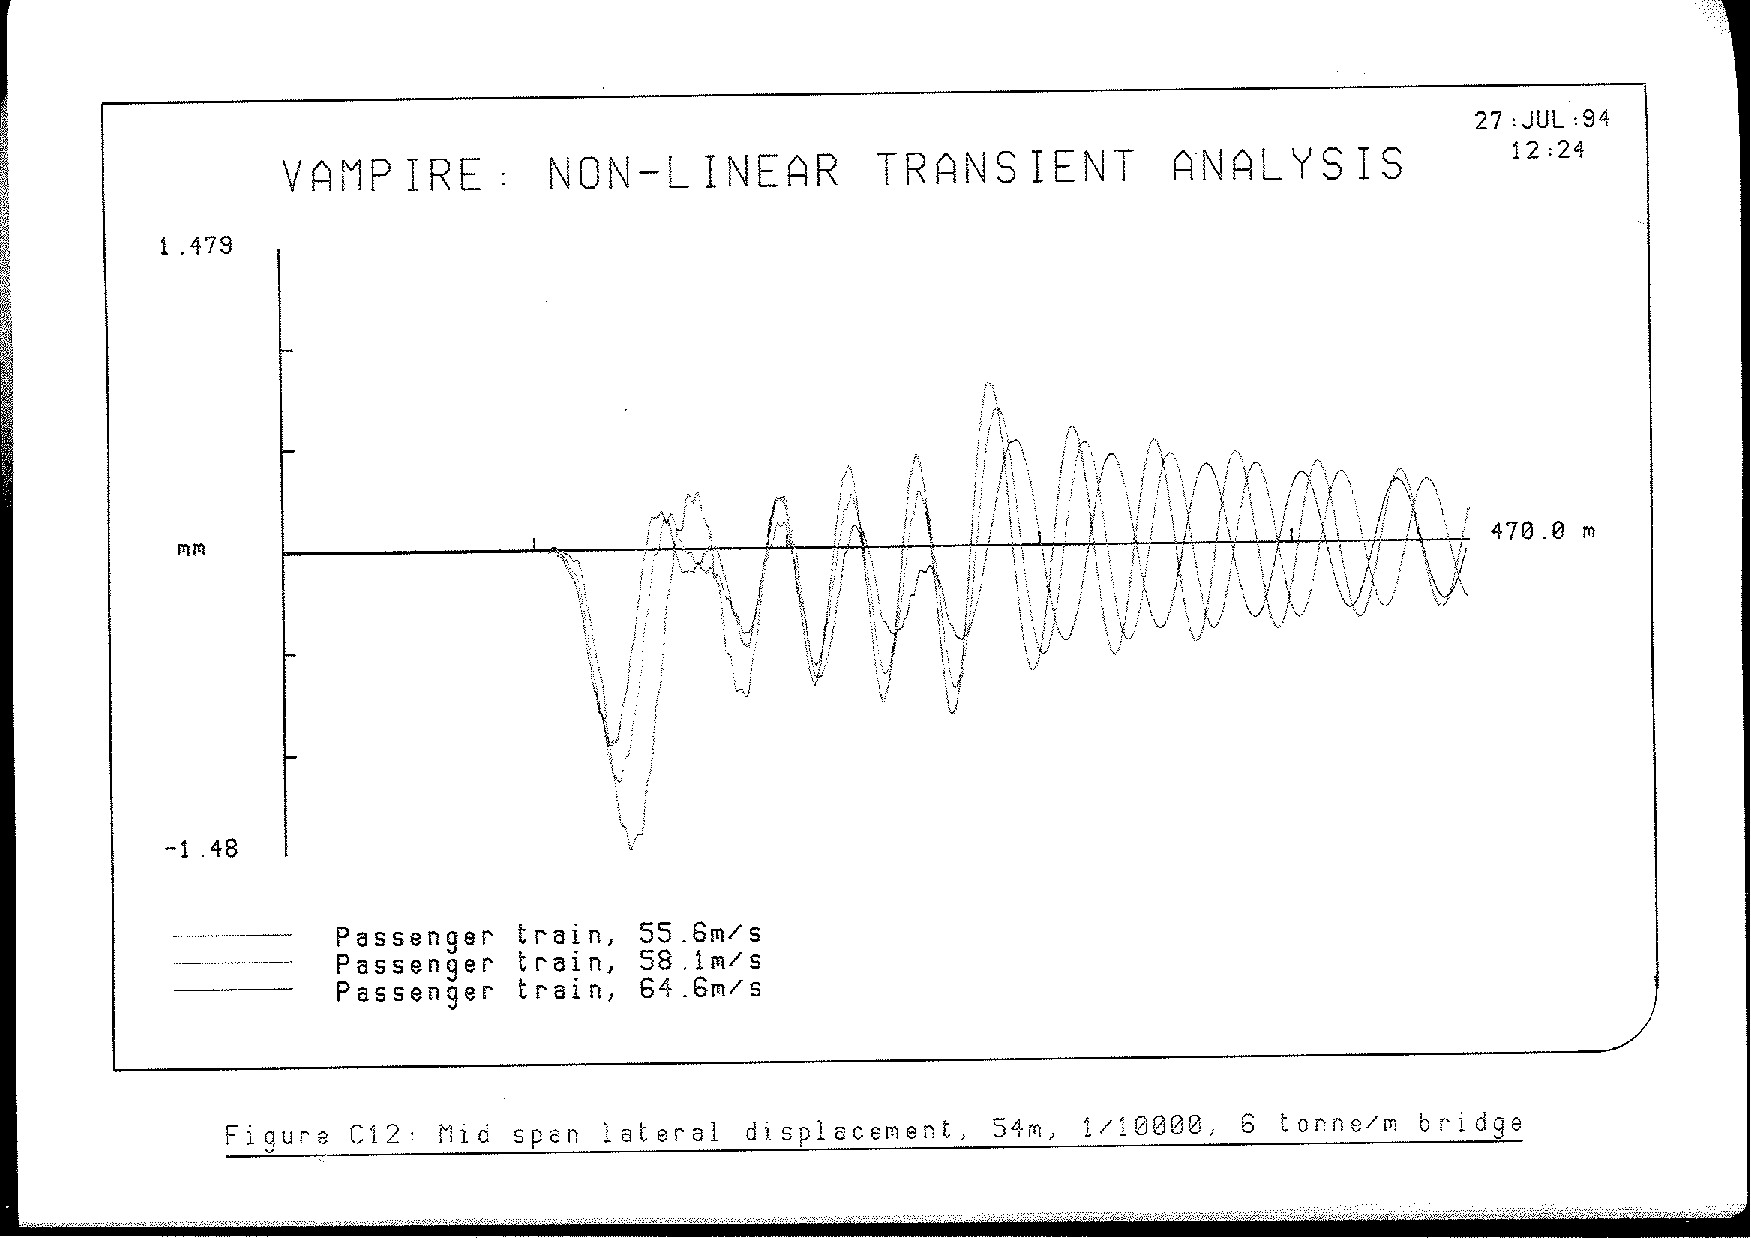
\includegraphics[width=0.8\textwidth]{c12}
    \caption{Figure C12 extracted from \citet{d181dt329} }
    \label{fig:c12}
\end{figure}

\begin{figure}[h!]
    \centering
    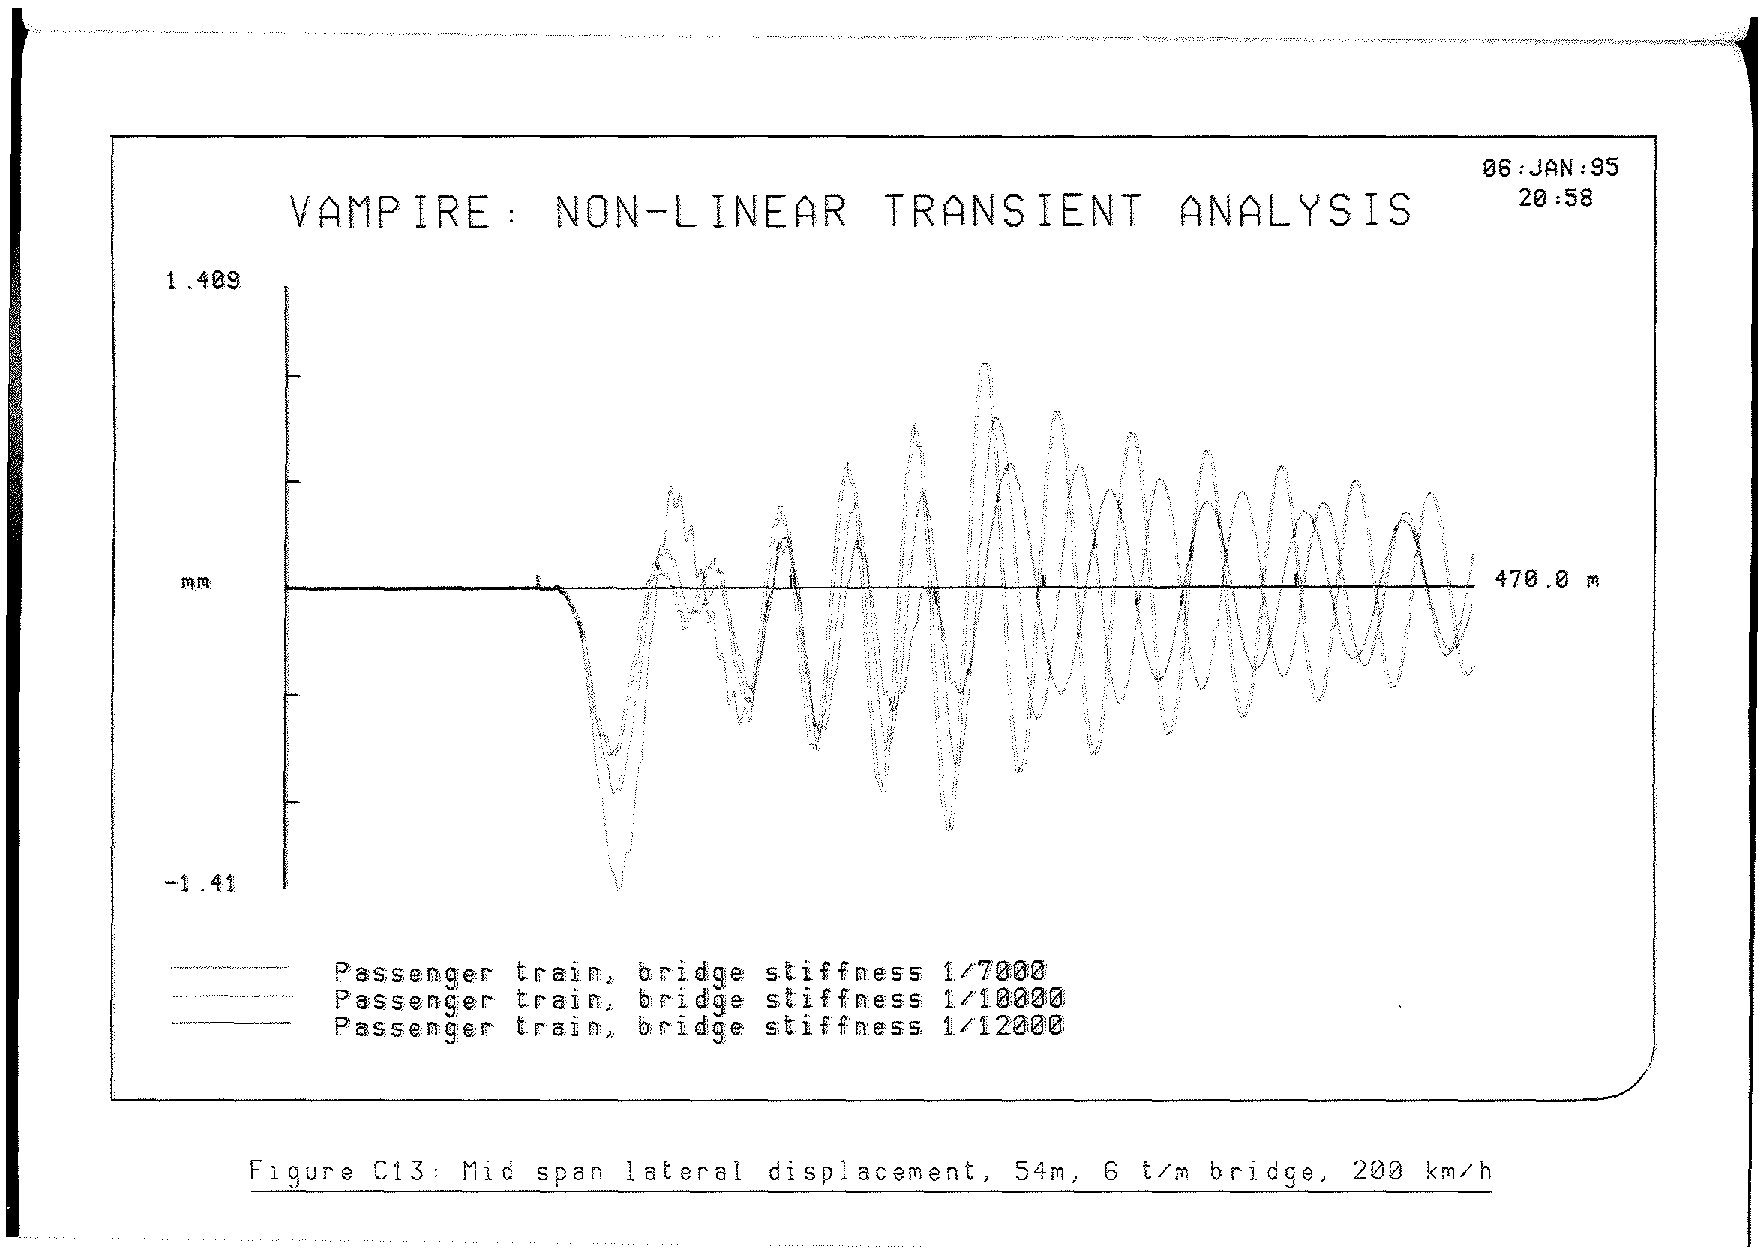
\includegraphics[width=0.8\textwidth]{c13}
    \caption{Figure C13 extracted from \citet{d181dt329} }
    \label{fig:c13}
\end{figure}

\begin{figure}[h!]
    \centering
    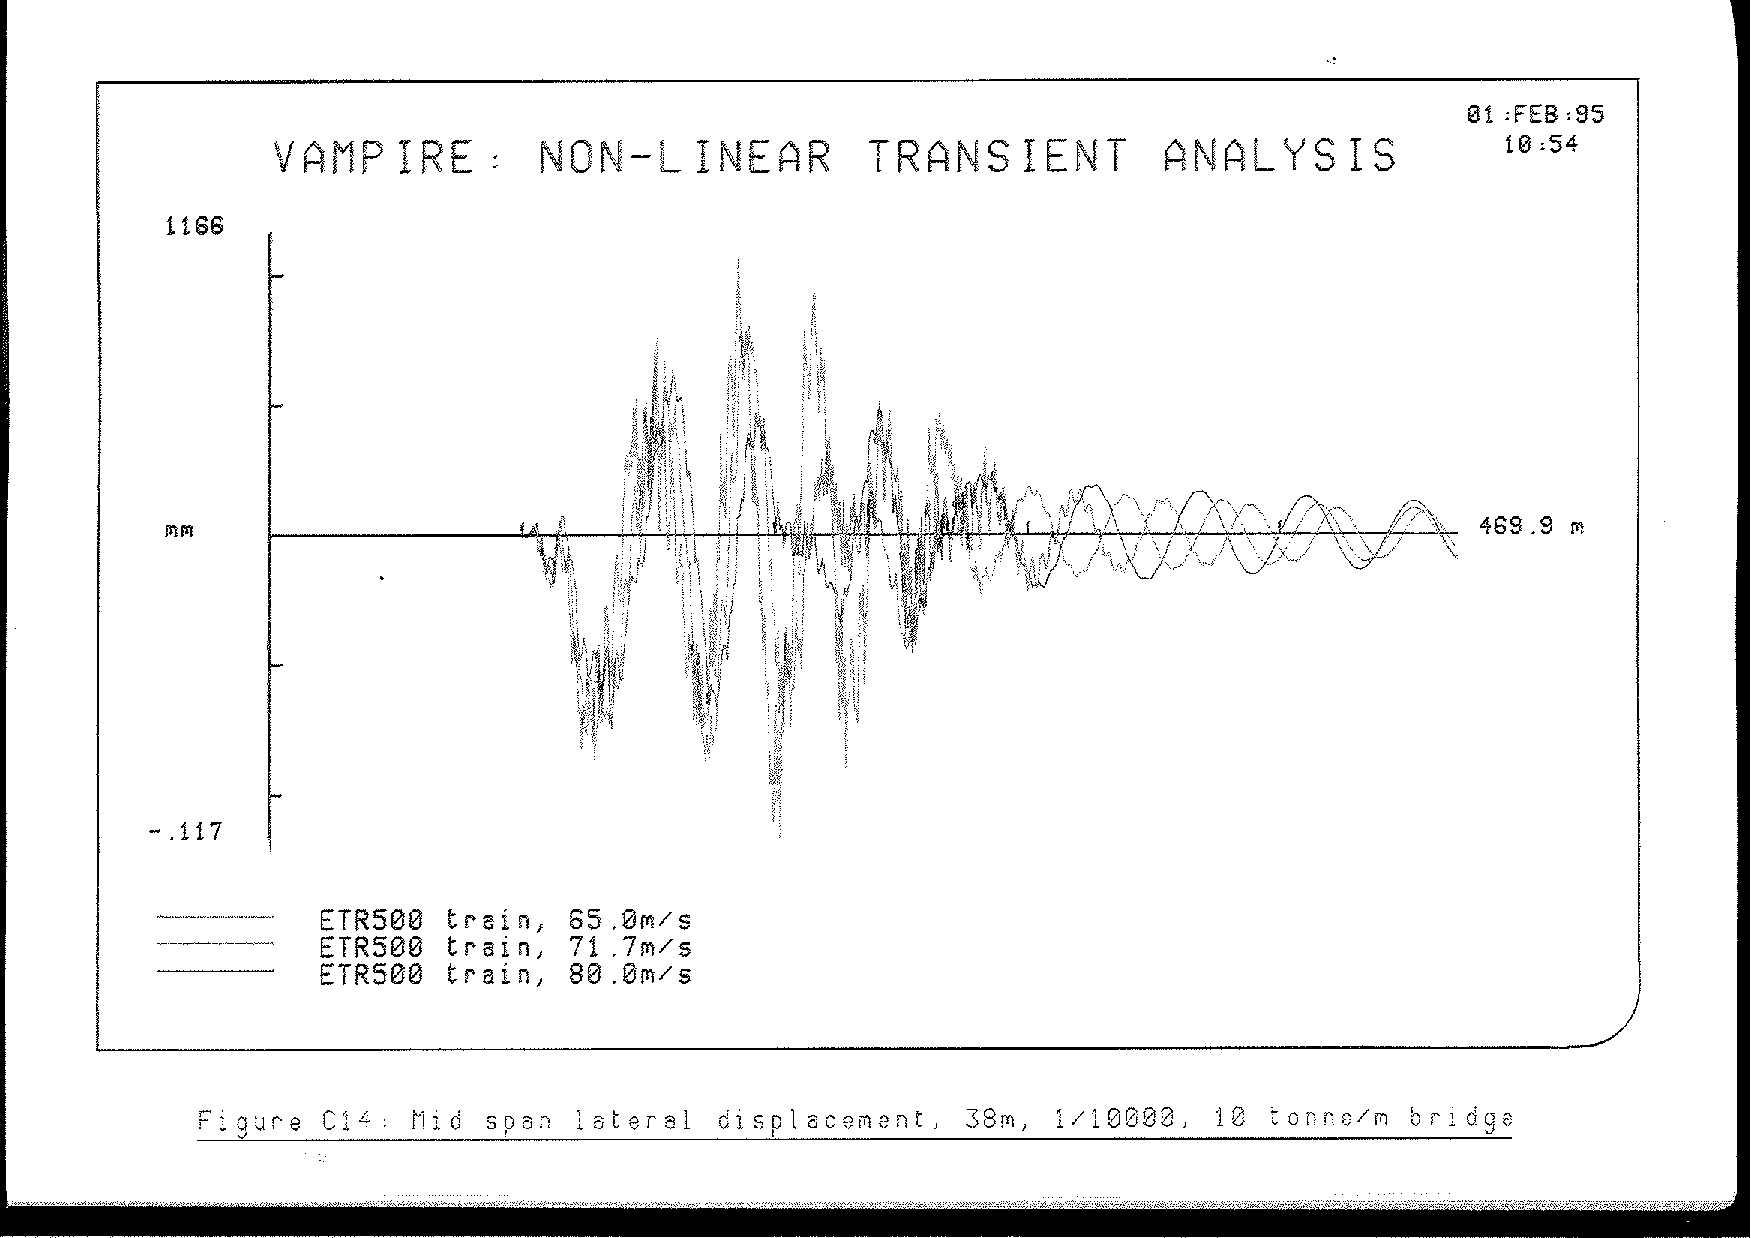
\includegraphics[width=0.8\textwidth]{c14}
    \caption{Figure C14 extracted from \citet{d181dt329}. An minor error is observed in y-axis label. Upper boundary of y-axis should be 0.116 }
    \label{fig:c14}
\end{figure}

To assure conservative comparison, only axle repeat pattern resonance results are selected because their output are more pronounced than kinematic resonance effect. Altogether 5 sets of reference data are selected. They include 2 reference data for freight trains(C3,C9), 2 reference data for passenger train(C12,C13) and 1 reference data for high-speed train(C14). Due to the fact that freight trains yield greater force than the other two types of trains, the analytical result should be conservative for the latter 3 cases. Since the output of C3 and C9 are already presented in Table.\ref{tab:parametersetupsandequivalentforce} so they are not being presented with other 3 sets of data this time. The bridge parameters and trains speed involved in these 3 cases(C12,C13,C14) are input into the analytical solution to yield analytical results.

\begin{table}[h!]
    \centering
    \caption{Comparison of results of simulation output and analytical output using refined load model}
    \begin{tabular}{c|ccc}
        \hline
         & C12 & C13 & C14\\
        \hline
        Stiffness($\sfrac{\delta_0}{t}$) & 1/10000 & 1/12000 & 1/10000\\
        Span($m$) & 54 & 54 & 38\\
        Mass per unit length($kg/m$) & 6000 & 6000 & 10000\\
        Speed of train($m/s$) & 55.6 & 55.6 & 65\\
        Damping ratio & 1\% & 1\% & 1\%\\
        Train type & Passenger & Passenger & High speed \\
        Track & Passenger Track & Passenger Track & High speed track\\
        \hline
        Peak Simulation displacement($mm$) & 1.48 & 1.41 & 0.117\\
        Peak Analytical displacement($mm$) & 6.6 & 5.8 & 3.0 \\
        \hline
    \end{tabular}
    \label{tab:comparisonresultssimulationanalytical}
\end{table}


In Table.\ref{tab:comparisonresultssimulationanalytical} the parameters involved in these 3 cases and their corresponding peak analytical results as well as peak simulation results are presented. 



\begin{figure}[h!]
\centering
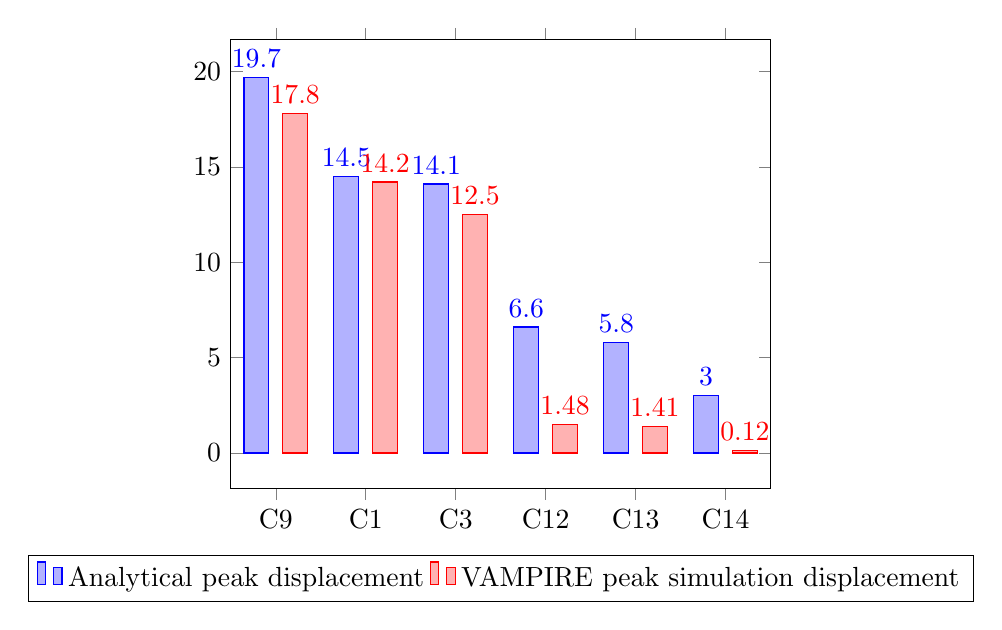
\begin{tikzpicture}
\begin{axis}[
    symbolic x coords={C9,C1,C3,C12,C13,C14},
    xtick=data,
    legend style={at={(0.5,-0.15)},
        anchor=north,legend columns=-1},
    ybar=5pt,% configures `bar shift'
    bar width=9pt,
    nodes near coords,
]
\addplot 
    coordinates {(C9, 19.7) (C1, 14.5) (C3, 14.1)   (C12,6.6) (C13,5.8) 
        (C14, 3.0) };
\addplot 
    coordinates {(C9, 17.8) (C1, 14.2) (C3, 12.5)  (C12,1.48) (C13,1.41)
         (C14,0.117) };
\legend{Analytical peak displacement,VAMPIRE peak simulation displacement}
\end{axis}
\end{tikzpicture}
\caption{Comparison between VAMPIRE peak simulation result and analytical peak result}
\label{fig:comparisonpeaksimulationanalytical}
\end{figure}

To clearer illustrate the comparison of both peak results from simulation and analytical, Figure.\ref{fig:comparisonpeaksimulationanalytical} is created with rearranged x-axis order to make the descending trend more obvious. Please note all data sets except for C1 are valid for verification(C1 is used in creation of expression).

It can be seen that analytical results always keep a conservative margin above the simulation results. As expected, margins for C12,C13,C14 are bigger compared to C9,C1,C3 proofs that the analytical solution becomes more conservative if adopted to passenger train and high-speed train. What's more, the descending trend of analytical results follows the descending trend of simulation results perfectly regardless of train types. Thus considering these reasons, the analytical solution is sufficient for universal application on all train types.

\chapter{Finalizing the method for practical usage using real bridge parameters}

In practical usage, the speed that generates the highest peak response is unknown. Thus it is necessary to obtain the peak response for all speeds within the possible speed range. This is done by iterating the existing Matlab script with different speed. The increment in speed iteration is set in a way that ensures at least 1000 runs are done to guarantee precession. An example is illustrated as follows to show the usage on a real bridge project.

For an arch railway bridge located near Amsterdam, first step to is to collect following parameters:

$L = 255m$, $m = 5222e3kg$, $\mu = 2.0478e4 kg/m$, $EJ = 6.56e12Nm^2$

where:

$L$: span of the bridge

$\mu$: uniform mass per unit length of the bridge

$EJ$: lateral stiffness of the bridge

to test through a speed range of $1m/s - 30m/s$

Before beginning the calculation, make sure you have fog.m and Speedenvelop.m in your current working directory. By inputting following command in Matlab console, 

\texttt{Speedenvelop(6.56e12,255,2.0478e4,1,30,0.01)}


the envelop for displacement is generated and illustrated in Figure.\ref{fig:spedefEJ6560000000000L255min1max30mu20478.tikz}

\begin{figure}[h!]
\centering 
\setlength\figureheight{6cm} 
\setlength\figurewidth{6cm} 
% This file was created by matlab2tikz v0.4.7 (commit 29117077607177efe915cc01d961cced006239c8) running on MATLAB 8.3.
% Copyright (c) 2008--2014, Nico Schlmer <nico.schloemer@gmail.com>
% All rights reserved.
% Minimal pgfplots version: 1.3
% 
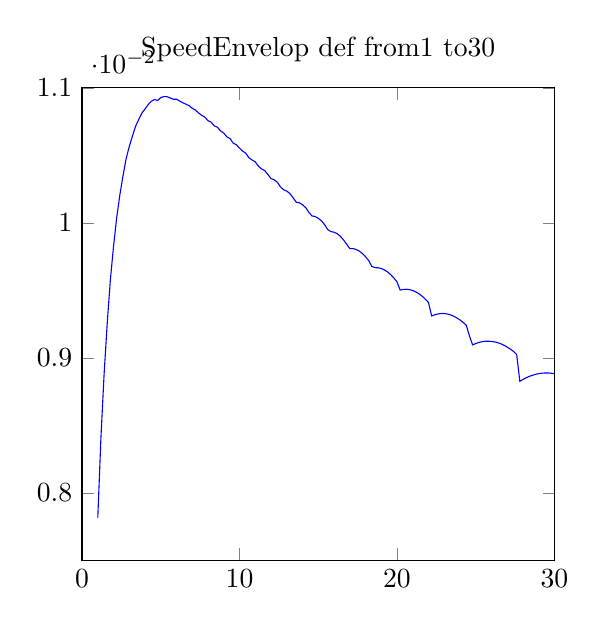
\begin{tikzpicture}

\begin{axis}[%
width=\figurewidth,
height=\figureheight,
scale only axis,
xmin=0,
xmax=30,
ymin=0.0075,
ymax=0.011,
title={SpeedEnvelop def from1 to30}
]
\addplot [color=blue,solid,forget plot]
  table[row sep=crcr]{%
1	0.00781568842060085\\
1.2	0.00840892567977264\\
1.4	0.0088768875903958\\
1.6	0.00925769529057003\\
1.8	0.00957910144655464\\
2	0.00982648840148397\\
2.2	0.0100372557099215\\
2.4	0.0102060089657038\\
2.6	0.010347841028453\\
2.8	0.0104753362289414\\
3	0.010566090236029\\
3.2	0.0106426943938749\\
3.4	0.0107156879259678\\
3.6	0.0107656368912521\\
3.8	0.0108134770961416\\
4	0.0108433829006734\\
4.2	0.0108762461970553\\
4.4	0.0109009754438711\\
4.6	0.0109137058875431\\
4.8	0.0109063964703489\\
5	0.0109283926778865\\
5.2	0.0109354115709882\\
5.4	0.010934364378216\\
5.6	0.010925358882146\\
5.8	0.0109155184260617\\
6	0.0109160952245694\\
6.2	0.0109022893020932\\
6.4	0.0108894990281659\\
6.6	0.0108791296950589\\
6.8	0.0108683159097076\\
7	0.0108485530748728\\
7.2	0.0108354499334163\\
7.4	0.0108143121429067\\
7.6	0.0107967054438007\\
7.8	0.0107826189027167\\
8	0.0107571129205081\\
8.2	0.0107450192698353\\
8.4	0.0107182431373167\\
8.6	0.0107081009100856\\
8.8	0.0106810097968274\\
9	0.0106647893596357\\
9.2	0.0106368269751327\\
9.4	0.0106244435627288\\
9.6	0.0105902161380316\\
9.8	0.0105787489298167\\
10	0.0105530497685275\\
10.2	0.0105311301588914\\
10.4	0.0105155111529359\\
10.6	0.0104818416711415\\
10.8	0.0104658192794055\\
11	0.0104515232844051\\
11.2	0.0104195968460413\\
11.4	0.0103992383576141\\
11.6	0.0103875827376142\\
11.8	0.0103585518798102\\
12	0.0103282987036047\\
12.2	0.0103183620397562\\
12.4	0.0103012474040927\\
12.6	0.0102668977746374\\
12.8	0.0102449204320541\\
13	0.0102354809790005\\
13.2	0.0102169579397151\\
13.4	0.0101865143682396\\
13.6	0.0101530378665145\\
13.8	0.0101488592884028\\
14	0.0101342026283539\\
14.2	0.0101129828210581\\
14.4	0.0100781640001081\\
14.6	0.010051230942275\\
14.8	0.0100463931273211\\
15	0.0100339102223161\\
15.2	0.0100154789040376\\
15.4	0.00998674150551577\\
15.6	0.00995047989615967\\
15.8	0.00993544019804088\\
16	0.00993088834100722\\
16.2	0.0099199018939231\\
16.4	0.00990104705345698\\
16.6	0.00987441551082942\\
16.8	0.00984237739719204\\
17	0.00980928040956712\\
17.2	0.0098093242438416\\
17.4	0.00980329783311577\\
17.6	0.00979122702961792\\
17.8	0.00977314390458511\\
18	0.00974908670711774\\
18.2	0.00972108217302529\\
18.4	0.0096776691907686\\
18.6	0.00966812567615805\\
18.8	0.0096672743699076\\
19	0.00966167442250244\\
19.2	0.00965133478148734\\
19.4	0.00963626874305325\\
19.6	0.00961649393213872\\
19.8	0.00959203227865456\\
20	0.00956290998985286\\
20.2	0.0095021185042862\\
20.4	0.00950695108828918\\
20.6	0.00950797086177456\\
20.8	0.00950518266938973\\
21	0.00949859410737403\\
21.2	0.00948821551471712\\
21.4	0.00947405996230233\\
21.6	0.00945635016311157\\
21.8	0.00943490732597904\\
22	0.00940971735699768\\
22.2	0.00931048059107463\\
22.4	0.00931929357671497\\
22.6	0.00932536783564737\\
22.8	0.00932827887006457\\
23	0.00932803971339443\\
23.2	0.00932466491318731\\
23.4	0.00931817052503146\\
23.6	0.00930857410555171\\
23.8	0.00929589470449585\\
24	0.0092803683442182\\
24.2	0.00926243390849551\\
24.4	0.0092414380792758\\
24.6	0.00916278336234724\\
24.8	0.00909609061802426\\
25	0.00910564521095271\\
25.2	0.00911382028447303\\
25.4	0.00911959836984988\\
25.6	0.00912274595493189\\
25.8	0.00912328389307619\\
26	0.00912136767440461\\
26.2	0.00911807810466714\\
26.4	0.00911219402539695\\
26.6	0.00910373969614448\\
26.8	0.0090927400294876\\
27	0.00907945686157787\\
27.2	0.00906461860626204\\
27.4	0.00904726523290454\\
27.6	0.00902380873477224\\
27.8	0.00882644457839617\\
28	0.00883996385182427\\
28.2	0.00885231633946435\\
28.4	0.00886244919403873\\
28.6	0.00887051931610704\\
28.8	0.00887784576510649\\
29	0.0088829756466977\\
29.2	0.00888593368675971\\
29.4	0.00888785865101469\\
29.6	0.00888798738354364\\
29.8	0.00888597303168551\\
30	0.00888235391855735\\
};
\end{axis}
\end{tikzpicture}% 
\caption{Peak deflection at mid-span with regard to changing train speed. Parameters: $EJ = 6.56e12Nm^2$, $L= 255m$,$\mu = 20478 kg/m$, $c_{min}=1m/s$, $c_{max} = 30m/s$} 
\label{fig:spedefEJ6560000000000L255min1max30mu20478.tikz} 
\end{figure}

The plot shows that the critical speed appears at approximately $5m/s$ and corresponding peak deflection response is approximately $11mm$. 

Since the relationship between end support rotation angle and mid-span deflection is widely known as:

$$ \varphi = \frac{3}{L}\cdot \delta_0  $$

and rotation is yielded as:

$$ \varphi = \frac{3}{255}\times 0.011 = 0.00013 $$

This value is much lower than the rotation value regulated in EN1991-2. See Section.\ref{sec:Transverse-deformations-and-vibrations} for criteria details.

Thus the conclusion can be made that this bridge is safe subjected to lateral dynamic load.

However, if encountering unfavourable peak result, a filter can be applied on the train speed to further cut off the peak response. In previous chapter it has been already be concluded that all resonance effects between train and bridge are wavelength phenomenon. In order to couple frequency with bridge's first natural bending frequency, the train needs to operate at a certain speed range. 

For example, according to Chapter.\ref{sec:wavelengthstudy}, the possible wavelength range for trains in the Netherlands is approximately 10m-30m, including both axle repeat wavelength and kinematic wavelength. 

The natural frequency of the bridge in this example is 

$$ f_1 = \frac{\pi}{2l^2}\sqrt{\frac{EJ}{\mu}} = \frac{\pi}{2\times 255^2}\sqrt{\frac{6.56e12}{1.0478e4}} = 0.4Hz$$

so the possible resonance speedis obtained by multiplying wavelength range with natural frequency, yielding: $4m/s$ and $12m/s$

Although this speed filtering range doesn't help to cut off maximum response in this case because critical speed stills remains in the speed range, the filter can be more effective for bridges possessing higher first natural frequency simply because both lower and upper boundary for speed filtering range is linear to beam's first natural frequency. While it's not likely for upper boundary to shift to the left side of the critical speed, it's more favourable for lower boundary to shift to the right side of the critical speed.

\section{Conclusion}

The new practical method for checking lateral resonance response of railway bridge is developed in this chapter. This method is capable to simulate a resonance scenario where the bridge was passed by a moving railway vehicle. 

The method shows conservative prediction compared to VAMPIRE simulations. However, since lack of data can be used to further verify the practical method, results on longer span bridges can not be verified until new simulations or measurements data are obtained.

A general conclusion in finalizing phase of practical method is, for a certain bridge, faster train speed doesn't necessary cause higher resonance response of the bridge. As can be seen in Figure.\ref{fig:spedefEJ6560000000000L255min1max30mu20478.tikz}, critical speed appears at approximately $5m/s$, and response start to fall when speed is higher than $5m/s$. This means comparing to higher load amplitude caused by higher train speed, the shorter loading time caused by same reason is more dominating. By considering the fact in Figure.\ref{fig:comparisonpeaksimulationanalytical} that the analytical is even more conservative for higher speed, it can be concluded than high-speed trains cause less dynamic problem for lateral bridge dynamics.

Matlab scripts are already written and attached for the convenience of readers. Since the explicit solution has been given in the chapter, it's completely possible to adopt them in other mathematical software for different preferences.


\chapter{Recommendations on improvement on Eurocode}


\section{Recommandations of this thesis}

It is advised that Eurocode committee spend more effort in providing background information to structural designers on cross-field topics. For example, railway bridge engineering is related to both fields of structural engineering and railway engineering. The knowledge of railway engineering is seldomly known among structrual engineers and they hardly know the key to the problem. So it is vital for the code to provide its users with sufficient background information.

This can be done by adding references of various statements and criteria. Even with good luck, this thesis spent over 3 month of time in trying to find the original research documents for the 1.2Hz criterion. And it can be expected that if no reference is recorded, finding the source would be even more difficult for other researches in the future.

By simply adding reference to the criteria, this amount of wasted time could be saved for a better course. Thus this thesis suggest references to be added for the sake of future researches/designs.

Also, this thesis suggests make deeper evaluation on the criteria being adopted in the code. At least in this report it is found that the 1.2Hz criterion isn't a correct verification strategy. 

Last but not least, this thesis suggests Eucocode committee possess a further vision for the future. For example, in EN1991-2 railway bridge dynamics, there's no instruction can be found for bridges with span longer than 150m in the logic diagram. This means during the creation process of EN1991-2, the possibility of longer span bridges in the future is neglected, causing potential problem for future designs. 

\section{Other lateral railway bridge dynamics related criteria extracted from other codes}
Following sections provides several orientations for improving criteria for lateral bridge dynamics in terms of safety and serviceability of running stock.


\subsection{Requirements for traffic safety(horizontal)}
Requirements other than bridge first lateral frequency higher than 1.2Hz. Since there's no further requirements mentioned by Eurocode, following requirements are gathered from other European codes, eg. British standards, UIC leaflet, etc.

\begin{enumerate}[-]
    \item Requirements regarding traffic safety for vehicles
    \begin{enumerate}
        \item Guiding Force: \citet{code2005518} , \citet{en200714363} and\citet{cuadrado2008analysis} propose safty limitations against railway vehicle overturning. From\citet{en200714363} the maximum guiding force for a vehicle with a load per axle of 170kN(AVE) is 66kN per axle and 48kN per axle for a vehicle with a load per axle of 112kN(ICE2). For the R1 freight wagon(load per axle of 245kN), the maximum guiding force per axle is 78kN.
        \item Maximum lateral acceleration of the railway vehicle: proposed by \citet{13803}
    \end{enumerate}
    \item Requirements regarding safety for bridge\\
    \citet{EC0} A2.4.4.1(2): Horizontal transverse deflection(to ensure acceptable horizontal track radii) and horizontal rotation of a deck about a vertical axis at ends of a deck(to ensure acceptable acceptable horizontal track geometry and passenger comfort)
\end{enumerate}


\subsection{Requirements for traffic safety on derailment: Railway vehicle derailment mechanism and safety criteria}

Derailment mechanisms
\begin{enumerate}
    \item vehicle resonant response
    \item lateral instability
    \item vehicle overturning
    \item vertical wheel unloading
    \item flange climb
    \item rail roll-over
    \item track panel shift
    \item longitudinal train forces
\end{enumerate}

The four types of derailment: flange climb derailment, derailment caused by guage widening and rail roll-over, derailment caused by track panel shift, derailment cause by vehicle lateral instability have a common cause of high lateral force at the wheel-rail interface. According to \citet[Chapter 8, IV]{iwnicki2006handbook} any conditions that lead to high lateral forces or lead to lower the ability of the system to sustain the force should be corrected. 

\subsection{Flange climb derailment}
Wheel flange climb derailments are caused by wheels climbing onto the top of the railhead then further running over the rail. Wheel climb derailments generally occur in situations where the wheel experiences a high lateral force combined with circumstances where the vertical force is reduced on the flanging wheel. The high lateral force is usually induced by a large wheelset angle-of-attack. The vertical force on the flanging wheel can be reduced significantly on bogies having poor vertical wheel load equalisations, such as when negotiating rough track, large track twist, or when the car is experiencing roll resonances. 

\begin{figure}[h]
    \centering
    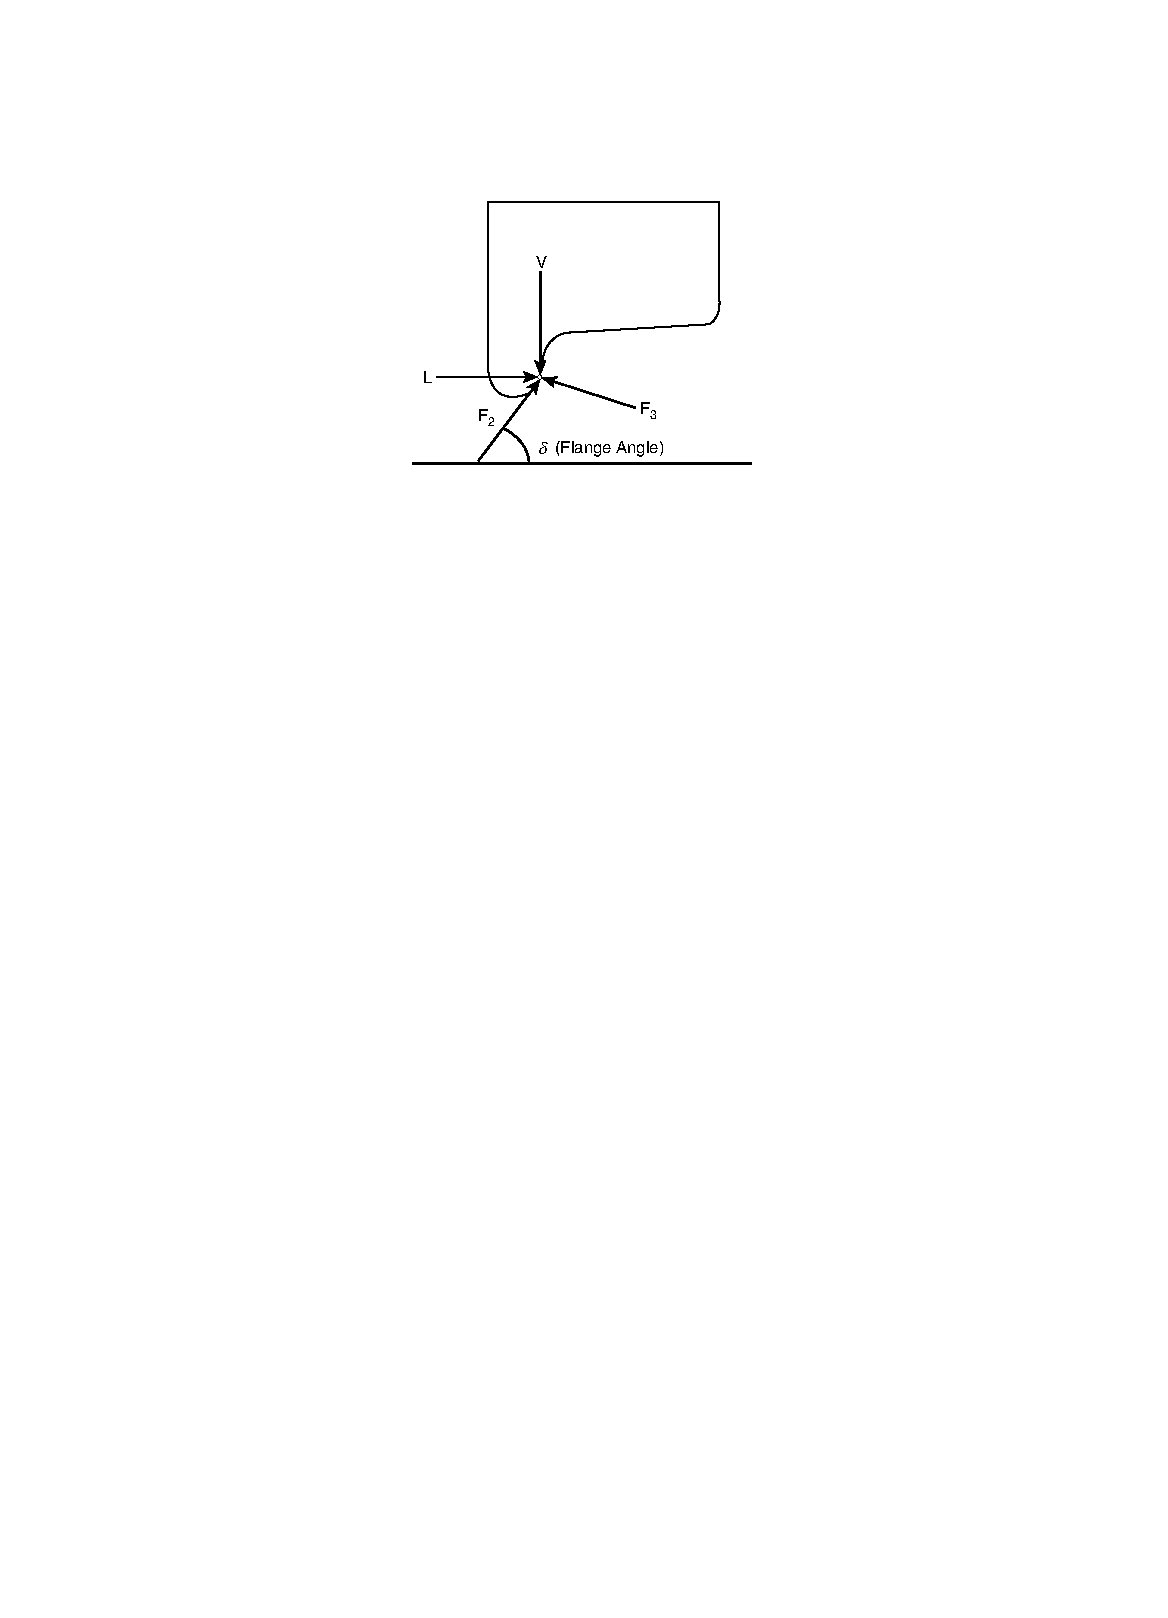
\includegraphics[width=0.4\textwidth]{forcesatflangecontactlocation.pdf}
    \caption{Forces at flange contact location. Extracted from \citet[Figure8.4]{iwnicki2006handbook}}
    \label{fig:forcesatflangecontactlocation}
\end{figure}

The criterion L/V ratio can be expressed as:

\begin{equation}
    \frac{L}{V}=\frac{\tan \delta -\frac{F_2}{F_3}}{1+\frac{F_2}{F_3}\tan \delta}
\end{equation}

Nadal's famous L/V ratio limiting criterion, given by Equation.\ref{eq:nadalcriterion}, was proposed for the saturated condition $F_2/F_3=\mu$

\begin{equation}\label{eq:nadalcriterion}
    \frac{L}{V}=\frac{\tan \delta - \mu}{1+ \mu \tan \delta}
\end{equation}

\subsection{Derailment caused by guage widening and rail rollover}
Derailments caused by guage widening usually involve a combination of wide gauges and large lateral rail defections(rail roll), as shown in Figure\ref{fig:gaugewideningderailment}. Large lateral forces from the wheels act to spread the rails in curves. Both rails may experience significant lateral translation and/or railhead roll, which often cause the nonflanging wheel to drop between rails.

\begin{figure}[h]
    \centering
    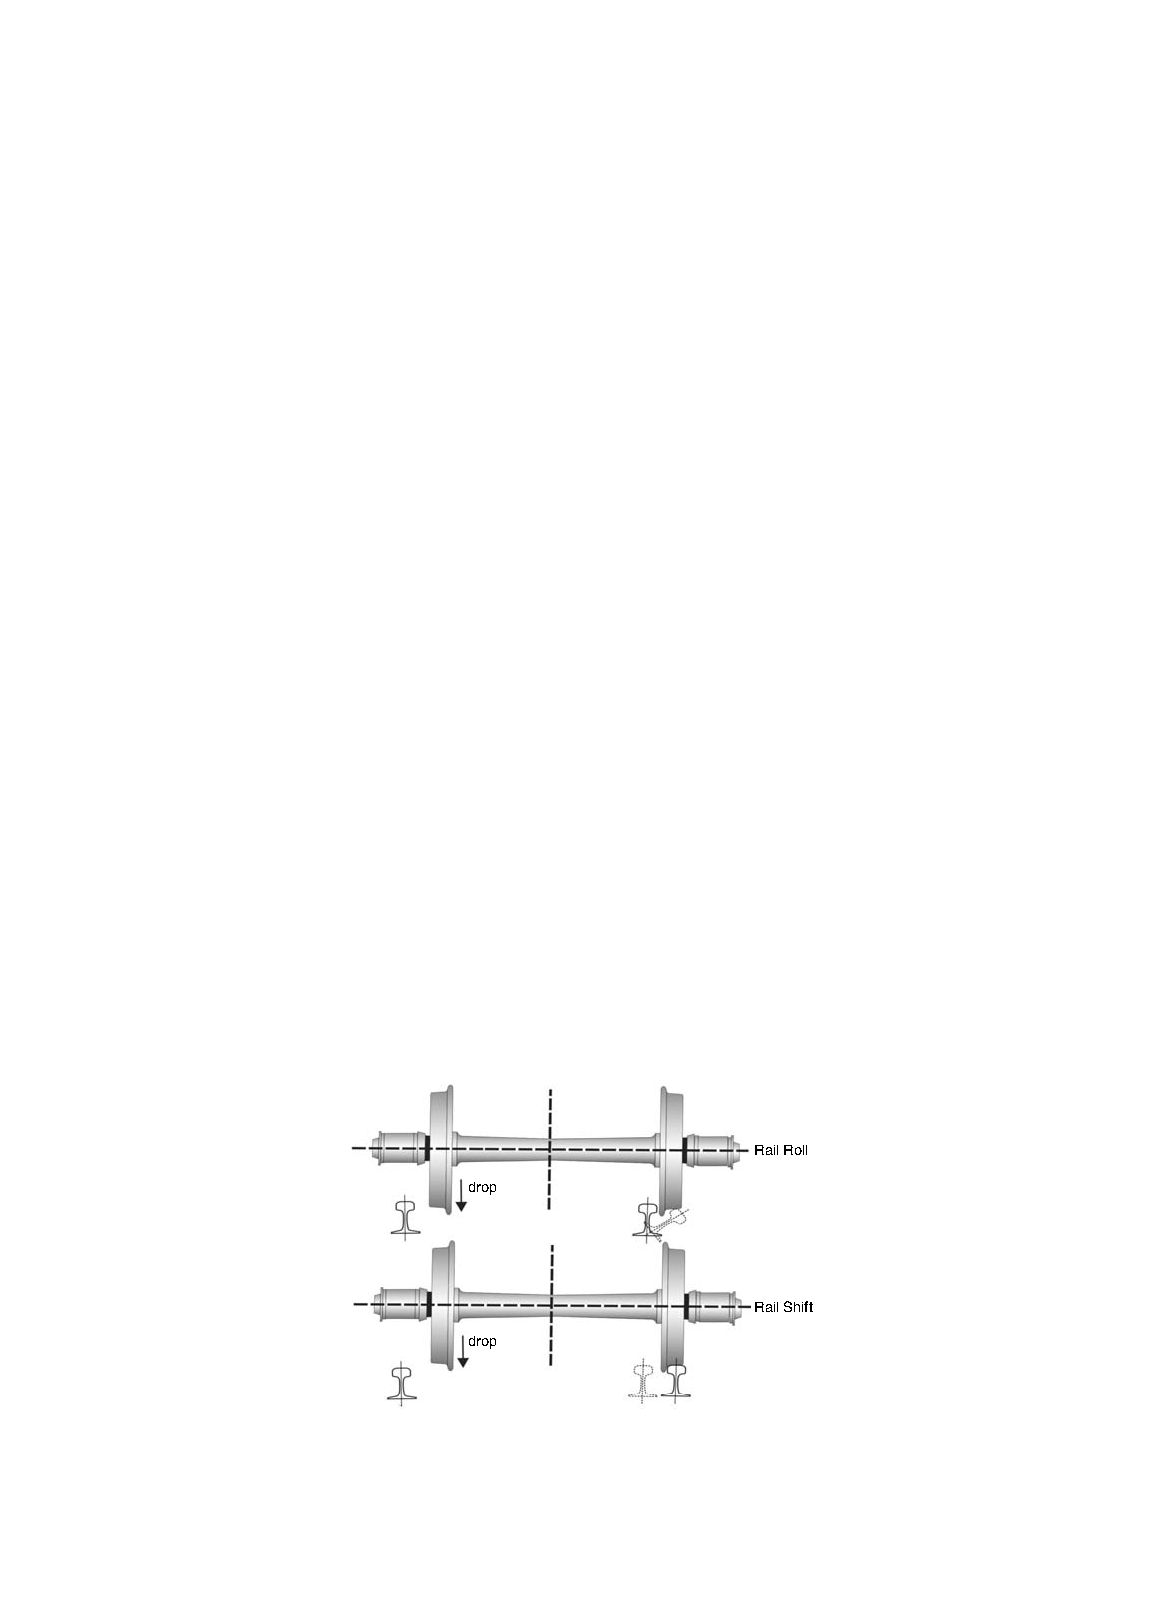
\includegraphics[width=0.8\textwidth]{gaugewideningderailment.pdf}
    \caption{Gauge widening derailment. Extracted from \citet[Figure8.18]{iwnicki2006handbook}}
    \label{fig:gaugewideningderailment}
\end{figure}

\paragraph{AAR Chapter XI rail roll criterion}
The AAR Chapter XI rail roll criterion is established by using the L/V ratio. The roll moment about the pivot point is given by,

\begin{equation}
    M=Vd-Lh
\end{equation}

under an equilibrium condition, just before the rail starts to roll, $M$ approaches to zero, then,

\begin{equation}
    \frac{L}{V}=\frac{d}{h}
\end{equation}

This L/V ratio is considered as the critical value to evaluate the risk of rail roll. When the L/V ratio is larger than the ratio of $d/h$, the risk of rail roll becomes high. The critical L/V ratio for rail roll can vary from above 0.6 for contact at the gauge side to approximately 0.2 when the contact position is at the far-field side based on the dimension of the rails. This is because the distance $d$ is reduced. Note that this L/V ratio is calculate assuming that neither the rail fasteners nor the torsional stiffness of the rail section provide any restraint.

\subsection{Derailment caused by track panel shift}
Track panel shift is the cumulative lateral displacement of the track panel, including rails, tie plates and ties, over the ballast, as shown in Figure\ref{fig:lateraltrackpanelshift}. A small shift of these components may not immediately cause the loss of guidance to bogies. However, as the situation gradually depreciates to a certain level, wheels could lose guidance and drop to the ground at some speed. The derailments caused by track panel usually result in one wheel falling between the rails and the other falling outside of the track.

\begin{figure}[h]
    \centering
    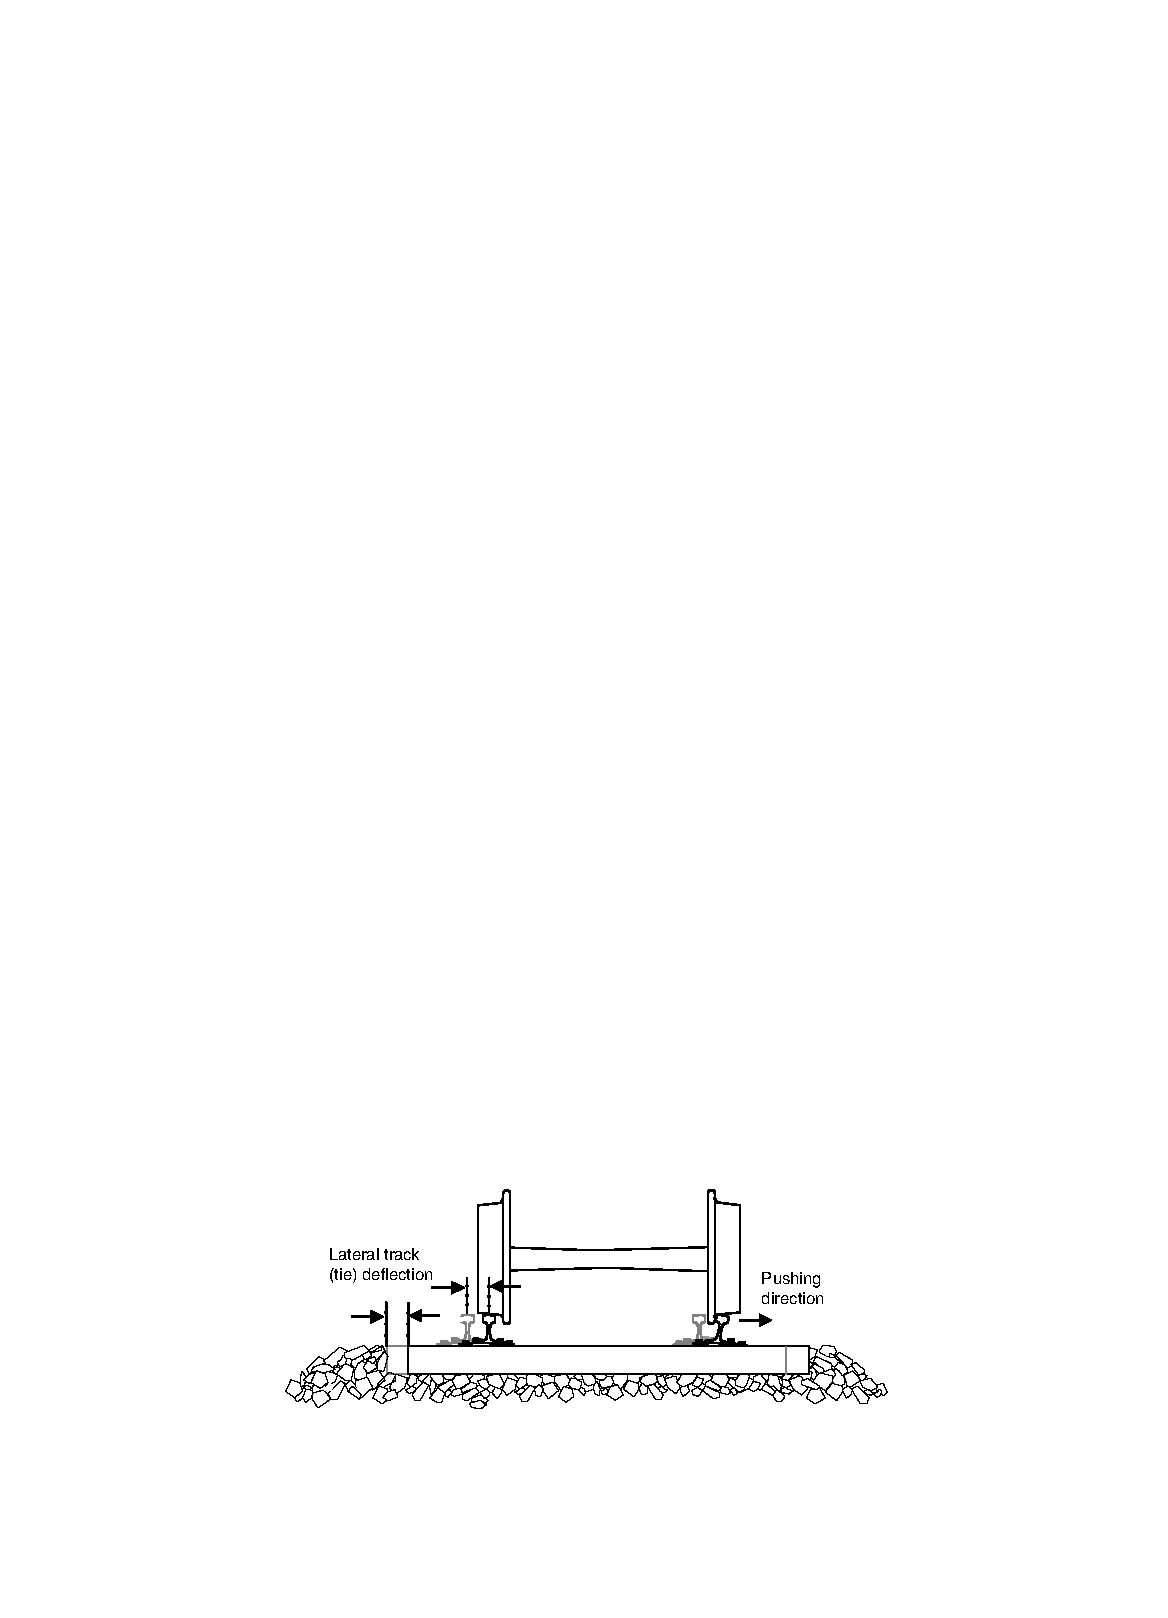
\includegraphics[width=0.8\textwidth]{lateraltrackpanelshift.pdf}
    \caption{Lateral track panel shift. Extracted from \citet[Figure8.27]{iwnicki2006handbook}}
    \label{fig:lateraltrackpanelshift}
\end{figure}

\paragraph{Panel shift criterion}
Researched by the French National Railways suggested that the limiting lateral axle load can be defined in a general expression for preventing excessive track panel shift:

\begin{equation}
    L_c = aV+b
\end{equation}

where $L_c$ is the critical lateral load and $V$ is the vertical axle load. \citet[Table 8.2]{iwnicki2006handbook} lists two groups of suggested valued of $a$ and $b$. It is possible that different values for $a$ and $b$ can be specified in different area.

\subsection{Derailment caused by vehicle lateral instability}
On tangent track, the wheelset generally oscillates around the track centre due to any vehicle and track irregularities, as shown in Figure\ref{fig:wheelsetoscillatesaroundthetrackcentre}. This movement occurs because vehicle and track are never absolutely smooth and symmetric. This self-centring capability of a wheelset is induced by the coned shape of the wheel tread. However, as speed is increased, if the whelset conicity is high, the lateral movement of wheelset, as well as the associated bogie and car body motion, can cause oscillations with large amplitude  and a well-defined wavelength. The lateral movements are limited only by the contact of the wheel flanges with the rail. This vehicle dynamic response is also termed as vehicle hunting, and can produce high lateral forces to damage track to cause derailments.

\begin{figure}[h]
    \centering
    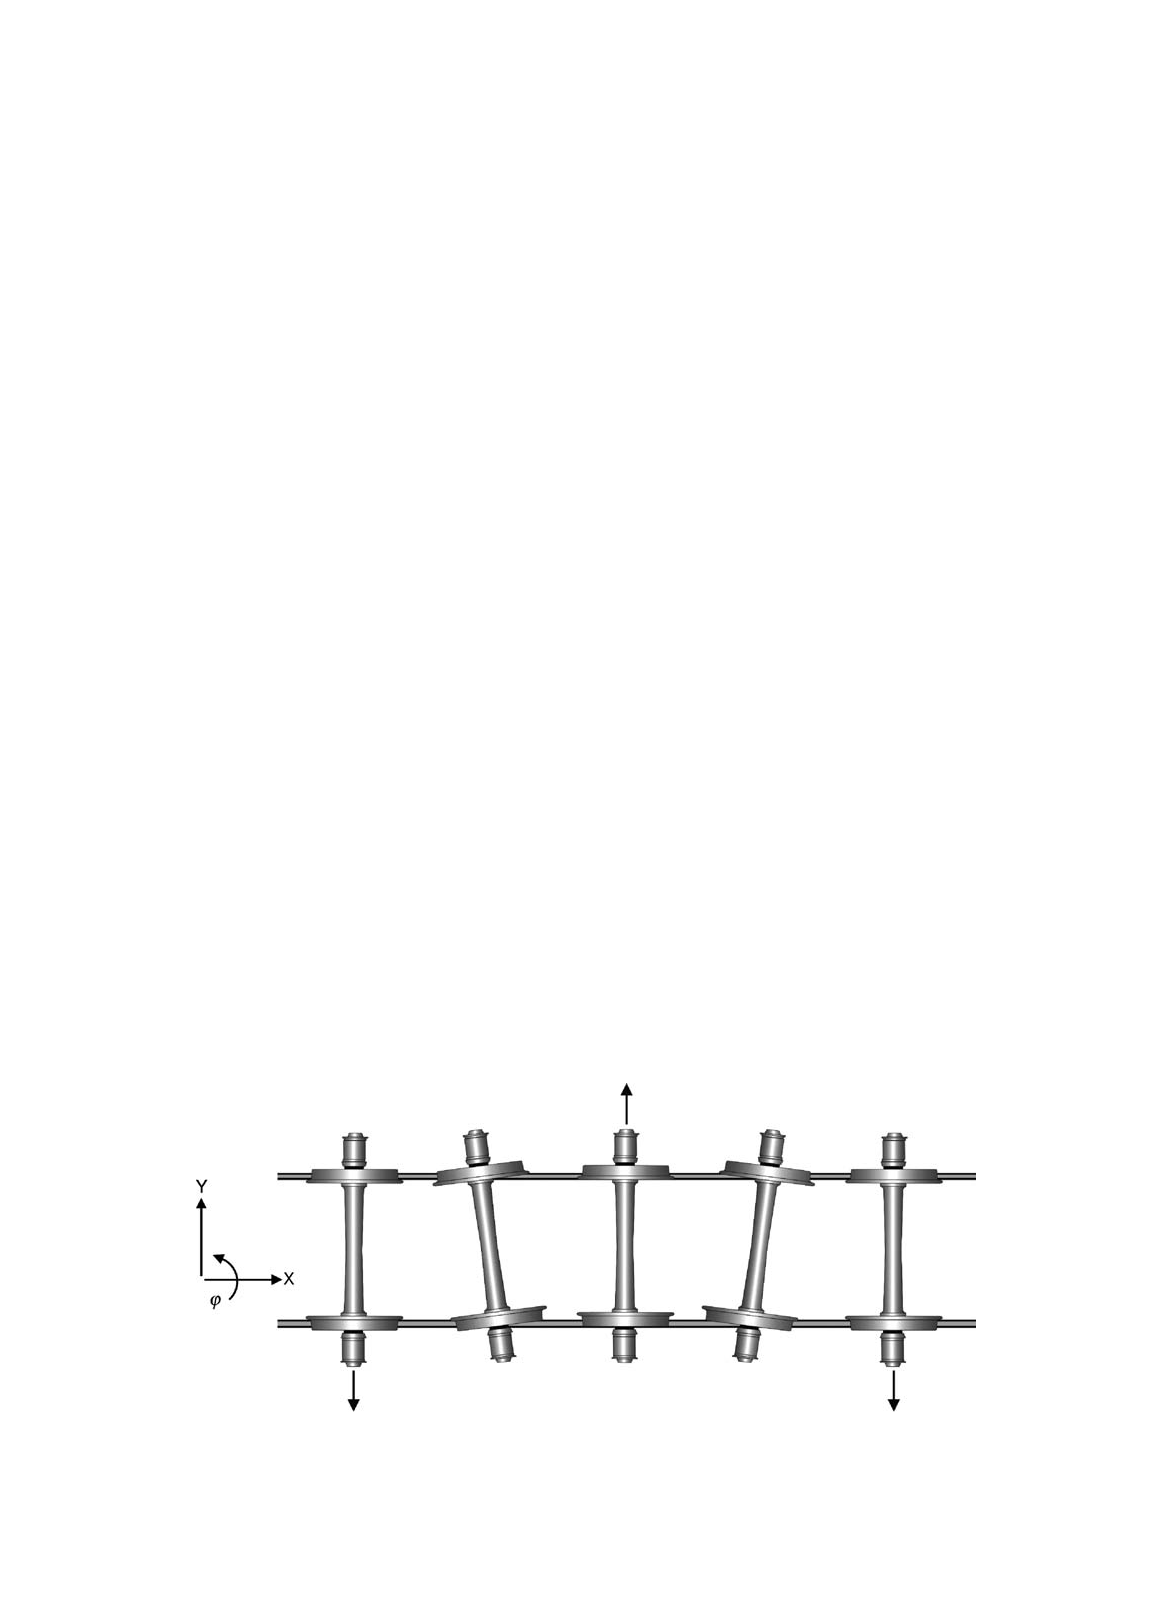
\includegraphics[width=0.8\textwidth]{wheelsetoscillatesaroundthetrackcentre.pdf}
    \caption{Wheelset oscillates around the track centre. Extracted from \citet[Figure8.28]{iwnicki2006handbook}}
    \label{fig:wheelsetoscillatesaroundthetrackcentre}
\end{figure}

Derailment cause by vehicle hunting can have derailment mechanisms of all four types discussed in the previous sections. The high lateral force induced from hunting may cause wheel flange climbing on the rail, gauge widening, rail roll-over, track panel shift, or combinations of these. The safety concerns for this type of derailment, usually occurring at higher speeds, make it an important area of study.

Hunting predominantly occurs in empty or lightweight vehicles. The critical hunting speed is highly dependent on the vehicle/track characteristics. Investigation of the critical speed for such a system with nonlinearities is to examine the vehicle response to a disturbance using a numerical solution of the equations of motion.

\subsection{Requirements for traffic serviceability(horizontal)}

The criteria Comfort Indexes for assessing ride comfort in railway vehicles proposed in \citet{12299}. This standard describes a methodology for assessing ride comfort as a function of longitudinal, vertical and transverse accelerations.

Comfort Index indicates the percentage of passengers experimenting discomfort in a specific situation. These indexes can be computed via empiric formula given in the standard, which depend on variables such as lateral acceleration, rate of change of acceleration and rolling velocity. All these values are filtered with a moving average filter that eliminates small wavelength components. Using this methodology for the computed worst-case situations, the comfort indexes have been found excellent, therefore no passenger should feel uncomfortable.
